% !TEX TS-program = pdflatex
% !TEX encoding = UTF-8 Unicode

% This is a simple template for a LaTeX document using the "article" class.
% See "book", "report", "letter" for other types of document.

\documentclass[11pt]{book} % use larger type; default would be 10pt

\usepackage[utf8]{inputenc} % set input encoding (not needed with XeLaTeX)

%%% Examples of Article customizations
% These packages are optional, depending whether you want the features they provide.
% See the LaTeX Companion or other references for full information.

%%% PAGE DIMENSIONS
%\usepackage{geometry} % to change the page dimensions
\usepackage[top=30truemm,bottom=25truemm,left=20truemm,right=20truemm]{geometry}
\geometry{a4paper} % or letterpaper (US) or a5paper or....
% \geometry{margins=2in} % for example, change the margins to 2 inches all round
% \geometry{landscape} % set up the page for landscape
%   read geometry.pdf for detailed page layout information

\usepackage[dvips]{graphicx} % support the \includegraphics command and options
\usepackage[dvips]{color}

% \usepackage[parfill]{parskip} % Activate to begin paragraphs with an empty line rather than an indent

%%% PACKAGES
\usepackage{booktabs} % for much better looking tables
\usepackage{array} % for better arrays (eg matrices) in maths
\usepackage{paralist} % very flexible & customisable lists (eg. enumerate/itemize, etc.)
\usepackage{verbatim} % adds environment for commenting out blocks of text & for better verbatim
\usepackage{subfig} % make it possible to include more than one captioned figure/table in a single float
% These packages are all incorporated in the memoir class to one degree or another...
\usepackage{amsmath,amssymb}
\usepackage{framed}
\usepackage{braket}
\usepackage[stable]{footmisc}

%%% HEADERS & FOOTERS
\usepackage{fancyhdr} % This should be set AFTER setting up the page geometry
\pagestyle{fancy} % options: empty , plain , fancy
\renewcommand{\headrulewidth}{1pt} % customise the layout...
\rhead[]{\rightmark}
\lhead[\leftmark]{}
\lfoot{}\cfoot{\thepage}\rfoot{}
\renewcommand{\chaptermark}[1]{\markboth{Chapter\ \thechapter\ #1}{}}
\renewcommand{\sectionmark}[1]{\markright{Section\ \thesection\ #1}{}}

%%% SECTION TITLE APPEARANCE
\usepackage{sectsty}
\allsectionsfont{\sffamily\mdseries\upshape} % (See the fntguide.pdf for font help)
% (This matches ConTeXt defaults)

%%% ToC (table of contents) APPEARANCE
\usepackage[nottoc,notlof,notlot]{tocbibind} % Put the bibliography in the ToC
\usepackage[titles,subfigure]{tocloft} % Alter the style of the Table of Contents
\renewcommand{\cftsecfont}{\rmfamily\mdseries\upshape}
\renewcommand{\cftsecpagefont}{\rmfamily\mdseries\upshape} % No bold!

%%% END Article customizations

%%% The "real" document content comes below...

\begin{document}
\begin{titlepage}
\begin{center}
\vspace*{100truept}
{\huge Requantization of time-dependent mean field}\\
\vspace{5truept}
{\huge for pairing collective motion in superfluid nuclei}\\
\vspace*{120truept}
{\LARGE Fang Ni}\\
\vspace*{280truept}
{\LARGE February 2019}\\ 
\end{center}
\end{titlepage} 
\newpage

\thispagestyle{empty}
\newpage

\begin{titlepage}
\begin{center}
\vspace*{100truept}
{\huge Requantization of time-dependent mean field}\\
\vspace{5truept}
{\huge for pairing collective motion in superfluid nuclei}\\
\vspace*{120truept}
{\LARGE Fang Ni}\\
\vspace{5truept}
{\LARGE Doctral Program in Physics}\\
\vspace*{200truept}
{\LARGE Submitted to the Graduate School of}\\
\vspace{5truept}
{\LARGE Pure and Applied Sciences}\\
\vspace{5truept}
{\LARGE in Partial Fulfillment of the Requirements} \\
\vspace{5truept}
{\LARGE for the Degree of Doctor of Philosophy in}\\
\vspace{5truept}
{\LARGE Science}\\
\vspace*{15truept}
{\LARGE at the}\\
\vspace{5truept}
{\LARGE University of Tsukuba}\\ 
\end{center}
\end{titlepage} 
\thispagestyle{empty}

\chapter*{Abstract}
\thispagestyle{empty}

The low-lying excited $0^+$ states in most of nuclei had been traditionally considered as either $\beta$ vibration or two-phonon excitation associated with quadrupole vibrations. However, plenty of recent experimental data indicate that not only quadrupole correlations but also pairing correlations play important roles in such excited $0^+$ states. 
%From theoretical viewpoint, 
%excited $0^+$ states in superfluid nuclei correspond to not only quadrupole vibrational mode, the elementary mode of excitation of quadrupole collective motions, but also pairing vibrational mode, the elementary mode of excitation of pairing collective motions. 
The competition between quadrupole correlations and pairing correlations causes complex and mysterious structure for the low-lying excited $0^+$ states. 
We aim to understand such excited $0^+$ states based on the time-dependent mean-field (TDMF) theory. Because quantum fluctuation is large in low-lying excitation region, we need to treat the collective motion in large-amplitude regime. However, the theoretical framework to describe pairing collective motions in the large-amplitude regime is not yet established. The nature of low-lying pairing collective motions is still unclear.

We aim at developing a new theoretical framework to describe large-amplitude collective motions associated with nuclear pairing. In our approach, the low-lying excited states are obtained in two steps: (1) solve TDMF equation to obtain the classical trajectories; (2) quantize such classical trajectories to obtain the excited states. The step 2 is called ``requantization''. 
First, we consider the pairing collective motions in multi-level pairing model. The pairing models can be classified into two classes, integrable and non-integrable systems. The former one corresponds to the two-level system and the later one corresponds to the system with three levels or more. 

In the integrable system, the requantization of TDMF is particularly feasible because we can easily find the periodic orbits. We apply three different requantization methods, canonical quantization, Fourier decomposition of the time-dependent observables, and stationary phase approximation (SPA) to the path integral. Comparing each requantization method with the exact solution, respectively, SPA turns out to be the most accurate among the three and can describe the excited states quantitatively, including two-particle transition strength. Because the requantized wave functions from SPA are given in terms of the microscopic degrees of freedom, the transition matrix elements can be calculated directly.

Unfortunately, the application of the SPA to the non-integrable system is not straightforward because finding the periodic orbits is an extremely difficult task. We propose a new theoretical approach which makes the SPA to be applicable to non-integrable systems, that is, combining the SPA with the adiabatic self-consistent collective coordinate (ASCC) method (ASCC+SPA). The concept is that we employ the ASCC to extract an integrable subspace from original TDMF phase space, and apply the SPA to the integrable subspace. 
%The detailed derivation is shown in the text.
We apply the ASCC+SPA to the low-lying excited $0^+$ states in three-level system and Pb isotopes system. We find that the ASCC+SPA can properly describe the pairing collective motions. 

We also examine the validity of the pairing collective model which assumes the pairing gap parameter and gauge angle as the phenomenological collective coordinates. We check the one-to-one correspondence between the collective coordinates self-consistently determined with the ASCC and those assumed in the collective model. We find the collective coordinate describing pairing vibration has no one-to-one correspondence between the two, in both integrable and non-integrable systems. The applicability of the collective model is limited for the nuclear pairing.

%We summarize the achievements in this thesis. We find a reasonable requantization method, SPA, from the study in integrable system. Using SPA, we construct a theoretical framework of ASCC+SPA to requantize the pairing collective motions in non-integrable system. Also, we demonstrate that it is necessary to describe the pairing vibration in the collective coordinate extracted from TDMF degrees of freedom itself, instead of the phenomenological collective coordinate, pairing gap parameter. 
With the development of computational power and numerical techniques,
the ASCC+SPA is a promising tool to elucidate the structure of mysterious low-lying excited $0^+$ states in nuclei, in near future.

\thispagestyle{empty}

\pagenumbering{roman}
\setcounter{page}{-1}
\tableofcontents
%\thispagestyle{empty}

\chapter{Introduction}
\pagenumbering{arabic}

\section{Pairing correlation in theoretical and experimental aspects}

\subsection{Superfluid nuclei}

Mean-field model is a standard tool to describe the structure of atomic nuclei. The idea of mean-field model is based on the primary theoretical framework of shell model introduced by Mayer and Jensen in 1949. Mean field picture indicates that the nucleus can be described in single-particle motion in the mean field potential created by the whole nucleons in the nucleus. Although the many-body correlations between the nucleons is extremely complicate, the single-particle motion picture can well reproduce the basic properties (e.g. radius, binding energy, separation energy, magic number) in most of nuclide. %%The most popular mean field potential is Woods-Saxon potential with spin-orbit coupling. Because 

\begin{figure}[tb]
 \begin{center}
    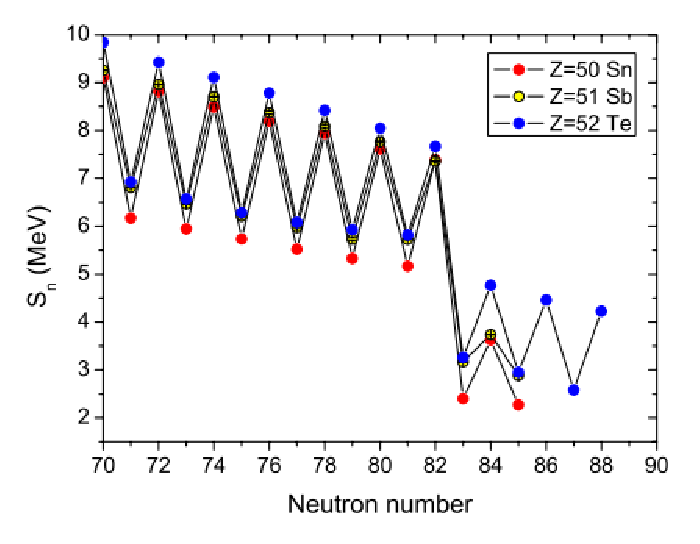
\includegraphics[width=100mm]{images/S_n.eps}
 \end{center}
  \caption{Separation energy for Sn, Sb, Te isotopes as a function of neutron number obtained from experimental data \cite{KJJ12}.}
  \label{S_n}
\end{figure}

Of course, single-particle motion picture cannot describe the nuclear system perfectly. To describe the nuclear structure more precisely, residual interactions need to be taken account. In 1950s, nuclear physicists found one of the most important residual interactions, pairing correlation. One of the clear evidences for pairing correlation detected from experiment is the separation energy difference between odd nuclei and even nuclei. Fig. \ref{S_n} shows the separation energies for Sn, Sb, and Te isotopes as a function of neutron number. The isotopes in even number of neutron have about $2\sim3$ MeV larger separation energies than the isotopes in odd number of neutron.
It is odd-even staggering (OES) effect, which is detected in whole mass region of nuclei (Fig. \ref{gap}). In this figure, $2\Delta$ corresponds to the separation energy difference between even-even nuclei and odd mass number nuclei. The approximate value is $2\Delta \approx 24A^{-1/2}$ MeV. It indicates a two-body attractive interaction should be included based on single-particle motion picture. In addition, if we examine the spin-parity of the ground states, we can find all of the even-even nuclei are $J^{\pi}=0^+$ states and most of the odd mass number nuclei have the same spin-parity as their single-particle orbit which the last nucleon fulfills in.
To explain these phenomena, it is natural to consider that the ground state of even-even nuclei consist of coupled $J^{\pi}=0^+$ pairs and the ground state of odd mass number nuclei consist of coupled $J^{\pi}=0^+$ pairs except one unpaired nucleon in last single-particle orbit. The two-body attractive interaction which couples two identical nucleons into $J^{\pi}=0^+$ state is called pairing correlation.

\begin{figure}[tb]
 \begin{center}
    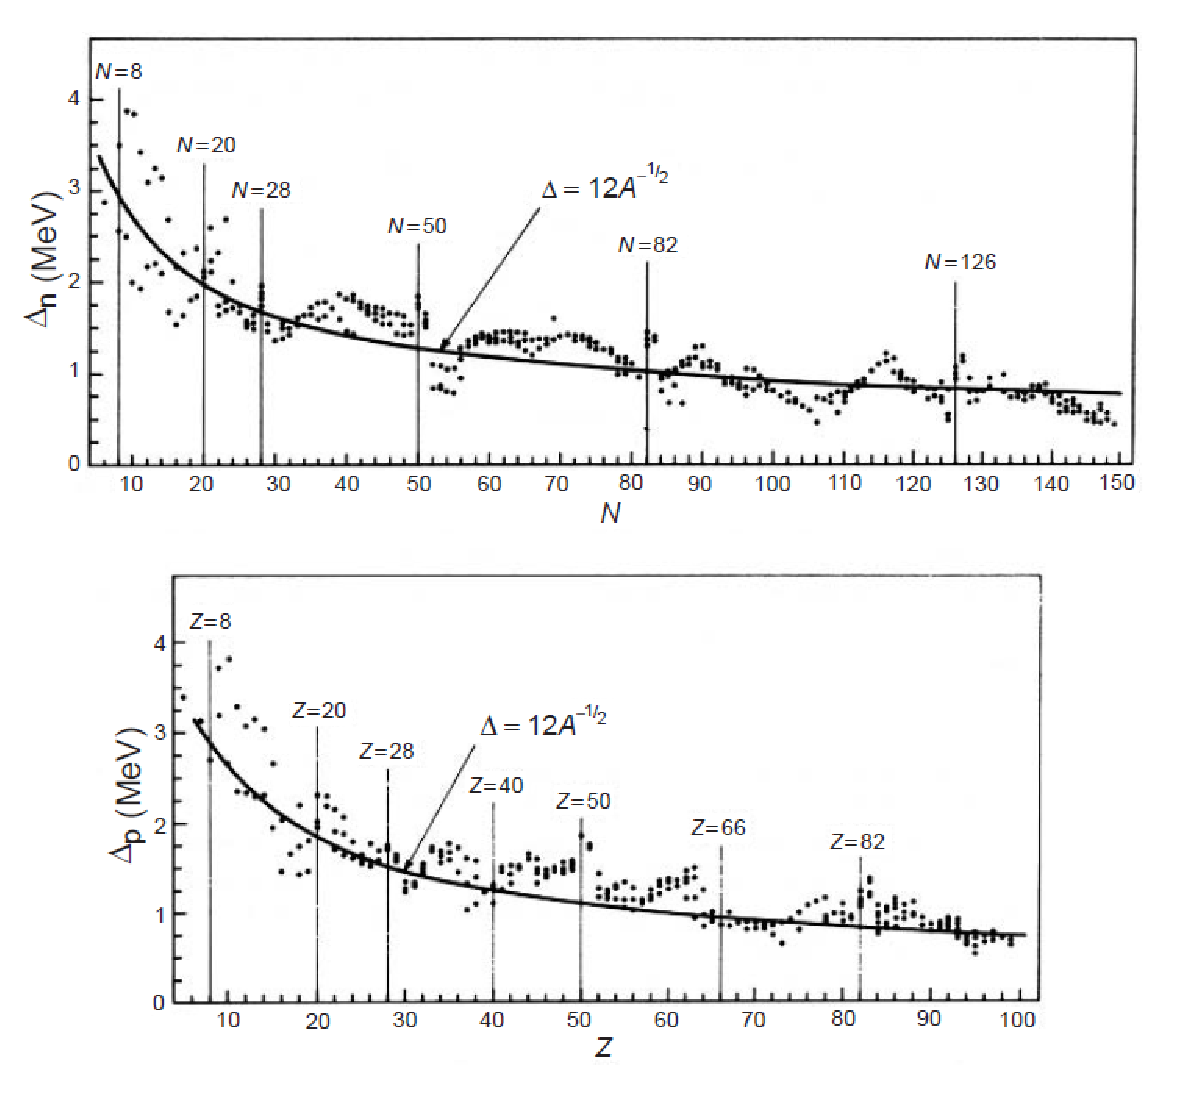
\includegraphics[width=120mm]{images/gap.eps}
 \end{center}
  \caption{The odd-even mass differences $\Delta_n$, $\Delta_p$ for neutrons and protons (Zeldes {\it et al.} {\it Mat. Fys. Skr. Dan. Vid. Selsk.}, 3, no. 5 (1967)).}
  \label{gap}
\end{figure}

Because pairing correlation is two-body interaction, a theoretical framework beyond the mean-field model seems to be necessary. However, there is a tricky approximated theory, BCS theory, enable us to describe pairing correlation within mean-field model. In BCS theory, the states with different particle number are superposed to describe the ground state. It indicates that the ground state breaks symmetry in a space, namely U(1) gauge space. With symmetry breaking, the corresponding order parameter, pairing gap $\Delta$, has finite value. Based on BCS theory, because the energy of each particle in a $J^{\pi}=0^+$ pair is $E_k=\sqrt{(\epsilon_k-\lambda)^2+\Delta^2}$, where $\epsilon_k$ is single particle energy, $\lambda$ is Fermi energy, the lowest single-particle excited state corresponds to one-pair broken state with minimum excitation energy $2\Delta$. In fact, pairing gap corresponds to the separation energy difference between even-even nuclei and odd mass number nuclei. As same as superconductivity in condensed matter physics, the superfluid nucleus is defined when $\Delta\neq0$ in ground state. Thus, BCS theory can explain the OES effect caused from pairing correlation.

After BCS theory was firstly introduced by J. Bardeen, L. Cooper, and J. R. Schrieffer in 1957, it was immediately generalized to Hartree-Fock-Bogoliubov (HFB) theory. HFB theory is the naturally extension of Hartree-Fock (HF) theory by introducing Bogoliubov transformation. Under Bogoliubov transformation, the particles become to quasiparticles, and the mean-field is extended to generalized form including pairing field. After HFB theory had been applied to nuclear physics in 1958, the structure of ground states in nuclei was examined by plenty of studies. Up to now, HFB theory is the standard mean-field theory to describe nuclear structure including pairing correlation.

% Recently, nuclear density functional theory has been developed based on HFB theory. and the computational codes are well developed. The properties of ground states in even-even nuclei are well studied by HFB theory.

%BCS theory is firstly introduced by J. Bardeen, L. Cooper, and J. R. Schrieffer in 1957 \cite{} to describe . BCS theory can describe the superconducting state or superfluid state caused by cooper pairs. In nuclear physics, the  created by pairing correlation correspond to the cooper pairs. 

%  It indicates that the ground states consist of the $J^{\pi}=0^+$ pairs is more stable than other configurations. In addition, the ground states between even-even nuclei and neighborhood odd nuclei has large gaps of binding energy. In odd nuclei, the unpaired last neutron is the last single-particle level. The odd-even mass difference  To break the $J^{\pi}=0^+$ pair, we need large energy which

%Pairing correlation plays an important role near the Fermi energy.
%\begin{figure}[htbp]
% \begin{center}
%    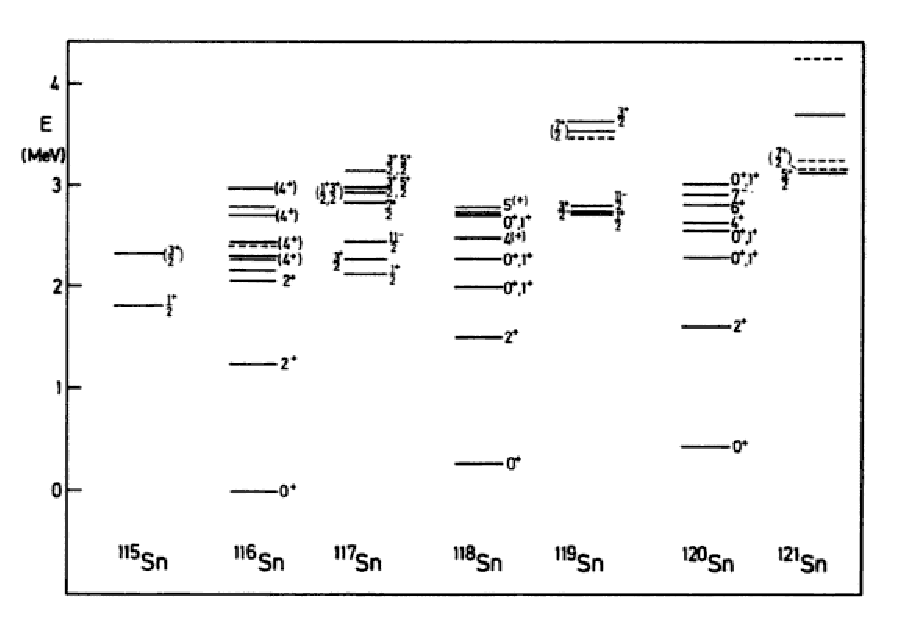
\includegraphics[width=100mm]{images/Sn_isotope.eps}
% \end{center}
%  \caption{Low-lying excited states in Sn isotopes \cite{}. The absolute values of binding energy are adjusted at 0 MeV in the ground state of ${}^{116}$Sn.}
%  \label{Sn_isotope}
%\end{figure}


\subsection{Pairing collective motion}
\label{1-1-2}

\begin{figure}[bt]
 \begin{center}
    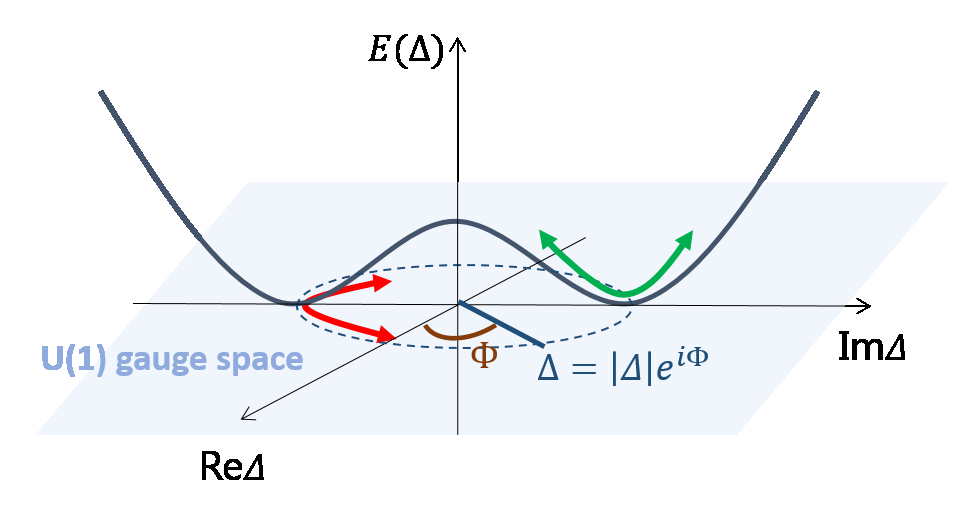
\includegraphics[width=100mm]{images/pair_coll.eps}
 \end{center}
  \caption{Schematic picture of pairing collective motion with superfluid ground state. Red  bi-direction arrow indicates pairing rotation, which rotates in $\Phi$ direction along the energy minimum circle degenerating at an absolute value of pairing gap $|\Delta|\neq 0$, in U(1) gauge space. Green bi-direction arrow indicates pairing vibration, which vibrates in $|\Delta|$ direction around one of the degenerated energy minimum points.}
  \label{Pair_coll}
\end{figure}

\begin{figure}[tb]
 \begin{center}
    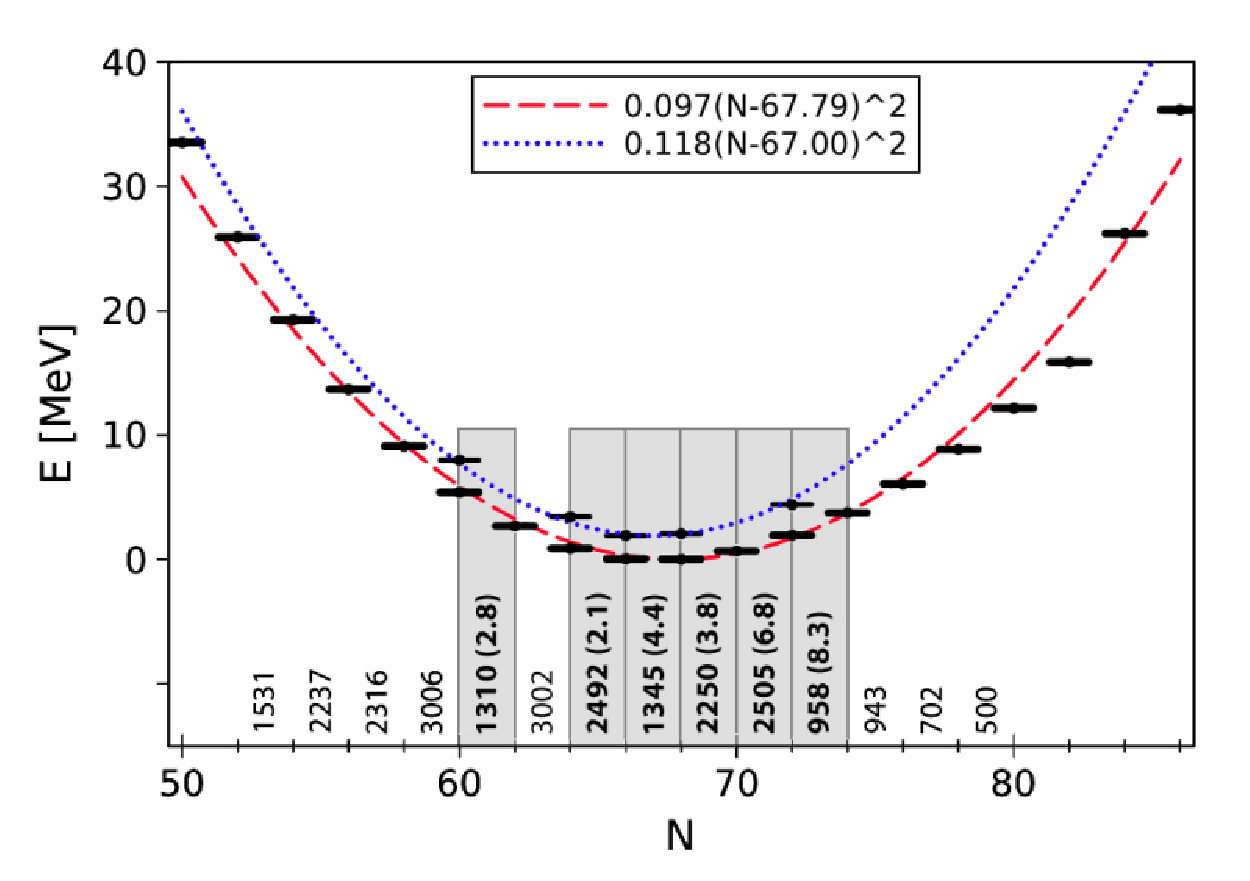
\includegraphics[width=100mm]{images/pair_rot.eps}
 \end{center}
  \caption{Experimental energies of the $J^{\pi}=0^+$ states of the Sn isotopes (ground state and pairing vibration),
populated in $(p, t)$ reactions. The heavy drawn horizontal lines
represent the values of the expression $E=-B({}_{50}^{A}{\rm Sn}_{N})+E_{exc}+
8.124A+46.33$ MeV, where $B({}_{50}^{A}{\rm Sn}_{N})$ is the binding energy
of the Sn isotopes of mass number $A$, and $E_{exc}$ is the
weighted [with $\sigma(0_i^+)$] average energy of the excited $0^+$ states
below 3 MeV. The dashed and dotted lines represent the parabolas
given in the insets, corresponding to the ground state and to
the (average) excited state-based pairing rotational bands. The
absolute values of the $g.s.\to g.s.$ integrated cross sections (in $\mu$b units) are given (perpendicular) to the abscissa, as a function
of $N$. The values in the shaded areas correspond to the experimental values, while the remaining values correspond to theoretical
predictions. For the first group (experimental), the relative
(in \%)$(p, t)$, pairing vibrational, cross sections $\sum_i\sigma(g.s.\to 0_i^+)$
normalized with respect to the ground state cross sections are in parenthesis. The detailed information are written in \cite{PF11}.}
  \label{pair_rot}
\end{figure}


Due to the superfluid state breaks the symmetry in U(1) gauge space, there are two types of elementary modes of excitation for pairing collective motion in nuclei. The elementary modes of excitation are Nambu-Goldstone (NG) mode, pairing rotational mode, recovering the broken symmetry in U(1) gauge space, and Higgs mode, pairing vibrational mode, fluctuating around the energy minimum point.

First, we discuss the pairing rotation. In classical picture, pairing rotation is the motion which the system rotates in the U(1) gauge space (red bi-direction arrow in Fig. \ref{pair_rot}). The motion is described by the coordinate, gauge angle $\Phi$, and the corresponding momentum, total particle number $N$. 
%It is similar to normal rotation in 3D space which described by the angles ($\theta_x, \theta_y, \theta_z$) and their conjugate angular momenta ($J_x, J_y, J_z$). 
Of course, $N$ is a constant of motion. In quantum picture, if we assume the ground state of $N_0$ particle system as the ``ground state'', the ground states in $N=N_0\pm2, N_0\pm4,\cdots$ correspond to the ``excited states'' in the pairing rotational mode. The excitation energy is $E_{\rm rot}^{\rm pair}=\frac{(N-N_0)^2}{2\mathcal{J}}$, where $\mathcal{J}$ is the pairing-rotational moment of inertia. In experiment, the pairing rotational band is expected to be observed in even-even isotope chain or even-even isotone chain in open-shell nuclei. A clear observation is found in Sn isotopes shown in Fig. \ref{pair_rot}. Except a constant value and linear term with respect to mass number $A$, we can find the energies of ground states consist of a parabolic line - pairing rotational band. Recently, the systematic study for the pairing-rotational moment of inertia has been done in Ref. \cite{HN16}. The experimental moments of inertia obtained from two neutron(proton) separation energies have excellent correspondence with the theoretical moments of inertia obtained from NG mode in quasiparticle random phase approximation (QRPA) \cite{TV61}, not only for the spherical nuclei, but also for the deformed nuclei. Because the pairing-rotational moments of inertia are free from ambiguities caused from odd-even system, they are supposed to be excellent indicators of pairing correlation rather than pairing gaps.

Next, we discuss the pairing vibration. We emphasize that there are two types of pairing vibrations, one vibrating around a normal ground state ($\Delta\approx 0$), and the other vibrating around superfluid ground state ($\Delta\neq 0$). The properties of the two are quite different. 
%The former one is well understood because the structure of the excited $0^+$ states are $2np2nh$ configurations, detected from the energy spectra around ${}^{208}$Pb. 
Here, we only focus on the later case.
In classical picture, the system vibrates around one of the degenerated energy minimum points. Depending on the intrinsic structure, various pairing vibrations are able to exist in one nucleus. 
%In general, the motion is supposed to be described by the coordinate, pairing gap $\Delta$, and its corresponding momentum\footnote{Because $\Delta$ is order parameter, it is naturally supposed to be the coordinate to describe the pairing vibration in previous studies. However, we found $\Delta$ is not proper coordinate in most of case from our study. The detail is discussed in Chapter 3 and 4.}.
In quantum picture, if we assume the ground state of $N_0$ particle system as the ``ground state'', the excited states in $N=N_0, N_0\pm2, N_0\pm4,\cdots$ correspond to the ``excited states'' of pairing vibrational mode. The excitation energy is $E_{\rm vib}^{\rm pair}=n_{\alpha}\hbar\omega$, where $n_{\alpha}$ is the number of phonon and $\alpha$ is the label to distinguish different pairing vibrational modes. Because $2\Delta$ is the minimum energy to break one-pair, the collectivity is dominant when $E_{\rm vib}^{\rm pair}<2\Delta$. Thus, low-lying excited $0^+$ states in even-even nuclei have strong collectivity associated with pairing vibration. Except the region around the magic number, excited $0^+$ states below $2\Delta$ exist in most of even-even nuclei. However, it is difficult to observe the signatures for pairing vibration directly from experiment. The properties of pairing vibration in nuclei are not well understood up to now.
% because the multipole correlations interfere the pairing correlation significantly

The signatures for pairing collective motion can also be observed from the two-neutron(proton) transfer reaction \cite{BHR73}, such as $(p, t)$, $(t, p)$, and $({}^3{\rm He}, n)$. The cross sections of two particle transfer reaction strongly depend on the matrix elements of $J^{\pi}=0^+$ pair-transition operators (e.g. pair-additional transition: $\sigma( P_{ad};0_{\alpha}^+(N) \to 0_{\beta}^+(N+2))\sim |\braket{N+2,\beta|\sum_k a^{\dag}_k a^{\dag}_{\bar{k}}|N,\alpha}|^2$). From theoretical prediction, the pairing correlation is known to enhance $\sigma(g.s.\to g.s.)$ and decrease $\sigma(g.s.\to 0_{ex}^+)$ significantly, hence, $\sigma(g.s.\to 0_{ex}^+)/\sigma(g.s.\to g.s.)\ll 1$ is expected in superfluid system. One example of $(p, t)$ reactions is demonstrated in Fig. \ref{pair_rot}. As mentioned in previous paragraph, the ground states of even-even Sn isotopes consist of a pairing rotational band. In such situation, the intraband transition is dominant with respect to the interband transition. Therefore, the cross sections of two-neutron transfer reaction is consistent with theoretical prediction. In general, the ratio $\sigma(g.s.\to 0_{ex}^+)/\sigma(g.s.\to g.s.)$ for two-neutron(proton) transfer reaction are excellent indicators to describe the collectivity of pairing dynamics.

\subsection{Mysterious excited $0^+$ states and pairing dynamics}
In most of nuclei, the structure of excited $0^+$ states in a low-lying region (a few MeV excitation) is complicate and unclear \cite{HW11}. The reason is that not only pairing correlations but also deformations and multipole correlations influence the excited $0^+$ states significantly. The various correlations competing with each other construct plenty of mysterious excited $0^+$ states. We present several examples for these excited $0^+$ states observed from experiment.

After the concept of pairing vibration was introduced, it encountered the problem for the large asymmetry cross sections between $(p, t)$ and $(t, p)$ reaction in actinide region (e.g. Th, U, Pu, Cm) observed from experiment. In low-lying energy region, the cross section of $\sigma(g.s.\to 0_{ex}^+)$ is about $15\%$ of $\sigma(g.s.\to g.s.)$ for $(p, t)$ reaction \cite{MEFSS70, MEFSS72}, while the signal of $\sigma(g.s.\to 0_{ex}^+)$ is extremely weak for $(t, p)$ reaction \cite{Cas72}. To explain such phenomena, the coexistence of both oblate shape and prolate shape in one state, and the mixing of pairing correlations between oblate and prolate shape was suggested \cite{GJV71,RK72}. Another interpretation for such phenomena is using microscopic interaction, including multipole pairing correlations and quadrupole particle-hole interactions \cite{RB76}. Although the approaches between these studies are different, they reproduced the asymmetry cross sections of two-neutron transfer reaction in actinide region. These studies hinted the importance of the quadrupole correlations in low-lying excited $0^+$ states. 

We can consider the excited $0^+$ states from common viewpoint, liquid drop with surface vibration. Bohr collective model, which is well-known and successful model describing the quadrupole collective motions in nuclei \cite{BM75} has been constructed based on the idea of liquid drop. The $0_2^+$ states in the model correspond to $\beta$ vibration and the first $2^+$ state in $K=2$ bands correspond to $\gamma$ vibration, in quadrupole deformed nuclei. Also, their rotational bands exist in each vibrational mode. The nuclei in rare earth region (e.g. Sm, Gd, Dy, Er, Yb, Hf, W), well deformed nuclei, had been supposed to be the typical examples of quadrupole collective motions in the early days. 
With the development for extracting $B(E2)$ values from experiment, however, the doubt whether $0_2^+$ states in rare earth region is $\beta$ vibration arose in the last decades \cite{G01, Kulp08, SS11}. They found that only a part of $B(E2)$ values related to the $0_2^+$ states agree with the predicted $B(E2)$ values in pure $\beta$ vibration picture. Moreover, for $E0$ transition, very few $0_2^+$ states satisfies the range of $\rho^2(E0)$ values which the $\beta$ vibrational picture predicts. On the other hand, they detected strong cross sections $\sigma(g.s.\to 0_{2}^+)$ in both $(t, p)$ and $(p, t)$ reactions. These results suggest that $\ket{0_2^+}$ in rare earth region are not pure $\beta$ vibrational states, but some states mixing with pairing correlations.

\begin{figure}[tb]
 \begin{center}
    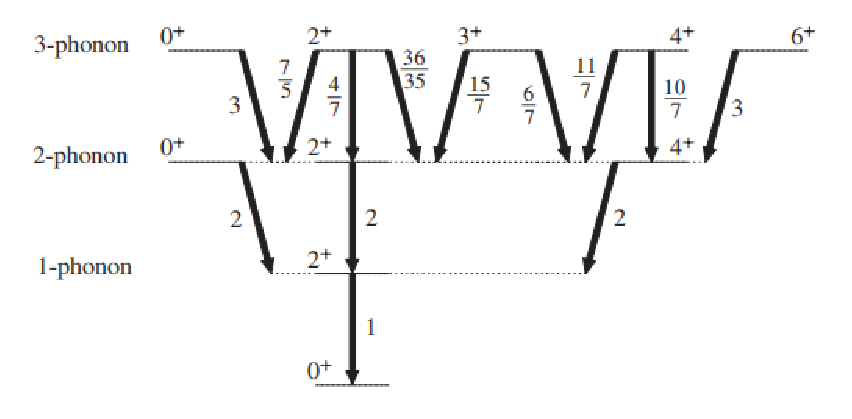
\includegraphics[width=100mm]{images/phonon.eps}
 \end{center}
 \begin{center}
    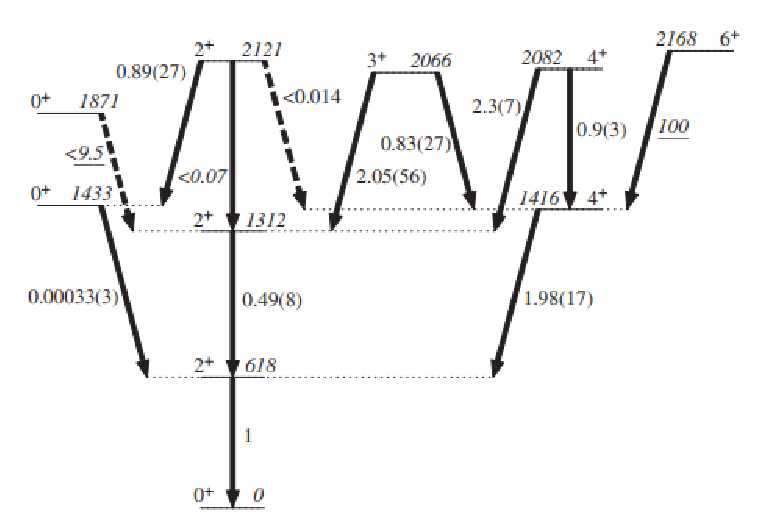
\includegraphics[width=100mm]{images/112Cd.eps}
 \end{center}
  \caption{$B(E2)$ values, relative to the $B(E2; 2_1^+\to 0_1^+)$ value, and energy spectra in phonon excitation picture. Upper panel: expected $B(E2)$ values for a quadrupole harmonic vibrator. Lower panel: data observed for ${}^{112}$Cd. Dashed transitions indicate an unobserved transition. Detailed information is discussed in Ref. \cite{GW10}.}
  \label{112Cd}
\end{figure}
The mystery of excited $0^+$ states exist not only in deformed nuclei, but also in spherical nuclei. A best example is the structure of $0_2^+$ or $0_3^+$ states in Cd isotopes observed in recent experiment \cite{GW10}. The lower part of Fig. \ref{112Cd} shows the excitation energy and $B(E2)$ transition strength in ${}^{112}$Cd. Comparing with the typical values for the ideal quadrupole harmonic vibration in spherical nuclei shown in the upper part of Fig. \ref{112Cd}, we can find that the observed excitation energy spectra have good coincidence with phonon excitation picture. The $0_2^+$ or $0_3^+$ states seem to be interpreted as two-phonon or three-phonon excitation. However, the $B(E2)$ values are quite different between the two, especially for the no observed decay from $0_{2ph}^+$ to $2_1^+$ state. Such phenomena are also seen in other Cd isotopes. The configuration of these $0^+$ states are supposed to be not pure phonon excitation, but proton pair-excitation between $2p_{1/2}$ and $1g_{9/2}$ orbits from the hint of the ground state configurations of Ag isotopes \cite{HW11}. The pairing should play an important role if the excited $0^+$ states are described by pair-excitation.

%Collective motion is the essential idea to explain the excited states in nuclei. The quadrupole collective motion described by the quadrupole deformation parameters $\alpha_{2\mu} (\mu=\pm2,\pm1,0)$ is known as the most typical collective motion. In the framework of quadrupole collective motion, the low-lying excited $0^+$ states can be roughly categorized into two types: quadrupole vibration emerging above two-phonon excitation in spherical nuclei, and $\beta$ vibration emerging in quadrupole deformed nuclei. The excitation energies and $B(E2)$ transition strength is well understood under harmonic approximation.

\section{Motivation of this study}
We aim to understand the low-lying excited $0^+$ states ($\sim$ a few MeV excitation) from nuclear many-body theory. As mentioned above, pairing correlation plays a significant role in such excited $0^+$ states. We need to understand the nature of the pairing dynamics in nuclei. We discuss the theoretical approach to describe the pairing dynamics in the following.

\subsection{Theoretical problem}

Time-dependent mean-field (TDMF) theory is a standard theory to describe the nuclear dynamics. In principle, TDMF enables us to describe the collective motions from the microscopic degrees of freedom without any artificial parameters. Inclusion of the pairing correlation leads to the time-dependent Hartree-Fock-Bogoliubov (TDHFB) theory, which has been utilized for plenty of nuclear structure and reaction studies \cite{NMMY16}.

%QRPA
Quasiparticle random phase approximation (QRPA) theory, which correspond to the small amplitude approximation of TDHFB, is known as the most common approach to describe the structure of collective excited states. From a number of studies, the giant resonances (locating at a few MeV $\sim$ dozens of MeV excitation with broad width) can be well described by the QRPA \cite{Eba10, YN11, YN13, SL13-2}. With density functional formalism, recently, QRPA equation can be solved in finite amplitude method (FAM) \cite{Na07}. FAM, which reduce the computational time significantly, enables the linear response calculation for deformed nuclei in allowable computational time. 
%and is becoming the standard way to solve the QRPA equation numerically. 
The QRPA is not only useful to predict the collective motions which have not been observed, such as those in exotic nuclei, but also can become the basic concept of a theoretical framework beyond the linear regime. On the other hand, the QRPA description for the low-lying collective excited states is not as good as the giant resonances. The effects of anharmonic vibration and shape coexistence are often important in low-energy region \cite{HW11}, while QRPA is nothing but harmonic approximation. For example, the excitation energies of $0_2^+$ states in rare-earth region have large deviation between QRPA calculations and experimental data \cite{TE11}. 

%Large amplitude motion, Adiabatic approach
To describe the low-lying excited states, especially for the excited $0^+$ states, we need to introduce the large-amplitude motions beyond the linear regime.
Collective model, which is designed by a couple of collective coordinates and their collective potential and mass parameters, is useful for describing the large-amplitude dynamics. The most popular phenomenological collective model is Bohr collective model, five-dimensional collective Hamiltonian (5DCH) with the quadrupole deformation parameters $(\beta,\gamma)$ and the Euler angles $(\phi,\theta,\psi)$. It has been applied to describe the low-lying excited states in realistic nuclei, with the construction of the collective potential and mass parameters from the microscopic degrees of freedom \cite{NMMY16}. However, the pairing degrees of freedom are not explicitly included in the Bohr collective model. As discussed in Sec. \ref{1-1-2}, the pairing vibrational degrees of freedom supposed to be a key ingredient to understand the low-lying  excited $0^+$ states. We have great interest for the collective coordinates describing the pairing corrective motions.

The discussion for the collective model describing the pairing collective motions is not so much. The first study was introduced by Bes. et al. \cite{BBPK70}. They constructed phenomenological pairing collective model by two degrees of freedom, the pair deformation parameter (pairing gap) $\Delta$ and the global gauge angle $\Phi$. After the pairing collective model was formulated, it was combined with the Bohr collective Hamiltonian and applied to describe the nuclear structure \cite{GPBW85, ZPPRS99, P07}. 
In Ref. \cite{ZPPRS99}, the excitation energy and $B(E2)$ transition are improved by introducing pairing degrees of freedom. On the other hand, the wave function of ground state from collective model looks like unusual because the gap parameter $\Delta_{vib}$ at the peak of the pairing collective wave function is smaller than the pairing gap $\Delta_{eq}$ obtained from BCS equation. 
%There is no further discussion about the unusual behaviors. Also, two-particle transition strength is hardly discussed in the collective model.
%The problem is supposed to be the phenomenological degrees of freedom for pairing collective motion. 

The question is that whether the pair deformation parameter $\Delta$ is proper to describe the pairing vibration, as the quadrupole deformation parameters $Q_{2\mu} (\mu=\pm2,\pm1,0)$ describing the quadrupole surface vibration. From the nature viewpoint, the time evolution of $Q_{2\mu}$ correspond to nuclear vibrations in liquid drop picture, while the time evolution of $\Delta$ is difficult to be imagined as a shape vibration. We need to explore more to understand the nature of pairing dynamics in large-amplitude regime. 

\subsection{Our approach}

To understand pairing dynamics in large-amplitude regime, we think that it is important to find the collective coordinates describing the pairing collective motions from the TDHFB dynamics itself without any assumption. Apart from the realistic nuclear system, as the first step, we study the pairing collective motions in pairing model, which only contains the monopole pairing correlation in two-body interaction. In this model, the collective motions obtained from TDHFB degrees of freedom are pure pairing collective motions.

In fact, the TDHFB degrees of freedom equal to the number of single-particle level, in pairing model. Furthermore, the TDHFB degrees of freedom consist of one constant of motion, pairing rotation, and other intrinsic degrees of freedom. One-level system, which contains only one pairing rotational mode, is well understood (seniority scheme in the textbook \cite{RS80}). All we have to do is to study the multi-level system. We divide the multi-level system into two classes, two-level system and the system more than three-level. The former one is two-dimensional integrable system. We have two explicit coordinates to describe pairing rotation and pairing vibration, respectively. The later one is non-integrable system. The collective coordinate describing the pairing vibrational mode is not explicit. However, adiabatic self-consistent collective coordinate (ASCC) method  enables us to find such collective coordinate decoupled from other intrinsic degrees of freedom, without any artificial assumption \cite{MNM00, N2012}. 

With the obtained collective coordinates, we quantize them to derive the collective excited states. We call this procedure as ``requantization''. The typical requantization method is Pauli's prescription, a type of canonical quantization, which has been applied to requantize the collective Hamiltonian, such as 5DCH \cite{KB67} and pairing collective Hamiltonian \cite{BBPK70}. However, there is no guarantee whether Pauli's prescription is proper. In addition, Pauli's prescription is not available for the general collective Hamiltonian including the higher-oder terms of momenta. Moreover, canonical quantization is not the only approach for requantization. Actually, the requantized results depend on the requantization methods significantly, especially for the pairing collective motions.
%The requantization problem is serious to describe the pairing collective motions. 
%To explore a proper requantization procedure, we introduce other possible requantization methods. The surprising point is that the value of two-particle transition strength, a indicator of pairing collective motions, depends on the requantization method significantly 
After trial and error, eventually, we find that the requantization approach following the path integral form is most proper. A stationary-phase approximation (SPA) to the path integral, one of the requantization methods, can describe the pairing collective motions quantitatively. The detailed information is shown in Chap. \ref{integrable}.
On the other hand, SPA itself is available only for the integrable system. In order to apply SPA to the general non-integrable system, we construct a new requantization theoretical framework, ASCC+SPA. This requantization method can describe the pairing dynamics properly. Moreover, the ASCC+SPA is available not only for pairing collective motions, but also for any types of collective motions. In this thesis, the keyword ``SPA'' emerges frequently.

%Based on this method, we also constructed the theoretical framework for the general TDHFB dynamics.

%Because pairing model is exact solvable model, we can the collective excited states from requantization compare with the exact solution. 
%We hope that we can understand the pairing collective motion 

\section{Outline of this thesis}
This thesis is organized as follows. Chap. \ref{chap2} is the preparation for the main discussion of the thesis. We show the pairing model in this chapter. Because pairing model is exact solvable model, we give the recipe for the exact solution in the former part. In the later part, we derive the TDHFB equation for the pairing Hamiltonian in explicit form. 
%The constant of motion, pairing rotation, is also 

The main achievements of our study are shown in Chap. \ref{integrable} and Chap. \ref{non-integrable}. Chap. \ref{integrable} discuss the pairing collective motions in integrable system (two-level system). We applied three different requantization methods, canonical quantization, Fourier decomposition, and SPA to describe the pairing collective motions. The obtained excitation energies and wave functions from each method are compared with exact solution. Chap. \ref{non-integrable} refers the pairing collective motions in non-integrable system. According to the achievement in Chap. \ref{integrable}, we propose a new requantization method, ASCC+SPA. We explain the theoretical framework of ASCC+SPA in the former part, and discuss the result for pairing collective motions from ASCC+SPA in the later part.

Also, we discuss the validity of the collective model treatment in Chap. \ref{collective}. We analyze the one-to-one correspondence between the pairing gap parameter and the collective coordinate obtained from TDHFB dynamics itself in both integrable system and non-integrable system. 

In Chap. \ref{conclusion}, we summarize our achievements from the study. Moreover, we discuss the remaining problems and perspective of ASCC+SPA, toward the realistic nuclear system.

%The detailed derivations 




\clearpage{\pagestyle{empty}\cleardoublepage}
\chapter{Pairing model}
\label{chap2}

We introduce the pairing model in this chapter. The Hamiltonian of pairing model is
\begin{align}
	H &= \sum_{\alpha=1}^L \epsilon_{\alpha} n_{\alpha} - g \sum_{\alpha\beta} S_{\alpha}^+ S_{\beta}^- ,
\end{align}
where
\begin{align}
	n_{\alpha} &= \sum_m a^{\dag}_{j_\alpha m}a_{j_\alpha m} \\
        S_{\alpha}^{+} &= \sum_{m>0}a_{j_\alpha m}^{\dag}a_{j_\alpha \overline{m}}^{\dag} ,
\quad   S_{\alpha}^{-} = S_{\alpha}^{+\dag} .
\label{S_+}
\end{align}
In $L$ single-particle level system, each single-particle energy $\epsilon_{\alpha}$ possesses $(2\Omega_{\alpha})$-fold
degeneracy ($\Omega_{\alpha}=j_{\alpha}+1/2$)
and $\sum_{m>0}$ indicates the summation over $m=1/2,3/2,\cdots,$ and $\Omega_{\alpha}-1/2$. $\overline{m}$ indicates the time reversal quantum number with respect to $m$. The strength of pairing correlation is represented by coupling constant $g$. We also define a seniority $\nu_{\alpha}$, which is the number of unpaired particles in each level. The total number of unpaired particles is $\nu=\sum_{\alpha}\nu_{\alpha}$. The unpaired particles have no pairing interaction, and play a part in Pauli blocking effect.\par
In one-level system ($L=1$), the pairing dynamics is well understood. The analytic solution of the total energy is
\begin{align}
	E_{\nu}(N) = \epsilon N - \frac{1}{4}g(N-\nu)(2\Omega-N-\nu+2) .
	\label{onelevel}
\end{align}
The pairing rotational band created by the pairing correlation is completely parabolic with the pairing-rotational moment of inertia $2/g$. Also, the excited states in a specified $N$ is only described by the quantum number $\nu$. For example, the first excited state in even particle system is $\nu=2$ state, which correspond to one $J^{\pi}=0^+$ pair broken state.\par
The non-explicit dynamics arises in multi-level pairing model ($L\ge 2$). The pairing rotational mode includes higher order terms of $N$ due to the shell effect. In addition, several pairing vibrational modes emerge. The pairing vibration is not single particle motion specified by $\nu_{\alpha}$, but a collective motion arisen from $J^{\pi}=0^+$ pairs. In order to solve the multi-level pairing Hamiltonian, we explain the numerical exact solution. Also, we derive the TDHFB equation to study the mean-field picture of pairing collective motions.

\section{Exact solution}
The eigenvalues and eigenvectors can be solved exactly in pairing model. There are two major methods to obtain the exact solutions, diagonalization in quasispin space and Richardson equation.

\subsection{Diagonalization in quasispin space}
We introduce SU(2) quasispin operators fulfilling the follows commutation relation
\begin{equation}
  [S_{\alpha}^0,S_{\beta}^{+}] = \delta_{\alpha\beta}S_{\alpha}^{+},\hspace{20pt}[S_{\alpha}^{+},S_{\beta}^{-}] = 2\delta_{\alpha\beta}S_{\alpha}^{0}. 
  \label{SU2commu}
\end{equation}
If we set 
\begin{align}
  S_{\alpha}^0 &= \frac{1}{2}(\sum_ma_{j_\alpha m}^{\dag}a_{j_\alpha m}-\Omega_{\alpha})
  \label{S_0}
\end{align}
and $S_{\alpha}^+, S_{\alpha}^-$ as in (\ref{S_+}), the commutation relation (\ref{SU2commu}) is fulfilled. Using quasispin operators, the Hamiltonian can be represented by quasispin operators
\begin{align}
	H &= \sum_{\alpha} \epsilon_{\alpha} (2S_{\alpha}^0+\Omega_{\alpha}) - g \sum_{\alpha\beta} S_{\alpha}^+ S_{\beta}^- .
\end{align}
Therefore, any states $\ket{\psi}$ belong to SU(2)$\otimes\cdots\otimes$SU(2) Hilbert space, and can be expanded in the basis $\ket{S_1,S_1^0;\cdots;S_{\alpha},S_{\alpha}^0;\cdots}$
\begin{equation}
  \ket{\psi} = \sum_{S_1^0,\cdots\,S_{\alpha}^0,\cdots}c_{S_1^0,\cdots\,S_{\alpha}^0,\cdots}\ket{S_1,S_1^0;\cdots;S_{\alpha},S_{\alpha}^0;\cdots} .
\end{equation}

We consider the physical meaning of the quasispin space. Because $S_{\alpha}^+$ and $S_{\alpha}^-$ correspond to the creation and annihilation operators with respect to the $J^{\pi}=0^+$ pairs in each level, the quasispin space is decoupled from the space which the unpaired particles belong to. 
Also, $S_{\alpha}^0$ is related to the occupation number in each level. $S_{\alpha}^0=-S_{\alpha}$ is the minimum value corresponding no $J^{\pi}=0^+$ pair in the level and $S_{\alpha}^0=S_{\alpha}$ is the maximum value corresponding full of $J^{\pi}=0^+$ pairs in the level. Because $\nu_{\alpha}$ plays a part in Pauli blocking effect in the level, the absolute value of quasispin $S_{\alpha}$ is
\begin{equation}
  S_{\alpha} = \frac{1}{2}(\Omega_{\alpha}-\nu_{\alpha}).
\end{equation}

The dimension of the model space is $D=\prod_{\alpha}(2S_{\alpha}+1)$. However, $[H,N]=0$ indicates that the Hamiltonian is block diagonal with respect to the total particle number $N$. The model space can be reduced after we extract the combination of $\{S_{\alpha}^0\}$ fulfilling
\begin{equation}
  N = \sum_{\alpha} (2S_{\alpha}^0+2S_{\alpha}+\nu_{\alpha}) .
\end{equation} 
For example, we consider the dimension of the single particle levels between the magic number 50 and 82. Under spherical symmetry, we have five single particle levels, $d_{5/2}$, $g_{7/2}$, $s_{1/2}$, $d_{3/2}$, and $h_{11/2}$. The corresponding degeneracy is $\{\Omega_{\alpha}\}=\{3,4,1,2,6\}$. If we only consider the case for$\nu_{\alpha}=0$, the dimension for the system is $D=840$. On the other hand, under a specified $N$, the dimensions are 105 for $N=14$ and 91 for $N=20$.

\subsection{Richardson equation}
As mentioned above, diagonalizing the Hamiltonian is simple method to obtain the exact solution.
However, diagonalization is time consuming when the model space becomes large. The calculation time is proportional to the cubes of the dimension of the model space. For example, there are 16 single particle levels between the magic number 50 and 82 in deformed nuclei. Because the dimension for the system is $D=2^{16}=65536$, the calculation time in deformed system is $\sim 10^5$ times as much as the case in spherical system. \par
The alternative method to obtain the exact solution is to solve Richardson equation. The idea was introduced by R. W. Richardson \cite{Richardson1, Richardson2, Richardson3, Richardson4, Richardson5}. We divide the total energy into two parts
\begin{align}
  E &= \braket{\psi|H|\psi} \\
  &= \sum_{\alpha} \epsilon_{\alpha} \nu_{\alpha} + \sum_{m=1}^M E_{m} .
\end{align}
The first term is the energy of unpaired particle, and the second term is the total energy of $J^{\pi}=0^+$ pairs. The pair-energy $E_{\alpha}$ is derived from the non-linear equations
\begin{equation}
  1 - g\sum_{\alpha} \frac{\Omega_{\alpha}-\nu_{\alpha}}{2\epsilon_{\alpha}-E_{\alpha}} + 2g\sum_{n(\neq m)}^M \frac{1}{E_{n}-E_{m}} = 0 .
\end{equation}
$M$ indicates the number of $J^{\pi}=0^+$ pairs in the system, and equals to the numbers of the non-linear equations. $E_{m}$ can become not only real numbers, but also complex conjugate pairs when $M\ge 2$. 

We solved the non-linear equations numerically in general. If we input a set of initial values $E_{m}^{0}$ into the equations, the values will converge by using proper numerical algorithm such as Newton-Raphson method. The difficult point is that we cannot directly specify the number of excitation from the obtained excitation energy because the converged excitation energy $\sum_{m=1}^M E_{m}$ can be any number of excitation. After plenty of studies for the numerical techniques, recently, such difficulty was solved in Ref. \cite{QC15}. They employed a simple hybrid polynomial to simplify the guess of the initial values, and obtained the proper energies easily in very short computational time. This approach is useful not only for the energy in ground state, but also for the low-lying excitation energies

Another challenging problem is how to calculate the wave functions. The eigenvectors can be also calculated numerically by using the obtained $E_{m}$. Because the dimension of the eigenvectors is huge in general, we need to calculate the matrix elements for a specific operator we interest (e.g. occupation number operator $\hat{n}_{\alpha}$, two-particle transition operator $\hat{S}^{\pm}_{\alpha}$). The expectation value of such operators can be obtained by solving non-linear equations for a specific operator \cite{Richardson5}. However, there is no general method to calculate the off-diagonal part of operators. The development for solving Richardson equations is still necessary.

\section{TDHFB dynamics}
\label{2-2}
%In realistic nuclear system with nuclear effective interaction, the necessary model space is huge. To diagonalize the effective Hamiltonian is extremely difficult task. Such study is done by shell model calculation. In alternative way, we only prepare a limited model space, which supposed to be reproduce the important parts of nuclear properties. The time-dependent mean-field theory 
We apply time-dependent mean-field (TDMF) theory to examine the classical picture of the pairing dynamics. With pairing correlation, TDMF theory attributes to TDHFB theory.
The TDHFB equation can be derived from the time-dependent variational principle,
\begin{equation}
  \delta\mathcal{S}=0, \quad 
  \mathcal{S} \equiv \int \braket{\phi(t)|i\frac{\partial}{\partial t}-H|\phi(t)}dt ,
  \label{variation}
\end{equation}
where $\ket{\phi(t)}$ is the time-dependent generalized Slater determinant (coherent state) obtained from Thouless' theorem
\begin{equation}
  \ket{\phi(t)} = \mathcal{R}\exp{\left( \sum_{k<k'}Z_{kk'}(t)\beta_k^{\dag}\beta_{k'}^{\dag}
    \right)}\ket{\Phi_0} .
\end{equation}
$\beta_k^{\dag}$ is quasiparticle creation operator and $\mathcal{R}$ is normalization factor. $\ket{\Phi_0}$ is generally chosen as ground state or vacuum state. $Z_{kk'}(t)$ is time-dependent complex number determined by TDHFB equation.

\subsection{Hamilton's equation}
We derive the TDHFB equation in pairing model. First, we consider the time-dependent coherent state. Because the noticeable phenomenon is the dynamics for $J^{\pi}=0^+$ pairs in pairing model, we can describe the time-dependent coherent state in SU(2) quasispin space. Using Thouless' theorem, the time-dependent coherent state becomes
\begin{equation}
	\ket{Z(t)} = \prod_{\alpha} \left(1+|Z_{\alpha}(t)|^2\right)^{-S_{\alpha}}
	\exp [Z_{\alpha}(t) S_{\alpha}^{+}] \ket{0} .
 \label{coherent}
\end{equation}
Here, we choose $\ket{\Phi_0}=\ket{0}$ which is vacuum (zero particle) state. In the quasispin representation, $\ket{0}=\prod_{\alpha} \ket{S_{\alpha},-S_{\alpha}}$. The coherent state is the extension of BCS trail wave function, which consists of the superposition of different particle number states. $Z_{\alpha}$ are complex numbers. $|Z_{\alpha}|=0$ corresponds to empty occupation and $|Z_{\alpha}|=\infty$ corresponds to full occupation for $J^{\pi}=0^+$ pairs.\par
 With the transformation $Z_{\alpha} = \tan{\frac{\theta_{\alpha}}{2}}e^{-i\chi_{\alpha}}$ ($0\leq\theta\leq\pi$, $0\leq\chi<2\pi$), the Lagrangian and the expectation value of Hamiltonian become
\begin{align}
	\mathcal{L}(t) =& \braket{Z(t)|i\hbar\frac{\partial}{\partial t}-H|Z(t)}
	=\sum_{\alpha} j_{\alpha}\dot{\chi_{\alpha}} - \mathcal{H}(\chi,j) ,\\
	\mathcal{H}(\chi,j) \equiv& \braket{Z(t)|H|Z(t)} \nonumber \\
	=& \sum_{\alpha} \epsilon_{\alpha}\nu_{\alpha} + \sum_{\alpha} 2\epsilon_{\alpha}j_{\alpha} - g\sum_{\alpha} \left( (\Omega_{\alpha}-\nu_{\alpha}) j_{\alpha} - j_{\alpha}^2 +\frac{j_{\alpha}^2}{\Omega_{\alpha}-\nu_{\alpha}} \right) \nonumber \\
	&- 2g\sum_{\alpha<\beta} \sqrt{j_{\alpha}j_{\beta}(\Omega_{\alpha}-\nu_{\alpha}-j_{\alpha})(\Omega_{\beta}-\nu_{\beta}-j_{\beta})}\cos{(\chi_{\alpha}-\chi_{\beta})}   ,
	\label{Hamiltonian}
\end{align}
where $\chi_{\alpha}$ are the canonical coordinates and $j_{\alpha}$ are the conjugate momenta defined in
\begin{align}
  j_{\alpha}\equiv \frac{\partial\mathcal{L}}{\partial\dot{\chi}_{\alpha}}=S_{\alpha}(1-\cos{\theta}_{\alpha}) .
  \label{momenta}
\end{align}
The detailed derivations are written in Appendix \ref{derivation}. The canonical variables $(\chi,j)$ have clear physical meaning. $\chi_{\alpha}$ represent a kind of gauge angle of each level, and $j_{\alpha}$ correspond to the occupation number of each level
\begin{align}
  \braket{Z|n_{\alpha}|Z} = \nu_{\alpha} + 2j_{\alpha} .
  \label{occ}
\end{align}
From (\ref{momenta}), we can find that $0\le j_{\alpha}\le 2S_{\alpha}$, where $j_{\alpha}=0$ corresponds to empty occupation and $j_{\alpha}=2S_{\alpha}$ corresponds to full occupation for $J^{\pi}=0^+$ pairs.
Using canonical variables, the TDHFB equations attribute to the Hamilton's equations
\begin{equation}
	\dot{\chi_{\alpha}} = \frac{\partial\mathcal{H}}{\partial j_{\alpha}}, \quad
	\dot{j_{\alpha}} = -\frac{\partial\mathcal{H}}{\partial \chi_{\alpha}} .
\end{equation}

\subsection{Constant of motion}
\label{constant}
The number of the TDHFB degrees of freedom is same as the number of the single-particle levels. However, there is one constant of motion, pairing rotation. Using (\ref{occ}), the total particle number can be written in
\begin{align}
	N = \braket{Z|\hat{N}|Z} = \nu + 2J ,
\end{align}
where $J$ is defined in
\begin{align}
	J \equiv \sum_{\alpha} j_{\alpha} .
\end{align}
Because $\nu$ is nothing but quantum number, the total particle number can be specified by $J$.
We can confirm that the total particle number is conserved by checking the Poisson Bracket
\begin{align}
	\{\mathcal{H},J\}_{PB} &= \sum_{\alpha} \left(
	\frac{\partial\mathcal{H}}{\partial\chi_{\alpha}}\frac{\partial J}{\partial j_{\alpha}}
	- \frac{\partial\mathcal{H}}{\partial j_{\alpha}}\frac{\partial J}{\partial \chi_{\alpha}} \right) \nonumber \\
	&= \sum_{\alpha} \frac{\partial\mathcal{H}}{\partial\chi_{\alpha}} \nonumber \\
	&= \sum_{\alpha} 2g \sum_{\beta\neq \alpha} \sqrt{j_{\alpha}j_{\beta}(\Omega_{\alpha}-\nu_{\alpha}-j_{\alpha})(\Omega_{\beta}-\nu_{\beta}-j_{\beta})}\sin{(\chi_{\alpha}-\chi_{\beta})} \nonumber \\
	&= 0 .
\end{align} 
Actually, $J$ correspond to a conjugate momentum with respect to a global gauge angle $\Phi$. We note that $\Phi$ is not necessarily becoming $\Phi=\sum_{\alpha} \chi_{\alpha}/L$ because the explicit form of $\Phi$ depends on the coordinate transformation. In other words, the condition of total particle number conservation cannot determine the form of $\Phi$ uniquely.

The canonical variable $(\Phi,J)$ describes the pairing rotation. The pairing rotational band emerges in the particle number chain ($\cdots,N-2,N,N+2,\cdots$). The last term in (\ref{Hamiltonian}) contains the higher order terms with respect to $N$. It related to the shell effect. In single-level system, the last term in (\ref{Hamiltonian}) disappears and (\ref{Hamiltonian}) attributes to (\ref{onelevel}). The pairing rotational band is exactly parabolic. In multi-level system, the coupling constant $g$ and single-particle energy $\epsilon_{\alpha}$ affects significantly to the last term in (\ref{Hamiltonian}). The parabolic structure will be broken when the shell effect is strong. 

In order to analyze the time-dependent dynamics, we decouple the pairing rotational mode. The degrees of freedom is $L-1$ in $L$ level system. In multi-level pairing model, therefore, the dynamics is integrable for $L=2$ and non-integrable for $L\ge 3$. We discuss the integrable system and non-integrable system in Chapter \ref{integrable} and \ref{non-integrable}, respectively. 

\clearpage{\pagestyle{empty}\cleardoublepage}
\chapter{Requantization of TDHFB in integrable system}
\label{integrable}
As discussed in Sec. \ref{constant}, there is only one time-dependent degree of freedom in two-level system. We know that one-dimensional system must be integrable system.
We obtained two achievements from the study for the integrable system. First, the requantization method, stationary-phase approximation to the path integral, can be applied straightforward to describe the collective excited $0^+$ states. We find that SPA is superior to the other requantization methods, especially for the calculation of two-particle transition strength. Second, the collective coordinates are explicit in integrable system. Using the explicit collective coordinates, we can examine the performance of the collective model which assumes the pairing gap parameter as the collective coordinate. The conclusion is the pairing gap parameter can only describe a part of collective space, and the applicability of the collective model is limited.

\section{Classical dynamics in two-level system}
\subsection{TDHFB dynamics}
To describe the one-dimensional time-dependent motion, pairing vibration, by an explicit coordinate, we introduce a global gauge angle $\Phi$ and a relative gauge angle $\phi$ as canonical coordinates
\begin{align}
  \Phi &\equiv \frac{\chi_1 + \chi_2}{2}, \quad\quad
  \phi\equiv \chi_2 - \chi_1.
\label{phi}
\end{align}
These ranges are $0\leq \Phi \leq 2\pi$ and $-2\pi \leq \phi \leq 2\pi$. 
Their conjugate momenta $(J,j)$ are given by
\begin{align}
	J = \frac{\partial\mathcal{L}}{\partial\dot{\Phi}} =  \sum_{\alpha=1}^2 j_{\alpha}, 
 \quad\quad
j = \frac{\partial\mathcal{L}}{\partial\dot{\phi}} = \frac{j_2 - j_1}{2}.
	\label{pi}
\end{align}
As in (\ref{occ}), $j$ corresponds to relative occupation number
\begin{align}
  j = \frac{\nu_{2}-\nu_{1}}{2} + \frac{n_{2}-n_{1}}{4} .
\end{align}
As discussed in \ref{constant}, we note that $\Phi \equiv c_1\chi_1 + c_2\chi_2, \ \phi\equiv \chi_2 - \chi_1 \ (c_1+c_2=1,\ 0<c_1,c_2<1)$ can decouple the pairing rotational mode. One of the choice, $c_1=c_2=1/2$ as in (\ref{phi}), is the simplest transformation.
After the coordinate transformation, the Lagrangian and Hamiltonian in terms of these canonical variables
$(\phi,j;\Phi,J)$ are given by
\begin{align}
	\mathcal{L} =& J\dot{\Phi} + j\dot{\phi} - \mathcal{H}(\phi,j;J) \label{Lagrangian2}\\
	\mathcal{H}(\phi,j;J)
	=& \sum_{\alpha=1,2} \epsilon_{\alpha}\nu_{\alpha} + \sum_{\alpha=1,2} 2\epsilon_{\alpha}j_{\alpha} - g\sum_{\alpha=1,2} \left( (\Omega_{\alpha}-\nu_{\alpha}) j_{\alpha} - j_{\alpha}^2 +\frac{j_{\alpha}^2}{\Omega_{\alpha}-\nu_{\alpha}} \right) \nonumber \\
	&- 2g\sqrt{j_1j_2(\Omega_{1}-\nu_{1}-j_{1})(\Omega_{2}-\nu_{2}-j_{2})}\cos{\phi} , 
\label{Hamiltonian2}
\end{align}
with 
\begin{align}
	j_1 = \frac{J}{2} - j, \quad\quad j_2 = \frac{J}{2} + j .
	\label{j_l}
\end{align}
The TDHFB equation can be written in a form of
the classical equations of motion:
\begin{eqnarray}
	&&\frac{d\Phi}{dt} = \frac{\partial\mathcal{H}}{\partial J} ,\quad\quad
\frac{dJ}{dt} = -\frac{\partial\mathcal{H}}{\partial \Phi} , \\
	&&\frac{d\phi}{dt} = \frac{\partial\mathcal{H}}{\partial j} ,\quad\quad
\frac{dj}{dt} = -\frac{\partial\mathcal{H}}{\partial \phi} .
\label{TDHFB_equation}
\end{eqnarray}
Because $J$ and the total energy $E$ are constants of motion, the TDHFB trajectories with given $J$ and $E$ are determined
in the two-dimensional phase space $(\phi,j)$ with the condition
\begin{equation}
  \mathcal{H}(\phi(t),j(t);J) = E.
  \label{contour}
\end{equation}

\begin{figure}[tp]
 \begin{center}
  \includegraphics[width=60mm,angle=-90]{images/phase.eps}
 \end{center}
 \caption{Energy contour plot for $\Omega_1=\Omega_2=8$ and $N=16$.
	The lines indicate the TDHFB trajectories fulfilling
	the EBK quantization condition of Eq. (\ref{EBK}).
	}
 \label{fig:phase_space}
\end{figure}

We show an example of the classical trajectories in two-level system. Fig. \ref{fig:phase_space} is the contour lines fulfilling (\ref{contour}), which correspond to the classical trajectories, with $\Omega_1=\Omega_2=\Omega=8$, $\nu=0$, and $N=2\Omega=16$ with various coupling constant $g$. The dimensionless coupling constant $x$ is defined as $x=2g\Omega/(\epsilon_2-\epsilon_1)$ (See Appendix \ref{two-level}). The phase transition from normal state to superfluid state occurs at $x=1$ in closed shell ($N=2\Omega$). At $x<1$ corresponding the left panel in Fig. \ref{fig:phase_space}, the trajectory of ground state is $j=-4$ independent from $\phi$. It is consistent with the fully occupied lower level $n_1=N$ and the empty upper level $n_2=0$. For the dynamical states, the trajectories are open with gentle slopes. At $x>1$ corresponding the middle and right panels in Fig. \ref{fig:phase_space}, the trajectory of ground state becomes a point at $\phi=0$, $j=j_0$ $(-4<j_0<4)$. With superfluid ground state, the dynamical states have two types, closed trajectory and open trajectory. The closed trajectory appears around $(\phi,j)=(0,j_0)$ at low-energy region. On the other hand, the open trajectory with steep slope appears at high-energy region relatively. The stronger pairing correlation, the higher excitation energy of the transition point from closed trajectory to open trajectory. The structure of the excited states between closed trajectory and open trajectory is quite different. They influence the matrix element of two-particle transfer reaction significantly. We will discuss the feature of the excited states in the following sections.

\subsection{TDHFB dynamics in adiabatic\footnote{In this subsection, the word ``adiabatic'' means that the collective velocity is small.} limit}
\label{ATDHFB}
In general collective motion, the frequency of the collective motion is much smaller than the frequency in single particle motion ($\hbar\omega\ll\epsilon_m-\epsilon_i$). The slow velocity of the collective motion enable us to expand the TDHFB Hamiltonian up to second order with respect to the collective momentum. We discuss the behavior of TDHFB dynamics in adiabatic approximation.\par
From (\ref{Hamiltonian2}), we find that the classical Hamiltonian is even function with respect to $\phi$. With time reversal $t\to-t$, (\ref{TDHFB_equation}) is invariant under $j\to j, \phi\to -\phi$, which indicates that $j$ is time-even and $\phi$ is time-odd. Thus, we switch the coordinate and momentum 
\begin{equation}
	(\phi,j)\to(j,-\phi) ,
	\label{switch}
\end{equation}
to make the coordinate time-even. The classical Hamiltonian under adiabatic approximation becomes
\begin{align}
  \mathcal{H}(j,\phi) &\approx V(j) + \frac{1}{2}B^{-1}(j)\phi^2,
  \label{ATDHFB_Hamiltonian}
\end{align}
where 
\begin{align}
	V(j) = \mathcal{H}(\phi=0,j) 
	=& \sum_{\alpha=1,2} \epsilon_{\alpha}\nu_{\alpha} + \sum_{\alpha=1,2} 2\epsilon_{\alpha}j_{\alpha} - g\sum_{\alpha=1,2} \left( (\Omega_{\alpha}-\nu_{\alpha}) j_{\alpha} - j_{\alpha}^2 +\frac{j_{\alpha}^2}{\Omega_{\alpha}-\nu_{\alpha}} \right) \nonumber 
	\label{potential_two_level} \\
	&- 2g\sqrt{j_1j_2(\Omega_{1}-\nu_{1}-j_{1})(\Omega_{2}-\nu_{2}-j_{2})} \\
	B^{-1}(j) = \left. \frac{\partial^2\mathcal{H}}{\partial\phi^2} \right|_{\phi=0}
	=& 2g\sqrt{j_1j_2(\Omega_{1}-\nu_{1}-j_{1})(\Omega_{2}-\nu_{2}-j_{2})} .
	\label{mass_two_level}
\end{align}
It is obvious that $V(j)$ is potential and $B(j)$ is mass parameter. We define a classical trajectory obtained from (\ref{ATDHFB_Hamiltonian}) as adiabatic TDHFB (ATDHFB) trajectory. Because the closed trajectories appear around the energy minimum point $(\phi,j)=(0,j_0)$, we expect that adiabatic approximation performs excellent for closed trajectories.
\begin{figure}[tb]
 \begin{center}
  \includegraphics[width=60mm,angle=-90]{images/phase_compare.eps}
 \end{center}
 \caption{Energy contour plot in the same system as Fig. \ref{fig:phase_space}. Black solid lines correspond to TDHFB trajectories and gray dashed lines correspond to ATDHFB trajectories. 
	}
 \label{fig:phase_compare}
\end{figure}

We compare the difference of the classical trajectories between TDHFB and ATDHFB. Fig. \ref{fig:phase_compare} shows both TDHFB and ATDHFB trajectories in the same system as in Fig. \ref{fig:phase_space}. For weak pairing correlation ($x<1$), both results are similar, especially at the low-energy region. For strong pairing correlation ($x>1$), both results are almost identical for closed trajectories. The opened trajectories are also well reproduced near the closed trajectories. The deviation becomes large at the high-energy region. In conclusion, ATDHFB is excellent approximation at low-energy region for both open and closed trajectories.


\section{Requantization methods}
\label{3-2}
To obtain quantum states from TDHFB dynamics, quantization of the TDHFB trajectories, namely, requantization is necessary procedure. We emphasize that there are infinite quantum pictures corresponding to one classical picture. Different quantization methods lead to different quantum states. The straightforward requantization method is canonical quantization, which is commonly applied into nuclear collective model. Here, we apply the canonical quantization to describe the excited states. However, we find that canonical quantization has serious problems to describe the pairing dynamics. Such problems are discussed in Sec. \ref{3-3}. To solve or avoid the problems, alternative requantization methods, Fourier decomposition and stationary-phase approximation to the path integral, are also introduced. In this section, we explain each requantization method in detail, respectively.

\subsection{Stationary phase approximation to the path integral}
TDHFB trajectory corresponds to a stationary-phase limit of the path integral formulation. The idea for constructing excited states from TDHFB trajectories based on the path integral formulation was proposed in Ref. \cite{Neg82,L80,LNP80,KS80,K81,Rei80}. 
It recovers quantum fluctuations missing in the mean-field
level, and possibly enables us to describe large-amplitude collective
tunneling phenomena.
%such as spontaneous fission \cite{Neg82}.
The requantization of the TDHFB is particularly feasible
for integrable systems, because the system is described by separable
action-angle variables $(I_k, \phi_k)$, leading to
the Einstein-Brillouin-Keller (EBK) quantization condition.
However, for nonintegrable systems in general, it is difficult to find
suitable periodic orbits to quantize.
A possible solution to this difficulty is to find a decoupled collective
subspace spanned by
a single coordinate and its conjugate momentum \cite{NMMY16}.
Since the one-dimensional system is integrable, the quantization is
practicable.

Here, we formulate the stationary-phase approximation to the path integral (SPA). 
Starting an arbitrary state $\ket{\psi(0)}$ at time $t=0$,
the time-dependent full quantum state can be written in the path integral form
\begin{align}
\ket{\psi(t)}
	=& e^{-iHt} \ket{\psi(0)} \nonumber \\
	=& \int d\mu(Z'') \ket{Z''} \int d\mu(Z') \int_{Z(0)=Z'}^{Z(t)=Z''} \mathcal{D}\mu[Z(\tau)]
	e^{i\mathcal{S}[Z(\tau)]} \psi(Z') ,
\label{path_integral_expression}
\end{align}
where $\psi(Z)\equiv \braket{Z|\psi(0)}$ and
the invariant measure $d\mu(Z)$ is defined by 
the unity condition,
\begin{equation}
  \int d\mu(Z) \ket{Z}\bra{Z} = 1 .
  \label{unity}
\end{equation}
In Eq. (\ref{path_integral_expression}),
$\mathcal{S}[Z(\tau)]$ is the action (\ref{variation}) along a given path $Z(\tau)$
with the initial coherent state $\ket{Z(0)}=\ket{Z'}$ and
the final state $\ket{Z(t)}=\ket{Z''}$,
then, the integration $\int \mathcal {D}\mu[Z(\tau)]$
is performed over all possible paths $\ket{Z(\tau)}$ between them.
Among all trajectories in the path integral,
the lowest stationary-phase approximation $\delta S_{\rm cl}=0$ selects
the TDHFB (classical) trajectories\footnote{
In this formulation, the stationary-phase approximation agrees with
the TDHF(B) trajectories, while that to the auxiliary-field path
integral of Refs. \cite{Neg82,L80}
leads to the TDH(B) without the Fock potentials.
}.
\begin{equation}
	\ket{\psi(t)} \approx \int d\mu(Z') \ket{Z'_{\rm cl}(t)}
	e^{i\mathcal{S}_{\rm cl}(Z'_{\rm cl}(t),Z')} \psi(Z') ,
%	\label{SPA}
\end{equation}
where the TDHFB trajectory starting from $\ket{Z'}$
ends at $\ket{Z'_{\rm cl}(t)}$ at time $t$.
The action $\mathcal{S}_{\rm cl}(Z_f,Z_i)$ is calculated along this
classical trajectory
connecting $Z_i=Z'_{\rm cl}(0)=Z'$ and $Z_f=Z'_{\rm cl}(t)$.
\begin{align}
	\mathcal{S}_{\rm cl}(Z'_{\rm cl}(t),Z') &\equiv \int_{0}^{t}
\braket{Z_{\rm cl}(t)|
	i\frac{\partial}{\partial t} - H
	|Z_{\rm cl}(t)} dt \nonumber \\
	&= \mathcal{T}[Z_{\rm cl}] - \mathcal{H}(Z',Z'^*) t 
	,
	\label{S_cl}
\end{align}
with the action integral $\mathcal{T}[Z_{\rm cl}]$
\begin{align}
\mathcal{T}[Z_{\rm cl}] &\equiv
\int_{0}^{t} \braket{Z_{\rm cl}(t)| i\frac{\partial}{\partial t}
	|Z_{\rm cl}(t)} dt  .
\end{align}
In the last equation of Eq. (\ref{S_cl}),
we used the fact that the TDHFB trajectory conserves the energy,
$\mathcal{H}(Z_{\rm cl}(t),Z_{\rm cl}^*(t))= \mathcal{H}(Z',Z'^*)$.
%We assume that only classical (TDHFB) trajectory contributes to the time dependent wave function

The energy eigenstates correspond to stationary states,
$\braket{Z|\psi(t)} \propto \braket{Z|\psi(0)}=\psi(Z)$,
which can be constructed by superposing the coherent states along
a periodic TDHFB trajectory $Z_{\rm cl}^{(k)}$ as \cite{KS80,K81,SM88}
\begin{equation}
	\ket{\psi_k} = \oint d\mu(Z_{\rm cl}^{(k)}) \ket{Z_{\rm cl}^{(k)}}
	e^{i\mathcal{T}[Z_{\rm cl}^{(k)}]} .
\end{equation}
The single-valuedness of the wave function leads to
the quantization condition ($k$: integer)
\begin{align}
	\mathcal{T}_\circ[Z_{\rm cl}^{(k)}]=&
	\oint \braket{Z_{\rm cl}(t)| i\frac{\partial}{\partial t}
	|Z_{\rm cl}(t)} dt  \nonumber \\
	=& 2k\pi .
	\label{EBK}
\end{align}
The state evolves in time as $\ket{\psi_k(t)}=\ket{\psi_k}e^{-iE_k t}$,
with the energy of the $k$-th periodic trajectory,
$E_k=\mathcal{H}(Z_{\rm cl}^{(k)},Z_{\rm cl}^{(k)*})$.

Finding TDHFB trajectories satisfying the quantization condition
(\ref{EBK}) is an extremely difficult task in general.
It is better founded and more practical
if the classical system is completely integrable.
In integrable systems, $M$ complex variables $Z(t)$ can be transformed into
the action-angle variables;
\begin{align}
	Z(t) &= \{Z_{\alpha}(t);\alpha=1,\cdots,M \} \nonumber \\
	&\rightarrow
	\{E; v_1,\cdots,v_{M-1}; \theta_1(t),\cdots,\theta_M(t)\} ,
\end{align}
where the variables $E$ and $v$ define an invariant torus,
while $\theta(t)$ parameterize the coordinates on the torus.
The integration path of Eq. (\ref{EBK}) is now taken as topologically
independent closed path on the torus,
namely the EBK quantization condition.
There are $M$ independent closed paths and $M$ quantum numbers,
$k=(k_1,\cdots,k_M)$, to specify the stationary energy eigenstate.
These are associated with $M$ invariant variables,
$\{E_k;v_1^{(k)},\cdots,v_{M-1}^{(k)}\}$.
Using the invariant measure
\begin{align}
%  d\mu(Z) = \rho(Z)dEdv_1\cdots dv_{M-1}d\theta_1\cdots d\theta_M,
  d\mu(Z) = \rho(E,v,\theta) dEdv_1\cdots dv_{M-1}d\theta_1\cdots d\theta_M,
\end{align}
the $k$-th semiclassical wave function can be calculated as
\begin{align}
  \ket{\psi_k} \propto \oint d\theta_1\cdots \oint d\theta_M &\ 
	\rho(E_k,v^{(k)},\theta)
	\ket{E_k,v^{(k)},\theta} \nonumber \\
	&\times e^{i\mathcal{T}[E_k,v^{(k)},\theta]} .
  \label{semi_wave_func}
\end{align}
Here, we omit the integration with respect to the invariant variables,
$E$ and $v$.

We apply the SPA approach to the two-level pairing model.
The invariant measure in SU(2)$\otimes$SU(2) is 
\begin{align}
d\mu(Z) &= \prod_{\alpha=1,2} \frac{2S_{\alpha}+1}{\pi}(1+|Z_{\alpha}|^2)^{-2}d({\rm Re}Z_{\alpha})d({\rm Im}Z_{\alpha}) \nonumber \\
  &= \prod_{\alpha=1,2} \frac{2S_{\alpha}+1}{4\pi}d(\cos{\theta_{\alpha}})d\chi_{\alpha} \nonumber \\
	&= \left(\prod_{\alpha=1,2} \frac{1+(2S_{\alpha})^{-1}}{2\pi}\right)
             d\Phi dJ d\phi dj .
\end{align}
In the last equation, we transform the canonical coordinates
by Eqs. (\ref{phi}) and (\ref{pi}).
Since the particle number $J=(N-\nu)/2$ and the total energy $E$ are invariant,
the two-level pairing model is integrable.
Thus, we can construct the semiclassical wave function using
Eq. (\ref{semi_wave_func}).
From (\ref{Lagrangian2}), the action integral is given by
\begin{align}
	\mathcal{T}_k(\Phi,\phi;J)
	&= J\Phi + \int^t_0
	j(t') \frac{d\phi}{dt'} dt' \nonumber \\
	&\equiv \mathcal{T}_{J,E_k}(\Phi,t) ,
\end{align}
where the integration is performed on the $k$-th
closed trajectory of Eq. (\ref{EBK}), and
the variables $(\phi,j)$ are transformed into $(t,E)$.
%where $\pi(t)$ can be solved from the right side of (\ref{TDHFB_equation}). (i.e. 2D Runge-Kutta method) \par
The semiclassical wave function fulfilling the EBK quantization condition
becomes
\begin{align}
	\ket{\psi_k^J} &\propto \oint d\Phi \oint dt
	e^{i\mathcal{T}_{J,E_k}(\Phi, t)}
	\ket{\Phi,t}_{J,E_k} \label{semi_wave_func0} \\
  &\propto \sum_{m=0}^{J}C_m^{(E_k,J)}\ket{S_1,-S_1+m;S_2,-S_2+(J-m)} ,
	\label{semi_wave_func1}
\end{align}
with $S_{\alpha}=(\Omega_{\alpha}-\nu_{\alpha})/2$ and the coefficients
\begin{align}
  C_m^{(E_k,J)} =& \binom{J}{m}\int_0^T dt \nonumber \\
 &\times \exp{\left( i\int^t j(t') \dot{\phi}(t') dt'-i(J/2-m)\phi(t) \right)} \nonumber \\ 
 &\times A(j_1,S_1,m)A(j_2,S_2,J-m) ,\\
  A(j,S,m) &= \left(\frac{j}{2S}\right)^{m/2}\left(\frac{2S-j}{2S}\right)^{S-m/2}\sqrt{\frac{(2S)!m!}{(2S-m)!}}, \hspace{5mm} \nonumber
\end{align}
where $T$ is the period of the closed trajectory.
The TDHFB-requantized wave functions (\ref{semi_wave_func1}) are
eigenstates of the total particle number.
This is due to the integration over the global gauge angle $\Phi$,
which makes the particle number projection not only for the ground state
but also for excited states.
See Appendix \ref{wave_func1} for detailed derivation of Eq.~(\ref{semi_wave_func1}). 

Since we obtain the microscopic wave function of every eigenstate,
the expectation values and the transition matrix elements for any operator
can be calculated in a straightforward manner.
In Sec.~\ref{3-3}, we show those of the pair-addition operator
$S^+$ which characterize properties of the pair condensates.

Before ending this section, let us note the periodic conditions
of the coordinates and the quantization condition.
Since the two original variables, $(\chi_1,\chi_2)$,
are independent periodic variables of the period $2\pi$,
in addition to the trivial periodicity of $2\pi$ for $\Phi$ and of $4\pi$
for $\phi$,
we have periodic conditions for
$(\Phi,\phi)\rightarrow (\Phi\pm \pi,\phi\pm 2\pi)$ and
$(\Phi,\phi)\rightarrow (\Phi\pm \pi,\phi\mp 2\pi)$.
The former (latter) corresponds to $\chi_2\pm 2\pi$ ($\chi_1\pm 2\pi$)
with $\chi_1$ ($\chi_2$) being fixed.
For open TDHFB trajectory (e.g., Fig.~\ref{fig:phase_space}),
the quantization condition becomes
\begin{align}
 \mathcal{T}_{J,E_k}(\Phi\pm\pi,\phi\pm 2\pi;J) &= \mathcal{T}_{J,E_k}(\Phi,\phi;J) + 2m\pi \nonumber \\
	 \Leftrightarrow \quad\quad \pm J \pi + \int_{-\pi}^\pi j d\phi
	&= 2m\pi .
\end{align}
This leads to the following:
\begin{equation}
	\int_{-\pi}^\pi j d\phi = 
	\begin{cases}
		2k\pi & \mbox{ for } J=2n ,\\
		(2k+1)\pi & \mbox{ for } J=2n+1 ,
	\end{cases}
	\label{EBK_2}
\end{equation}
where $m$, $k$ and $n>0$ are integer numbers.


\subsection{Canonical quantization}
\label{sec:canonical}
In the pairing collective model, the canonical quantization with Pauli's prescription
was adopted in previous studies \cite{BBPK70,GPBW85, ZPPRS99, P07}.
Assuming magnitude and phase of the pairing gap as collective coordinates,
a collective Hamiltonian was constructed in the second order in momenta.
Then, the Hamiltonian was quantized by the canonical quantization
with Pauli's prescription.
In this section, we apply similar quantization method to
the TDHFB Hamiltonian (\ref{Hamiltonian2}).
The main difference is that the collective canonical variables are
not assumed in the present case, but are obtained from the TDHFB dynamics
itself.\par
It is not straightforward to apply Pauli's prescription
to the present case, 
because the TDHFB Hamiltonian (\ref{Hamiltonian2})
is not limited to the second order in momenta.
The application of Pauli's prescription for the adiabatic TDHFB Hamiltonian (\ref{ATDHFB_Hamiltonian}) is discussed in Appendix \ref{can-trans}.
Here, 
we adopt a simple symmetrized ordering, as
\begin{align}
	\mathcal{H}(\hat{\phi},\hat{j};\hat{J})
	=& \sum_{\alpha=1,2} \epsilon_{\alpha}\nu_{\alpha} + \sum_{\alpha=1,2} 2\epsilon_{\alpha}j_{\alpha} - g\sum_{\alpha=1,2} \left( (\Omega_{\alpha}-\nu_{\alpha}) j_{\alpha} - j_{\alpha}^2 +\frac{j_{\alpha}^2}{\Omega_{\alpha}-\nu_{\alpha}} \right) \nonumber \\
	&- g \left\{ \sqrt{j_1j_2(\Omega_{1}-\nu_{1}-j_{1})(\Omega_{2}-\nu_{2}-j_{2})}\cos{\hat{\phi}} \right. \nonumber \\
	&\left. + \cos{\hat{\phi}}\sqrt{j_1j_2(\Omega_{1}-\nu_{1}-j_{1})(\Omega_{2}-\nu_{2}-j_{2})} \right\} .
\label{canonical_quantized_H}
\end{align}
To fulfill the canonical quantization condition
\begin{align}
 [\hat{\Phi},\hat{J}]=i, \quad\quad [\hat{\phi},\hat{j}]=i ,
\end{align}
as in (\ref{j_l}), $j_{\alpha}$ contain $J$ and $j$ which
are replaced by
\begin{equation}
	\hat{J} = -i\frac{\partial}{\partial\Phi},\quad\quad
	\hat{j} = -i\frac{\partial}{\partial\phi} .
\end{equation}
Since $\Phi$ is a cyclic variable, 
we write the collective wave function $\Psi(\Phi,\phi)$ as eigenstates
of the number of $J^{\pi}=0^+$ pairs $J$ in a separable form
\begin{equation}
  \Psi_k^{(J)}(\Phi,\phi) = 
	\frac{1}{\sqrt{2\pi}}e^{iJ\Phi}\psi_k^{(J)}(\phi) .
\end{equation}
Then, the problem is reduced to the one-dimensional Schr\"{o}dinger
equation for the motion in the relative angle $\phi$.
%pairing vibrational mode can be obtained by solving
the Schr\"{o}dinger equation is
\begin{equation}
	H\left( \phi,-i\frac{d}{d\phi};J \right)
	\psi_k^{(J)}(\phi) = E_k^{(J)}\psi_k^{(J)}(\phi) .
	\label{Schroedinger_eq}
\end{equation}

The wave function should have a periodic property with respect to
the variable $\phi$;
$\psi_k(\phi)=\psi_k(\phi+4\pi)$.
For the adopted simple ordering of Eq. (\ref{canonical_quantized_H}),
it is convenient to use the eigenstates of $\hat{j}$ as the basis
to diagonalize the Hamiltonian.
They are
\begin{equation}
%  \hat{\pi}\chi_\nu(\phi) = \nu \chi_\nu(\phi) \\
	\chi_j(\phi) = \frac{1}{\sqrt{4\pi}} e^{i\phi j} ,
	\quad\quad\mbox{with $j$: integer or half integer} .
\end{equation}
Since the Hamiltonian (\ref{canonical_quantized_H}) contains only
terms linearly proportional to $e^{\pm i\phi}$,
the basis states $\chi_j$ with half-integer difference in $j$
are not coupled with each other.
Thus, the eigenstates of Eq. (\ref{Schroedinger_eq}) can be expanded as
\begin{equation}
	\psi_k^{(J)}(\phi) = 
	\sum_{j=j_{\rm min},j_{\rm min}+1,\cdots}^{j_{\rm max}}
	c_{k,j}^{(J)} \chi_j^{(J)}(\phi) .
	\label{CQ_eigenstate}
\end{equation}
According to the relation $j=(j_2-j_1)/2$ in Eq. (\ref{pi}),
we adopt the (half-)integer values of $j$ for $J=2n$ ($J=2n+1$)
with integer $n$.
This is consistent with the quantization condition (\ref{EBK_2}).
The coupling term with different $j$
in Eq. (\ref{canonical_quantized_H}) vanishes
for $j_{\alpha}=0$ and $j_{\alpha}=\Omega_{\alpha}-\nu_{\alpha}$,
which restricts values of $j$ in a finite range of
$j_{\rm min}\leq j \leq j_{\rm max}$.

In order to estimate the two-particle transfer matrix elements,
we construct the corresponding operators as follows.
The classical form of matrix elements are obtained as
\begin{align}
  S^+(\Phi,J;\phi,j) &= \braket{Z|\hat{S}^+|Z} \nonumber \\
 &= \frac{1}{2}
\left( \sqrt{j_1(\Omega_1-\nu_1-j_1)}e^{-i\phi/2}+\sqrt{j_2(\Omega_2-\nu_2-j_2)}e^{i\phi/2} \right) e^{i\Phi}
	\label{Sp_mean_value} \\
  S^-(\Phi,J;\phi,j) &= \braket{Z|\hat{S}^-|Z} \nonumber \\
 &= \frac{1}{2}
\left( \sqrt{j_1(\Omega_1-\nu_1-j_1)}e^{i\phi/2}+\sqrt{j_2(\Omega_2-\nu_2-j_2)}e^{-i\phi/2} \right) e^{-i\Phi} .
	\label{Sm_mean_value}
\end{align}
%For simplicity, we ignore the part of off-diagonal element (e.g. $\braket{Z'|\hat{S}_+|Z}$). 
%To requantize the two-particle transition operators, 
Again, we adopt a simple symmetrized ordering for the quantization:
\begin{align}
%  &S_+(\Phi,\Pi;\phi,\pi) \to S_+(\hat{\Phi},\hat{\Pi};\hat{\phi},\hat{\pi}) \nonumber \\
  S^\pm (\hat{\Phi},\hat{J};\hat{\phi},\hat{j})
	=& \frac{1}{4}\left( \sqrt{j_1(\Omega_1-\nu_1-j_1)}e^{\mp i\hat{\phi}/2}
+\sqrt{j_2(\Omega_2-\nu_2-j_2)}e^{\pm i\hat{\phi}/2} \right) e^{\pm i\hat{\Phi}} \nonumber \\ 
&+ \frac{1}{4}e^{\pm i\hat{\Phi}}\left( 
e^{\mp i\hat{\phi}/2}\sqrt{j_1(\Omega_1-\nu_1-j_1)}
+e^{\pm i\hat{\phi}/2}\sqrt{j_2(\Omega_2-\nu_2-j_2)} \right) .
\end{align}
The exponential factors $e^{\pm i\Phi}$ change
the total particle number $N\rightarrow N\pm 2$ ($J\rightarrow J\pm 1$),
while $e^{\pm i\phi/2}$ change the relative numbers,
$j_2-j_1 \rightarrow j_2-j_1 \pm 1$.
%For example, the pair-additional transition strength in requantized form is
Using these operators,
the pair-addition transition strengths are calculated as
\begin{align}
B(P_{\rm ad};k\rightarrow k') &=
|\braket{J',k'|S^+(\hat{\Phi},\hat{J};\hat{\phi},\hat{j})|J,k}|^2
	\nonumber \\
&= \left| \frac{1}{2\pi} \int_{0}^{2\pi}d\Phi \int_{-2\pi}^{2\pi}d\phi 
	\psi^{(J')*}_{k'}(\phi) e^{-iJ'\Phi}
	S^+(\hat{\Phi},\hat{J};\hat{\phi},\hat{j})
	\psi^{(J)}_{k}(\phi)e^{iJ\Phi} \right|^2,
\end{align}
which automatically vanishes for $J'\neq J+1$.


\subsection{Fourier decomposition}
\label{sec:Fourier}

The requantization and calculation of the matrix elements can be also
performed using the time-dependent solutions of the TDHFB.
It was proposed and applied to the two-level pairing model \cite{CDS84},
which we recapitulate in this section.

The TDHFB provides a time-dependent solution $Z(t)$ starting from
a given initial state $Z(0)$.
The energy eigenvalues and the corresponding closed trajectories
are determined from the EBK quantization condition (\ref{EBK}).
The pair transfer matrix elements are evaluated as the Fourier components
of the time-dependent mean values $S^\pm(t)=S^\pm(Z(t))$,
Eqs. (\ref{Sp_mean_value}) and (\ref{Sm_mean_value}).
%In the ground state, the motion in the global gauge angle $\Phi$
%is independent from the $\phi$ motion.
Since the global gauge angle $\Phi$ is a cyclic variable,
the motion in the relative gauge angle $\phi$ is independent from $\Phi$.
Thus, we calculate the time evolution of $\phi(t)$, and
find the period of the $k$-th closed trajectory $T$
satisfying Eq. (\ref{EBK}).
Then, the Fourier component,
\begin{equation}
	\tilde{S}^\pm(E_k; \omega) = \frac{1}{T}\int_0^T dt
	e^{i\omega t} S^\pm(t) ,
\label{Fourier_decomposition}
\end{equation}
corresponds to the pair transfer matrix element from the state $k$ to $k'$
when $\omega=2\pi (k'-k)/T$.
The pair-addition transition strengths are calculated as
\begin{equation}
	B(P_{\rm ad};k\rightarrow k') 
	= \left|\tilde{S}^+\left(E_k;\frac{2\pi}{T}\Delta k \right) \right|^2 ,
\end{equation}
with $\Delta k=k'-k$.
In this approach, the transition between the ground states of
neighboring nuclei ($N\rightarrow N+2$) corresponds to
the stationary component ($k=0$ and $\Delta k=0$),
namely the expectation value in the BCS approximation.

The derivation  of Eq. (\ref{Fourier_decomposition})
is based on the wave packet in the
classical limit \cite{LL65}.
The TDHFB state is assumed to be a superposition of eigenstates $\ket{\phi_k^N}$
in a narrow range of energy $E_{k_0}-\Delta E<E_k<E_{k_0}+\Delta E$,
\begin{equation}
	\ket{Z(t)} = \sum_N \sum_k c_k^N \ket{\phi_k^N} e^{-iE_k t} ,
	\label{superposition}
\end{equation}
where the eigenenergies are evenly spaced and
the coefficients $c_k^N$ slowly vary with respect to $k$ and $N$.
The expectation value of $S^\pm$ is
\begin{equation}
	S^\pm(t) = \sum_{N} \sum_{k,k'} c_{k'}^{N+2*} c_k^N 
	\braket{\phi_{k'}^{N+2}|S^\pm|\phi_k^N} e^{i(E_{k'}-E_k)t} .
\end{equation}
The matrix element $\braket{\phi_{k'}^{N+2}|S^\pm|\phi_k^N}$
quickly disappears as $|k'-k|$ increases, while it stays almost constant
for the small change of $k$ and $N$ with $|k'-k|$ being fixed.
Thus, we may approximate $c_{k'}^{N+2}\approx c_k^N$,
$E_{k'}-E_k\approx \omega_0 \Delta k$, and
that $\braket{\phi_{k'}^{N+2}|S^\pm|\phi_k^N}\approx
\braket{\phi_{k_0+\Delta k}^{N+2}|S^\pm|\phi_{k_0}^N}$ 
\begin{align}
	S^\pm(t) &\approx \sum_{N} \sum_{k} \left|c_k^N\right|^2
	\sum_{\Delta k}
	\braket{\phi_{k_0+\Delta k}^{N+2}|S^\pm|\phi_{k_0}^N}
	e^{i\omega_0 \Delta k t}  \nonumber \\
	&= \sum_{\Delta k}
	\braket{\phi_{k_0+\Delta k}^{N+2}|S^\pm|\phi_{k_0}^N}
	e^{i\omega_0 \Delta k t}  ,
\end{align}
where $k_0$ is a representative index value of the superposition in 
Eq. (\ref{superposition}).
From this classical wave packet approximation,
we obtain Eq. (\ref{Fourier_decomposition}).
It is not trivial to justify the approximation for small values of $\Omega$
and for transitions around the ground state.

\section{Result}
\label{3-3}
In this section, we study the seniority-zero states ($\nu_1=\nu_2=0$) in
the two-level system with equal degeneracy, $\Omega_1=\Omega_2=\Omega$.
Since all the properties are scaled with the ratio, $g/\Delta\epsilon$,
where $\Delta\epsilon$ is the level spacing
$\Delta\epsilon=\epsilon_2-\epsilon_1$,
we use the dimensionless parameter $x$ defined in Appendix (\ref{x}) to control the strength of the pairing correlation.

We apply the requantization methods in Sec.~\ref{3-2}.
In the following, the stationary-phase approximation to the path
integral in Sec.~\ref{sec:SPA} is denoted as ``SPA'',
the Fourier decomposition method (Sec.~\ref{sec:Fourier}) as ``FD'',
and the canonical quantization with periodic boundary condition 
(Sec.~\ref{sec:canonical}) as ``CQ''.
Note that the SPA and the FD produce the same eigenenergies which
are based on the EBK quantization rule.


\subsection{Large-$\Omega$ cases}

\begin{figure}[t]
 \begin{center}
(a)	 \includegraphics[height=0.6\textwidth,angle=-90]{images/N50ex_energy_wo_adiabatic.eps}
\\
(b)	 \includegraphics[height=0.6\textwidth,angle=-90]{images/N100ex_energy_wo_adiabatic.eps}
 \end{center}
 \caption{Excitation energies of $\ket{0_2^+}$, $\ket{0_3^+}$ and
$\ket{0_4^+}$ for $\Omega=50$ systems with (a) $N=50$ and (b) $N=100$
	as functions of the dimensionless parameter $x$ of Eq. (\ref{x}).
}
 \label{fig:N50energy}
\end{figure}


In the limit of $\Omega\rightarrow\infty$,
we expect that the classical approximation becomes exact.
Here, we adopt $\Omega=50$ with $N=100$ (closed-shell configuration)
and $N=50$ (mid-shell configuration).

Calculated excitation energies are shown in Fig.~\ref{fig:N50energy}.
The results of SPA/FD and CQ are compared with the exact values.
At the weak pairing limit of $x\rightarrow 0$,
the excitation energies are multiples of $2\Delta\epsilon$, 
which correspond to pure $2n$-particle-$2n$-hole excitations.
Both the weak and the strong pairing limits
are nicely reproduced by all the calculations,
while the CQ method produces excitation energies slightly lower than the
exact values in an intermediate region around $x=1$.
It is somewhat surprising to see that the deviation is larger for
the case of the mid-shell configuration ($N=50$) than the closed shell
($N=100$).

The deviation in the CQ method is mainly due to the zero-point energy
in the ground state.
Since we solve the collective Schr\"odinger equation (\ref{Schroedinger_eq})
with the quantized Hamiltonian of Eq. (\ref{canonical_quantized_H}),
the zero-point energy $\Delta E>0$ is inevitable in the CQ method.
The $\Delta E$ is associated with the degree of localization of
the wave function.
Thus, the magnitude of $\Delta E$ for ``bound'' states are different
from that for ``unbound'' states.
See Fig.~\ref{fig:phase_space}.
In the strong pairing limit, the potential minimum is deep enough to bound
both ground and excited states.
Conversely, all the states are unbound in the weak limit.
In both limits, $\Delta E$ for ground and excited states are similar,
and they are canceled for the excitation energy.
However, near $x=1$, the ground state is bound,
while the excited states are unbound.
In this case, $\Delta E$ is larger in the ground state than in the
excited states, which makes the excitation energy smaller.
This also explains the difference between the mid-shell and closed-shell
configurations.
In the closed shell, all the states are unbound for $x<1$,
while, in the mid-shell,
there is a region in $x<1$ where the ground state is bound but
the excited state is unbound.

The obtained wave functions in the SPA and the CQ can be decomposed in the
$2n$-particle-$2n$-hole components in Fig.~\ref{fig:N50_occ}.
In the SPA, it is done as Eq. (\ref{semi_wave_func1}) and
the normalized squared coefficients $|C_m^{(E_k,J)}|^2$ are plotted
in Fig.~\ref{fig:N50_occ}.
For the CQ, $|c_{k,j}^{(N)}|^2$ in Eq. (\ref{CQ_eigenstate}) are shown.
Here, $m$ and $j$ are related to each other, $2j=J-2m$.
They show excellent agreement with the exact results, not only for the
ground state but for excited states.
We find the SPA is even more precise than the CQ.
\begin{figure}[t]
 \begin{minipage}{1\hsize}
 \begin{center}
  \includegraphics[height=0.45\textwidth,angle=-90]{images/N50Xeq0p5occ_wo_adiabatic.eps}
  \includegraphics[height=0.45\textwidth,angle=-90]{images/N100Xeq0p5occ_wo_adiabatic.eps}
  \includegraphics[height=0.45\textwidth,angle=-90]{images/N50Xeq2occ_wo_adiabatic.eps}
  \includegraphics[height=0.45\textwidth,angle=-90]{images/N100Xeq2occ_wo_adiabatic.eps}
 \end{center}
 \end{minipage}
 \caption{
Occupation probability in excited $0^+$ states
as a function of $j$ for $\Omega=50$ systems
with (a) $N=50$ and (b) $N=100$.
The upper and lower panels display the results for $x=0.5$ and $x=2$,
respectively. 
The three vertical bars at each $j$ from the left to the right represent
the squared components of the wave functions
from exact, SPA, and CQ calculations, respectively.
The left end of the horizontal axis at $j=j_{\rm min}$
corresponds to a component with $(n_1,n_2)=(N,0)$.
The next at $j=j_{\rm min}+1$ corresponds to the one with
$(n_1,n_2)=(N-2,2)$, and so on.
}
 \label{fig:N50_occ}
\end{figure}

Next, let us discuss the transition matrix elements.
In this paper, we discuss only $k=0$ (ground state) and $k=1$
(1st excited $\nu=0$ state).
The FD calculation is based on the time evolution of the expectation 
value $S^+(t)$ with fixed $(J,\Phi)$ in Eq. (\ref{Fourier_decomposition}).
For $(N,k)\rightarrow (N+2,k')$ transitions,
we basically adopt the trajectories for the initial state, namely,
the one with $J=N/2$ satisfying the $k$-th EBK quantization condition.
The $k\rightarrow k$ ($\Delta k = 0$)  transitions
correspond to the intraband transitions of the
pair-rotational band, when the state is deformed in the
gauge space (pair deformation).
For the ground-state band ($k=0$),
this is nothing but the expectation value at the BCS wave function,
with the constant value of $S^+$.
Since the constant $S^+$ provides only $\Delta k=0$ intraband transitions,
for the interband transition of $(N,k=0)\rightarrow (N+2,k=1)$
transitions, the trajectory satisfying the EBK condition of $k=1$ is used to
perform the Fourier decomposition (\ref{Fourier_decomposition})
of $\omega=2\pi/T$.

\begin{figure}[t]
 \begin{minipage}{0.3\hsize}
 \begin{center}
  \includegraphics[width=70mm,angle=-90]{images/N50Pad_CQ.eps}
 \end{center}
 \captionsetup{labelformat=empty,labelsep=none}
 \end{minipage}
 \begin{minipage}{0.3\hsize}
 \begin{center}
  \includegraphics[width=70mm,angle=-90]{images/N50Pad_FD.eps}
 \end{center}
 \captionsetup{labelformat=empty,labelsep=none}
 \end{minipage}
 \begin{minipage}{0.3\hsize}
 \begin{center}
  \includegraphics[width=70mm,angle=-90]{images/N50Pad_SPA.eps}
 \end{center}
 \captionsetup{labelformat=empty,labelsep=none}
 \end{minipage}
 \caption{The strength of pair additional transition
$B(P_{\rm ad};k\rightarrow k')$ for $\Omega=50$ systems
from $N=48$ to 50.
Left panels: results of the CQ method; Middle panels: FD; Right panels: SPA.
Dashed lines represent exact calculation.
Upper panels show the intraband transitions of
$\ket{0_1^+}\to\ket{0_1^+}$ and $\ket{0_2^+}\to\ket{0_2^+}$,
while lower panels show the interband transition of
$\ket{0_1^+}\to\ket{0_2^+}$ and $\ket{0_2^+}\to\ket{0_1^+}$.
}
 \label{fig:N50Pad}
\end{figure}

\begin{figure}[t]
 \begin{minipage}{0.3\hsize}
 \begin{center}
  \includegraphics[width=70mm,angle=-90]{images/N100Pad_CQ.eps}
 \end{center}
 \captionsetup{labelformat=empty,labelsep=none}
 \end{minipage}
 \begin{minipage}{0.3\hsize}
 \begin{center}
  \includegraphics[width=70mm,angle=-90]{images/N100Pad_FD.eps}
 \end{center}
 \captionsetup{labelformat=empty,labelsep=none}
 \end{minipage}
 \begin{minipage}{0.3\hsize}
 \begin{center}
  \includegraphics[width=70mm,angle=-90]{images/N100Pad_SPA.eps}
 \end{center}
 \captionsetup{labelformat=empty,labelsep=none}
 \end{minipage}
 \caption{
The same as described in the caption of Fig.~\ref{fig:N50Pad} but for $N=98\rightarrow 100$.}
 \label{fig:N100Pad}
\end{figure}

The calculated pair-addition strengths $B(P_{\rm ad})$ are shown in
Fig.~\ref{fig:N50Pad} for $N=48\rightarrow 50$,
and in Fig.~\ref{fig:N100Pad} for $N=98\rightarrow 100$.
Near the closed-shell configuration ($N=98\rightarrow 100$),
the pair-addition strengths for the intraband transitions ($\Delta k=0$)
drastically increase around $x=1$.
This reflects a character change from the pair vibration ($x\lesssim 1$)
to the pair rotation ($x\gtrsim 1$).
The $B(P_{\rm ad}; k\rightarrow k)$ in the pair-rotational transitions
are about 20 times larger than those in the vibrational transitions.
The interband $B(P_{\rm ad}; 0\rightarrow 1)$ are similar to
the $B(P_{\rm ad}; 0\rightarrow 0)$ in the vibrational region
($x\lesssim 1$), because they both change the number of pair-phonon quanta
by one unit.
In contrast, $B(P_{\rm ad}; 1\rightarrow 0)$, which change the phonon
quanta by three, are almost zero.
In the pair-rotational region ($x \gg 1$),
$B(P_{\rm ad}; 1\rightarrow 0)$ and $B(P_{\rm ad}; 0\rightarrow 1)$
are roughly identical. This is because both $B(P_{\rm ad}; 1\rightarrow 0)$ 
and $B(P_{\rm ad}; 0\rightarrow 1)$ correspond to one-phonon excitation
in ``deformed'' cases ($x \gg 1$).

In the mid-shell region ($N=48\rightarrow 50$),
the intraband $B(P_{\rm ad}; k\rightarrow k)$ are smoothly increase as
$x$ increases.
Their values are larger than the interband strengths by about one (two) order
of magnitude at $x\sim 0$ ($x\sim 2.5$),
indicating the pair-rotational character.
The interband $B(P_{\rm ad}; 0\rightarrow 1)$ show a gradual decrease
as a function of $x$, while
$B(P_{\rm ad}; 1\rightarrow 0)$ are negligibly small,
even at $x\gg 1$.
This presents a prominent difference from the closed-shell case.

All the features of the pair-transfer strengths
are nicely reproduced in the SPA method,
for both the closed- and mid-shell configurations.
The CQ method qualitatively agrees with the exact calculation.
For instance, the order-of-magnitude difference between intraband
and interband transitions.
However, the precision of the CQ method is not so good,
especially around $x=1$.
The FD method properly describes the main features
in the superfluid phase, while it fails for the normal phase
($x\lesssim 1$). 
In the mid-shell configuration, the ground state is always
in the superfluid phase at $x>0$,
while the $k=1$ excited state corresponds to
the open (closed) trajectory at $0<x\lesssim 1$ ($x\gtrsim 1$).
For the open trajectory, the FD produces wrong values.
However, somewhat surprisingly,
the SPA, which uses these open trajectories for the construction
of wave functions,
reproduces main features of the exact results.


%%%%%%%%%%%%%%%%%%%%%%%%%%%%%%%%%%%%%%%%5
\subsection{Small-$\Omega$ cases}
\label{SmallOmg}

Next, we discuss systems with smaller degeneracy $\Omega=8$.
Again, we study systems near the closed-shell and the mid-shell configurations.

\begin{figure}[t]
 \begin{center}
  \includegraphics[height=0.6\textwidth,angle=-90]{images/N8ex_energy_wo_adiabatic.eps}
 \end{center}
 \caption{Excitation energies of $\ket{0_2^+}$, $\ket{0_3^+}$ and
$\ket{0_4^+}$ for $\Omega=N=8$ systems as functions of $x$.
}
 \label{fig:N8energy}
\end{figure}

\begin{figure}[htbp]
 \begin{minipage}{1\hsize}
 \begin{center}
   \includegraphics[height=0.45\textwidth,angle=-90]{images/N8Xeq0p5occ_wo_adiabatic.eps}
   \includegraphics[height=0.45\textwidth,angle=-90]{images/N8Xeq2occ_wo_adiabatic.eps}
 \end{center}
 \end{minipage}
 \caption{
Occupation probability in excited $0^+$ states
as a function of $j$ for $\Omega=N=8$ systems.
The panels (a) and (b) display the results for $x=0.5$ and $x=2$,
respectively. 
See also the caption of Fig.~\ref{fig:N50_occ}.
}
 \label{fig:N8_occ}
\end{figure}


\subsubsection{(a) Mid-shell configuration}

The calculated excitation energies are shown in Fig.~\ref{fig:N8energy}
for the $N=8$ case.
The SPA/FD reproduces the exact calculation in the entire region of $x$,
not only for the lowest but also for higher excited states.
The CQ reproduces the exact result in a weak pairing region ($x\lesssim 1$),
while it underestimates the excitation energies at $x\gtrsim 1$.
Analogous to the case of $\Omega=50$,
this is mainly due to effect of the zero-point energy $\Delta E$.
The ground-state energy in the CQ calculation 
is bound at $x\gtrsim 1$.
However, because of the weak collectivity with $N=8$,
the first excited state stays unbound even at the maximum $x$ in 
Fig.~\ref{fig:N8energy}.
Therefore, the energy shift $\Delta E>0$ is larger in the ground state,
which makes the excitation energy smaller.

The wave functions are plotted in Fig.~\ref{fig:N8_occ}. 
At the weak pairing case of $x=0.5$,
both the SPA and the CQ reproduce the exact result.
At $x=2$, the squared coefficients of the ground state has an
asymmetric shape peaked at the
lowest $j$, which suggests that the state is not deeply bound in the
potential.
It is in contrast to the symmetric shape in Fig.~\ref{fig:N50_occ}.
The wave functions obtained by the CQ method has noticeable deviation
from the exact results.
On the other hand, the SPA wave functions are almost identical to the
exact ones.

The pair-addition transition strengths from $N=6$ to $N=8$ are
shown in Fig.~\ref{fig:N8Pad}.
The intraband $k\rightarrow k$ transitions increase and 
the interband $k=0\rightarrow 1$ transitions decrease as
functions of $x$.
Their relative difference becomes
more than one order of magnitude at $x\gtrsim 2$.
Thus, even at relatively small $\Omega$ and $N$,
the intraband transitions in the pair rotation is qualitatively different
from the interband transitions.

We find the excellent agreement between the SPA and the exact calculations.
The first excited state corresponds to the open trajectory which
turns out to almost perfectly reproduce the exact wave function.
In contrast, this open trajectory produces results far from the exact
one in the FD method.
It produces almost vanishing the intraband
$B(P_{\rm ad}; 1\rightarrow 1)$.
The $B(P_{\rm ad}; 0\rightarrow 0)$ shows a qualitative agreement for
its behavior, but is significantly underestimated.
The CQ method also underestimates the intraband transitions.

For the mid-shell configurations, the SPA is dominantly superior to the
CQ and the FD methods.

\begin{figure}[t]
 \begin{minipage}{0.3\hsize}
 \begin{center}
  \includegraphics[width=70mm,angle=-90]{images/N8Pad_CQ.eps}
 \end{center}
 \captionsetup{labelformat=empty,labelsep=none}
 \end{minipage}
 \begin{minipage}{0.3\hsize}
 \begin{center}
  \includegraphics[width=70mm,angle=-90]{images/N8Pad_FD.eps}
 \end{center}
 \captionsetup{labelformat=empty,labelsep=none}
 \end{minipage}
 \begin{minipage}{0.3\hsize}
 \begin{center}
  \includegraphics[width=70mm,angle=-90]{images/N8Pad_SPA.eps}
 \end{center}
 \captionsetup{labelformat=empty,labelsep=none}
 \end{minipage}
	\caption{The same as described in the caption of Fig.~\ref{fig:N50Pad} but for $N=6\rightarrow 8$
	with $\Omega=8$.
}
 \label{fig:N8Pad}
\end{figure}

\begin{figure}[htb]
 \begin{center}
  \includegraphics[height=0.6\textwidth,,angle=-90]{images/N16ex_energy_wo_adiabatic.eps}
 \end{center}
	\caption{The same as described in the caption of Fig.~\ref{fig:N8energy} but for
	$N=2\Omega=16$.
}
 \label{fig:N16energy}
\end{figure}

\begin{figure}[thb]
 \begin{minipage}{1\hsize}
 \begin{center}
   \includegraphics[height=0.45\textwidth,angle=-90]{images/N16Xeq0p5occ_wo_adiabatic.eps}
   \includegraphics[height=0.45\textwidth,angle=-90]{images/N16Xeq2occ_wo_adiabatic.eps}
 \end{center}
 \end{minipage}
	\caption{The same as described in the caption of Fig.~\ref{fig:N8_occ} but for
	$N=2\Omega=16$.
}
 \label{fig:N16_occ}
\end{figure}

\subsubsection{(b) Closed-shell configuration}


In the closed shell with $N=16$,
the minimum-energy trajectory changes at $x=1$ from
$j=-4$ (normal phase) to
the BCS minimum $j>-4$ and $\phi=0$ (superfluid phase).
At the transitional point ($x=1$), the harmonic approximation is
known to collapse, namely to produce zero excitation energy.
In Fig.~\ref{fig:N16energy},
this collapsing is avoided in all the calculations (SPA/FD and CQ).
The behaviors of the lowest excitation agree with the exact calculations,
while the CQ method substantially underestimates those for higher states.
This is again due to the difference in the zero-point energy in
the ground and the excited states.
In the CQ calculation, the first excited state is bound at $x\gtrsim 2$,
but the second excited state is unbound for $x\lesssim 3.2$.

Near the transition point from the open to closed trajectories,
the wave functions calculated with the SPA and CQ methods somewhat differ
from the exact ones.
In Fig.~\ref{fig:N16_occ}, the wave functions at $x=0.5$ and 2 are presented.
They agree with exact calculation at $x=0.5$.
In contrast, we find some deviations for the first excited state ($k=1$)
at $x=2$.
This is because the $k=1$ trajectory corresponding to the first excited state
changes its character from open to closed at $x\approx 1.8$.
Therefore, the first excited wave function is difficult to reproduce in
the SPA, although the wave functions for
the ground and higher excited states show reasonable agreement.
The similar disagreement is observed for the ground state near $x=1$.

\begin{figure}[t]
 \begin{minipage}{0.3\hsize}
 \begin{center}
 \includegraphics[width=70mm,angle=-90]{images/N16Pad_CQ.eps}
 \end{center}
 \captionsetup{labelformat=empty,labelsep=none}
 \end{minipage}
 \begin{minipage}{0.3\hsize}
 \begin{center}
 \includegraphics[width=70mm,angle=-90]{images/N16Pad_FD.eps}
 \end{center}
 \captionsetup{labelformat=empty,labelsep=none}
 \end{minipage}
 \begin{minipage}{0.3\hsize}
 \begin{center}
 \includegraphics[width=70mm,angle=-90]{images/N16Pad_SPA.eps}
 \end{center}
 \captionsetup{labelformat=empty,labelsep=none}
 \end{minipage}
	\caption{The same as described in the caption of Fig.~\ref{fig:N50Pad} but for $N=14\rightarrow 16$
	with $\Omega=8$.
}
 \label{fig:N16Pad}
\end{figure}

Singular behaviors near the transition points can be also observed in
the pair-addition transition strengths ($N=14\rightarrow 16$) shown
in Fig.~\ref{fig:N16Pad}. 
At $x=1$, the intraband $B(P_{\rm ad}; 0\rightarrow 0)$ shows a kink
in the SPA,
and $B(P_{\rm ad}; 1\rightarrow 1)$ shows another kink at $x\approx 1.8$.
These exactly correspond to the transition points from open to closed
trajectories.
Nevertheless, the overall behaviors are well reproduced and
the values at the weak and strong pairing limit are reasonably reproduced
in the SPA.
The CQ calculation also shows smoothed kink-like behaviors near the
transition points.
However, it underestimates the intraband $B(P_{\rm ad}; k\rightarrow k)$.
The FD method does not have a kink for $B(P_{\rm ad}; 0\rightarrow 0)$,
because $S^+(t)$ is calculated for an $N=14$ system.
Both intraband and interband transitions in the FD calculations
reasonably agree with the exact results at $x\gtrsim 1.8$.
The $k=1$ state is not properly reproduced at $x\lesssim 1.8$
with the open trajectory.

For the closed-shell configurations,
the SPA and the FD methods provide reasonable description for the
pair-transfer transition strengths.


\clearpage{\pagestyle{empty}\cleardoublepage}
\chapter{Requantization of TDHFB in non-integrable system}
\label{non-integrable}

From the study of various requantization methods for the two-level pairing model,
canonical quantization and Fourier decomposition often fail to produce an approximate value to the exact solution.
In contrast,
the stationary-phase approximation (SPA) to the path integral \cite{SM88} 
can give quantitative results not only for the excitation energies, 
but also for the wave functions and two-particle-transfer strengths.
The quantized states obtained in the SPA have two advantages;
first, the wave functions are given directly in terms of
the microscopic degrees of freedom, and second,
the restoration of the broken symmetries are automatic.
In the pairing model, the quantized states are eigenstates of the particle-number
operator.
On the other hand, applications of the SPA have been limited to
integrable systems.
This is because we need to find separable periodic trajectories on a classical
torus.
Since the nuclear systems, of course, correspond to non-integrable systems,
a straightforward application of the SPA is not possible.

%this work
In this chapter,
we propose a new approach of the SPA applicable to the non-integrable systems,
which is based on the extraction of the one-dimensional (1D)
collective coordinate
using the adiabatic self-consistent collective coordinate (ASCC) method.
Since the 1D system is integrable,
the collective subspace can be quantized with the SPA.
The optimal degree of freedom associated with a slow collective motion
is determined self-consistently
inside the TDHFB space, without any assumption. 
Thus, our approach of the ASCC+SPA to the pairing model
basically consists of two steps:
(1) find a decoupled 1D collective coordinate of the pair vibration,
in addition to the pair rotational degrees of freedom.
(2) apply the SPA independently to each collective mode.

We introduce the theoretical framework of the ASCC, SPA,
and their combination, ASCC+SPA in Sec. \ref{4-1}. 
In Sec. \ref{4-2}, we provide some details in the application
of the ASCC+SPA to the multi-level pairing model.
We give the numerical results in Sec. \ref{4-3}, including
neutron pair vibrations in Pb isotopes.

\section{Theoretical framework of ASCC+SPA in non-integrable system}
\label{4-1}
\subsection{Adiabatic self-consistent collective coordinate method and
1D collective subspace}
\label{sec:ASCC}
%To discuss the application of ASCC+SPA in the later subsection, 
ASCC was developed from the basic idea of the self-consistent collective coordinate (SCC) method \cite{MMSK80}, which can maximum decouple a collective subspace from TDMF phase space.
Because the collective coordinates are obtained from TDMF dynamics itself without any assumption in ASCC, they are superior than the phenomenological collective coordinates in the collective models.
In this subsection,
we recapitulate the ASCC method to find a 1D collective coordinate,
following the notation of Ref. \cite{N2012}.

As is seen in Sec.~\ref{4-3}, the TDHFB equations can be
interpreted as the classical Hamilton's equations of motion
%The classical Hamilton's equation which is identical to the TDHFB equation is described by
with canonical variables $\{\xi^{\alpha},\pi_{\alpha}\}$. 
Each point in the phase space $(\xi^{\alpha},\pi_{\alpha})$
corresponds to a generalized Slater determinant (coherent state).
Assuming slow collective motion,
we expand the Hamiltonian $\mathcal{H}(\xi,\pi)$ with respect to
the momenta $\pi$ up to second order.
The TDHFB Hamiltonian is written as
\begin{align}
 \mathcal{H} &= V(\xi) + \frac{1}{2}B^{\alpha\beta}(\xi)\pi_{\alpha}\pi_{\beta}
\end{align}
with the potential $V(\xi)$ and
the reciprocal mass parameter $B^{\alpha\beta}(\xi)$ defined by
\begin{align}
  V(\xi) &= \mathcal{H}(\xi,\pi=0) , \\
  B^{\alpha\beta}(\xi) &= \left. \frac{\partial^2\mathcal{H}(\xi,\pi)}{\partial\pi_{\alpha}\partial\pi_{\beta}} \right|_{\pi=0}.
\end{align}
The Einstein's convention for summation with respect to the repeated
upper and lower indices is assumed hereafter.

For multi-level pairing models in Sec.~\ref{4-2}, 
there is a constant of motion in the TDHFB dynamics,
namely the average particle number $q^n\equiv \langle \hat{N} \rangle/2$.
Since the particle number $\hat{N}$ is time-even Hermitian operator, we treat
this as a coordinate, and its conjugate gauge angle, $p_n$,
as a momentum.
Since $q^n$ is a constant of motion, the Hamiltonian does not
depend on $p_n$.
On the other hand, the gauge angle $p_n$ changes in time,
which corresponds to the pair rotation, a Nambu-Goldstone (NG) mode
associated with the breaking of the gauge (particle-number) symmetry.
We assume the existence of 2D collective subspace $\Sigma_2$
(4D phase space),
described by a set of canonical variable $(q^1,q^2=q^n;p_1,p_2=p_n)$,
which is well decoupled from the rest of degrees of freedom,
$\{q^a,p_a\}$ with $a=3,\cdots$.
The collective Hamiltonian is given by imposing $q^a=p_a=0$,
namely by restricting the space into the collective subspace
\begin{equation}
%\mathcal{H}_{\rm coll}(q,p) &= \bar{V}(q) + \frac{1}{2}\bar{B}^{-1}(q)p^2 .
\mathcal{H}_{\rm coll}(q,p;q^n)
= \bar{V}(q^1,q^n) + \frac{1}{2}\bar{B}^{11}(q^1,q^n)p_1^2 .
  \label{coll}
\end{equation}
Since there exist two conserved quantities, $q^n$ and $\mathcal{H}_{\rm coll}$,
this 2D system is integrable.
We can treat the collective motion of $(q^1,p_1)$ separately from
the pair rotation $(q^n, p_n)$.

In the collective Hamiltonian (\ref{coll}), the variable $q^n$ is
trivially given as the particle number, which is expanded up to
second order in the momenta $\pi$,
\begin{equation}
q^n=\frac{\langle \hat{N} \rangle}{2} = f^n(\xi)
	+\frac{1}{2}f^{(1)n\alpha\beta}\pi_\alpha\pi_\beta .
	\label{q^n}
\end{equation}
To obtain the non-trivial collective variables
$(q^1,p_1)$, we assume the point transformation\footnote{
We may lift the restriction to the point transformation,
as Eq. (\ref{q^n}) \cite{Sat18}.
In this chapter, we neglect these higher-order terms, such as
$f^{(1)1\alpha\beta}\pi_\alpha\pi_\beta/2$.
},
\begin{equation}
%  q = q^1 &= f^1(\xi) + \frac{1}{2}f^{(1)1\alpha\beta}(\xi)\pi_{\alpha}\pi_{\beta}  \label{point}\\
  q^1 = f^1(\xi) \label{point} ,
% \xi^{\alpha} &= g^{\alpha}(q) + \frac{1}{2}g^{(1)\alpha 1 1}(\xi)p_{1}p_{1}
\end{equation}
and $\xi^\alpha$ on the subspace $\Sigma_2$ is given as
$\xi^{\alpha} = g^{\alpha}(q^1,q^n,q^a=0)$.
The momenta on $\Sigma_2$ are transformed as
\begin{align}
p_1 &= g_{,1}^{\alpha}\pi_{\alpha} , \quad p_n = g_{,n}^\alpha \pi_\alpha,
	\label{coll_momenta}\\
\pi_{\alpha} &= f^1_{,\alpha}p_1 +f^n_{,\alpha}p_n,
 \label{momenta2}
\end{align}
where the comma indicates the partial derivative
$(f^1_{,\alpha}=\partial f^1/\partial \xi^{\alpha})$. 
The canonical variable condition leads to
\begin{align}
 %f^1_{,\alpha}g_{,1}^{\beta} = \delta^{\beta}_{\alpha}, \quad 
f^i_{,\alpha}g_{,j}^{\alpha} = \delta^i_j,
  \label{canonicity}
\end{align}
where $i,j=1$ and $n$.
The collective potential $\bar{V}(q^1,q^n)$ and
the collective mass parameter
$\bar{B}_{11}(q^1,q^n)=[\bar{B}^{11}(q^1,q^n)]^{-1}$ can be given by
\begin{align}
\bar{V}(q^1,q^n) &= V(\xi=g(q^1,q^n,q^a=0)), \\
\bar{B}^{11}(q^1,q^n) &= f^1_{,\alpha}\tilde{B}^{\alpha\beta}(\xi)f^1_{,\beta} ,
  \label{coll_mass}
\end{align}
where $\tilde{B}^{\alpha\beta}$ are defined as
\begin{align}
 \tilde{B}^{\alpha\beta}(\xi)
%&= \frac{\partial^2 \mathcal{H}_M}{\partial\pi_{\alpha}\partial\pi_{\beta}}  \nonumber \\
&= B^{\alpha\beta}(\xi) - \bar{V}_{,n} f^{(1)n\alpha\beta}(\xi)
%- \lambda_1 f^{(1)1\alpha\beta}(\xi) 
\label{tildeB}.
\end{align} 

%Before showing the ASCC basic equations, we consider the constants of motion in TDHFB dynamics. Since nuclei is self-bound systems without external potential, the ground state obtained from mean-field theory violates the symmetry (e.g. deformation, pairing). In such system, the constants of motion corresponding the Nambu-Goldstone (NG) mode emerges in TDHFB dynamics. Therefore, we are mostly interested in the systems with collective motion separated from NG mode.\par
%We know that the most of conserved quantities, such as total angular momentum $J$ and total particle number $N$, are not only expressed by one-body Hermitian operators, but also has real matrix elements in the quasi-particle basis. Such classical variable $\mathcal{P}$ corresponding to the conserved quantity can be expanded as
%\begin{align}
%  \mathcal{P}(\xi,\pi) = f^I(\xi) + \frac{1}{2}f^{(1)I\alpha\beta}(\xi)\pi_{\alpha}\pi_{\beta} . \label{P}
%\end{align}
%The index $I$ indicates the degree of freedom for NG mode. Since the conserved quantity must fulfill $\{\mathcal{P},\mathcal{H}\}_{PB}=0$, it leads
%\begin{align}
%  f^{I}_{,\alpha}B^{\alpha\beta} - f^{(1)I\alpha\beta}V_{,\alpha} = 0.
%  \label{P_PB}
%\end{align}

Decoupling conditions for the collective subspace $\Sigma_2$ lead to
the basic equations of the ASCC method \cite{MNM00,N2012},
which determine tangential vectors,
$f^1_{,\alpha}(\xi)$ and $g_{,1}^{\alpha}(q)$.
\begin{align}
  \delta H_M(\xi,\pi) = 0, \label{mfHFB}
  \end{align}\begin{align}
%  \tilde{B}^{\beta\gamma}V_{;\gamma\alpha}f^1_{,\beta}  &= \omega^2 f^1_{,\alpha},\hspace{2em} 
%  \tilde{B}^{\beta\gamma}V_{;\gamma\alpha}g^{\alpha}_{,1} = \omega^2 g^{\beta}_{,1} .
 \mathcal{M}^\beta_\alpha f^1_{,\beta}  = \omega^2 f^1_{,\alpha},\hspace{2em} 
\mathcal{M}^\beta_\alpha g^{\alpha}_{,1} = \omega^2 g^{\beta}_{,1} .
  \label{mfQRPA}
\end{align}
The first equation (\ref{mfHFB}) is called moving-frame
Hartree-Fock-Bogoliubov (HFB) equation.
The moving-frame Hamiltonian $\mathcal{H}_M$
%with constraints on collective coordinate and constant of motion
is
\begin{align}
\mathcal{H}_M(\xi,\pi) &= \mathcal{H}(\xi,\pi)
	-\lambda_{1} q^1(\xi) - \lambda_{n} q^n(\xi,\pi) .
\label{H_M}
\end{align}
The second equation (\ref{mfQRPA}) is called moving-frame QRPA equation.
%$\tilde{B}^{\alpha\beta}$ is the modified mass parameter
%\begin{align}
% \tilde{B}^{\alpha\beta}(\xi) &= \frac{\partial^2 \mathcal{H}_M}{\partial\pi_{\alpha}\partial\pi_{\beta}}  \nonumber \\
%&= B^{\alpha\beta}(\xi) - \bar{V}_{,n} f^{(1)n\alpha\beta}(\xi)
%- \lambda_1 f^{(1)1\alpha\beta}(\xi) 
%\label{tildeB}.
%\end{align} 
%and the covariant derivative $V_{;\gamma\alpha}$ is defined by
%\begin{align}
% V_{;\alpha\beta} = V_{,\alpha\beta} - \Gamma^{\gamma}_{\alpha\beta}V_{,\gamma} , \label{covariant}
%\end{align}
%where the affine connection is
%\begin{equation}
%\Gamma^{\alpha}_{\beta\gamma}=\frac{1}{2}B^{\alpha\delta}(B_{\delta\beta,\gamma}+B_{\delta\gamma,\beta}-B_{\beta\gamma,\delta}).
%\end{equation}
%If we assume that the collective coordinate $q$ is geodesic, 
The matrix $\mathcal{M}^\beta_\alpha$ in the moving-frame QRPA
equation (\ref{mfQRPA}) can be rewritten as 
 \begin{align}
\mathcal{M}^{\beta}_{\alpha} =
	 \tilde{B}^{\beta\gamma}
	 \left(V_{,\gamma\alpha}-\lambda_{n}f^n_{,\gamma\alpha}\right)
	+ \frac{1}{2}\tilde{B}^{\beta\gamma}_{,\alpha}V_{,\gamma} 
\label{M}.
\end{align}
The NG mode, $f^n_{,\alpha}$ and $g^\alpha_{,n}$, corresponds to
the zero mode with $\omega^2=0$.
Therefore, the collective mode of our interest corresponds to
the mode with the lowest frequency squared except for the zero mode.

%We discuss the practical solution to derive the one-dimensional collective coordinate. We neglect $f^{(1)1\alpha\beta}(\xi)$ because it is supposed to be negligibly small in the previous study. On the other hand, from (\ref{P_PB}) and (\ref{mfQRPA}), $f^{(1)I\alpha\beta}(\xi)$ is necessary information to promise $\tilde{B}^{\beta\gamma}V_{;\gamma\alpha}f^I_{,\beta}=0$, which means zero mode. In most of case, we know the explicit form of $\mathcal{P}(\xi,\pi)$. 
In practice, we obtain the collective path according to the following procedure:
\begin{enumerate}
\item Find the HFB minimum point $\xi^\alpha_i$ ($i=0$)
	by solving Eq. (\ref{mfHFB}) with $\lambda_1=0$.
	Let us assume that this corresponds to $q^1_i=0$.
\item \label{step-2}
	Diagonalize the matrix $\mathcal{M}^{\beta}_{\alpha}$
to solve Eq.~(\ref{mfQRPA}) using Eq.~(\ref{M}).
%Then, choose a mode with the lowest frequency $\omega^2$
%as $f^1_{,\alpha}$ and $g^\alpha_{,1}$.
%\footnote{
%When eigenvalues cross on the collective path, the choice of adiabatic path or diabatic path is a critical problem}. 
\item \label{step-3}
%The right eigenvector $g^{\alpha}_{,1}$ tell us the direction which system moves in energy surface. 
Move to the next neighboring point
$\xi^\alpha_{i+1}=\xi^\alpha_{i}+d\xi^\alpha$
with $d\xi^{\alpha}=g^{\alpha}_{,1}dq^1$.
This corresponds to the collective coordinate, $q^1_{i+1}=q^1_i+dq^1$.
\item \label{step-4}
At $\xi_{i+1}^\alpha$ $(q^1_{i+1})$,
obtain a self-consistent solution of
Eqs. (\ref{mfHFB}) and (\ref{mfQRPA})
to determine
$\xi^\alpha_{i+1}$, $f^1_{,\alpha}$, and $g^\alpha_{,1}$.
\item Go back to Step \ref{step-3} to determine the next point
on the collective path.
%\item Iterate (2)$\sim$(5) to decide the collective path under the same direction in the energy surface. 
%\item Implement (2)$\sim$(6) for the opposite direction of the collective path in energy surface. 
\end{enumerate}
We repeat this procedure with $dq^1 > 0$ and $dq^1<0$, and
construct the collective path.
In Steps~\ref{step-2} and \ref{step-4}, we choose a mode
with the lowest frequency squared $\omega^2$.
Note that $\omega^2$ can be negative.
In Step \ref{step-4}, when we solve Eq.~(\ref{mfHFB}), we use
a constraint on the magnitude of $dq^1=f^1_{,\alpha}d\xi^{\alpha}$.
Since the normalization of $f^1_{,\alpha}$ and $g^\alpha_{,1}$ is
arbitrary as far as they satisfy Eq. (\ref{canonicity}),
we fix this scale by an additional condition of $\bar{B}^{11}(q^1)=1$.

%The scale of the collective coordinate is not unique because of the uncertainty of the eigenvectors in (\ref{mfQRPA}). To unify the scale, the simplest procedure is to keep the collective mass parameter $\bar{B}^{-1}(q)=1$ by renormalizing eigenvectors in (\ref{coll_mass}). 


\subsection{Stationary-phase approximation to path integral}
\label{sec:SPA}

For quantization of integrable systems,
we can apply the stationary-phase approximation (SPA)
to the path integral.
Since the collective Hamiltonian (\ref{coll}) that is
extracted from the TDHFB degrees of freedom is integrable,
the SPA is applicable to it.
In this manner, we may apply the ASCC+SPA to
non-integrable systems in general.


\subsubsection{(a) Basic idea of ASCC+SPA}

Because the Hamiltonian $\mathcal{H}_{\rm coll}$ of Eq.~(\ref{coll})
is separable,
it is easy to find periodic trajectories on invariant tori.
Since the pair rotation corresponds to the motion of $p_n$
with a constant $q^n$,
all we need to do is to find classical periodic trajectories $C_k$ in
the $(q^1,p_1)$ space (with a fixed $q^n$) which satisfy
the Einstein-Brillouin-Keller (EBK) quantization rule
with a unit of $\hbar=1$,
\begin{equation}
	\oint_{C_k} p_1dq^1 = 2\pi k ,
	\label{EBK2}
\end{equation}
where $k$ is an integer number.

At each point in the space $(q^1,q^n; p_1,p_n)$ corresponds to
a generalized Slater determinant \\
$\ket{q^1,q^n;p_1,p_n}=\ket{\xi,\pi}$, 
where $(\xi,\pi)$ are given as
$\xi^\alpha=g^\alpha(q^1,q^n,q^a=0)$ and
$\pi_\alpha=f^1_{,\alpha}p_1+f^n_{,\alpha}p_n$.
According to the SPA, the $k$-th excited state $\ket{\psi_k}$
is constructed from the $k$-th periodic trajectory $C_k$,
given by $(q^1(t),p_1(t))$,
of the Hamiltonian $\mathcal{H}_{\rm coll}$.
\begin{equation}
%\ket{\psi_k} = \oint_{C_k} d\mu(q,p) \ket{q,p}
\ket{\psi_k} \propto \oint dp_n \oint_{C_k} \rho(q,p) dt \ket{q,p}
	e^{i\mathcal{T}[q,p]} ,
	\label{SPA}
\end{equation}
where $(q,p)$ means $(q^1,q^n;p_1, p_n)$, and the weight function
$\rho(q,p)$ is given through an invariant measure $d\mu(q,p)$ as
\begin{equation}
d\mu(q,p)=\rho(q,p) dE dt dq^n dp_n .
\end{equation}
The invariant measure $d\mu(q,p)$ is defined by the unity condition
$\int d\mu(q,p) \ket{q,p}\bra{q,p} = 1$.
An explicit form of $d\mu(q,p)$ for the present pairing model is shown
in Eq. (\ref{dmu}).
The action integral $\mathcal{T}$ is defined by
\begin{align}
\mathcal{T}[q,p] &\equiv
\int_{0}^{t} \braket{q(t'),p(t')| i\frac{\partial}{\partial t'}
	|q(t'),p(t')} dt' .
\label{tau}
\end{align}

The SPA quantization is able to provide a wave function $\ket{\psi_k}$
in microscopic degrees of freedom, which is given as a superposition
of generalized Slater determinants $\ket{q,p}$.
In addition, the integration with respect to $p_n$ over a circuit on a torus
automatically recovers the broken symmetry, namely the good particle number.
However, it relies on the existence of invariant tori.
In the present approach of the ASCC+SPA,
we first derive a decoupled collective subspace $\Sigma_2$ and identify
canonical variables $(q,p)$.
Because of the cyclic nature of $(q^n,p_n)$, it is basically a 1D system
and becomes integrable.
In other words, we perform the torus quantization on
approximate tori in the TDHFB phase space $(\xi,\pi)$,
which is mapped from tori in the 2D collective subspace $(q,p)$.



%\begin{figure}[tb]
% \begin{center}
%    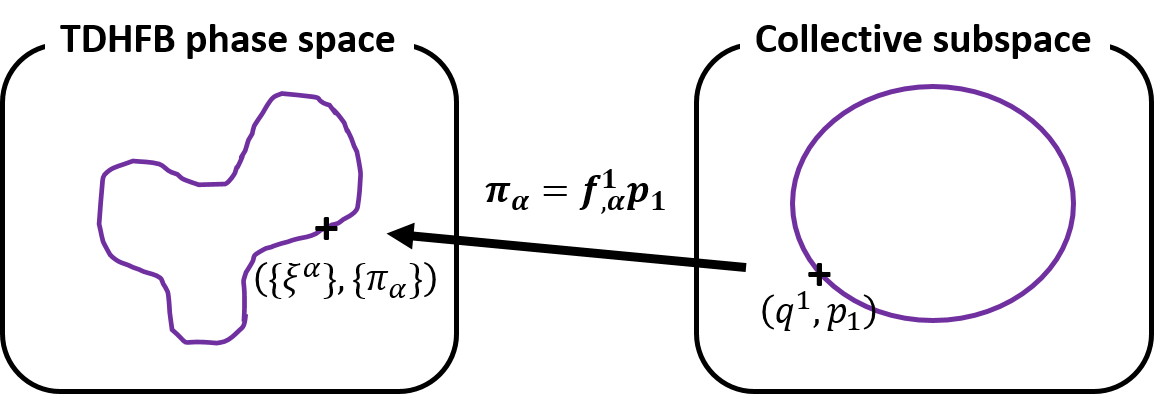
\includegraphics[width=80mm, bb=0 0 550 180]{SPA.png}
% \end{center}
%  \caption{For a TDHFB trajectory, the correspondence between TDHFB phase space and collective subspace.}
%  \label{fig:correspondence}
%\end{figure}
%We try to combine SPA with ASCC. The key point is to find the correspondence between TDHFB phase space and collective subspace in a TDHFB trajectory (See Fig. \ref{fig:correspondence}). We consider the time-dependent state vector $\ket{Z(t)}$ is in a collective subspace. With pairing correlation, $\ket{Z(t)}$ can be expressed as


\subsubsection{(b) Notation and practical procedure for quantization}
\label{sec:notation}

For the application of the ASCC+SPA method to the pairing model in Sec.~\ref{4-2},
we summarize some notations and procedures to obtain quantized states.

In Sec.~\ref{4-2}, the time-dependent generalized Slater determinants
(coherent states) are written as $\ket{Z}$ with complex variables
$Z_\alpha(t)$.
The variables $Z_\alpha$ are transformed into real variables
$(j^\alpha, -\chi_\alpha)$ that correspond to $(\xi^\alpha,\pi_\alpha)$
in Sec.~\ref{4-1}.
The definition and physical meaning of $\chi_\alpha$ and $j^\alpha$ are explained in Sec. \ref{2-2}.
%Although it is customary to take the angle as a coordinate,
%since the angle $\chi_\alpha$ is time-odd quantities, 
%we switch the coordinates and the momenta with minus signs
%in front of variables $\chi$.
Although it is customary to take the time-odd angle $\chi_\alpha$ as a coordinate,
we take the number $j^\alpha$ as a coordinate and the angle $-\chi_\alpha$ as a momentum with an additional minus sign.
Similarly, the gauge angle $\Phi$ and the total particle number $J$
correspond to variables of the pair rotation, $-p_n$ and $q^n$, respectively.
According to the EBK quantization rule (\ref{EBK2}),
the ground state with $k=0$ corresponds to nothing but the HFB state
with a fixed particle number $J(=q^n)$.
For the $k$-th excited states, we perform the following calculations:
\begin{enumerate}
\item Obtain the 1D collective subspace with canonical variables $(q^1,p_1)$
	according to the ASCC in Sec.~\ref{sec:ASCC}.
\item Find a trajectory $(q^1(t),p_1(t))$ which satisfies
the $k$-th EBK quantization condition (\ref{EBK2}).
\item Calculate the action integral (\ref{tau}) for the $k$-th trajectory.
\item Construct the $k$-th excited state using Eq.~(\ref{SPA}).
\end{enumerate}
The ASCC provides the 2D collective subspace $(q^1,J)$
and the generalized coherent states \\
$\ket{\Phi=0,J;q,p=0}$.
For finite values of momenta, we use Eq.~(\ref{momenta2})
to obtain the state $\ket{\Phi,J;q,p}$.

%%%%%%%%%%%%%%%%%%%%%%%%%%%%%%%%%%%%%%%%%%%%

\section{Application of ASCC+SPA in pairing model}
\label{4-2}

\subsection{Application of ASCC}

%In this subsection, we use ($\alpha, \beta, \cdots$) to describe the degrees of freedom instead of $l$ to synchronize the notation with in Sec. \ref{ASCC}. 
We construct a 2D collective subspace $\Sigma_2$ from the ASCC method.
%Because the first order with respect to $\chi_{\alpha}$ is zero in TDHFB Hamiltonian, we assume $j^{\alpha}$ as coordinates and $\chi_{\alpha}$ as conjugate momenta.  The canonical variables are $(j^{\alpha},-\chi_{\alpha})$ and fulfill $\{j^{\alpha},-\chi_{\beta}\}_{PB}=\delta^{\alpha}_{\beta}$. 
We expand the classical Hamiltonian up to second order with respect to
the momenta, $-\chi_{\alpha}$
\begin{align}
  \mathcal{H}(j,\chi) \approx& V(j) + \frac{1}{2}B^{\alpha\beta}(j)\chi_{\alpha}\chi_{\beta},
\end{align}
where the potential $V(j)$ and the reciprocal mass parameter
$B^{\alpha\beta}(j)$ are given as\footnote{In this thesis, $j^{\alpha}$ and $j_{\alpha}$ are identical. Defining the upper index in $j^{\alpha}$ is nothing but to utilize Einstein summation convention.}
%\begin{align}
\begin{eqnarray}
  V(j) &=& \mathcal{H}(j,\chi=0) \nonumber \\
	&=& \sum_{\alpha} 2\epsilon_{\alpha}j^{\alpha} - g\sum_{\alpha} \left[ \Omega_{\alpha}j^{\alpha} - (j^{\alpha})^2 +\frac{(j^{\alpha})^2}{\Omega_{\alpha}} \right] \nonumber \\
  &&- g\sum_{\alpha\ne \beta} \sqrt{j^{\alpha}j^{\beta}(\Omega_{\alpha}-j^{\alpha})(\Omega_{\beta}-j^{\beta})}, \\	
B^{\alpha\beta}(j) &=& \left. \frac{\partial^2\mathcal{H}}{\partial\chi_{\alpha}\partial\chi_{\beta}} \right|_{\chi=0} \\
\label{mass}
&=&
	\begin{cases}
2g\sum_{\gamma\ne \alpha} \sqrt{j^{\gamma}j^{\alpha}(\Omega_{\gamma}-j^{\gamma})(\Omega_{\alpha}-j^{\alpha})}
		& \text{for $\alpha=\beta$} \\
-2g\sqrt{j^{\alpha}j^{\beta}(\Omega_{\alpha}-j^{\alpha})(\Omega_{\beta}-j^{\beta})}
		& \text{for $\alpha\ne\beta$}
	\end{cases}. \nonumber
\end{eqnarray}
%\end{align}
We may apply the ASCC method in Sec. \ref{sec:ASCC}
by regarding $\xi\to j$ and $\pi\to-\chi$.

The TDHFB conserves the average total particle number $N$.
We adopt 
\begin{equation}
	J\equiv N/2=\sum_\alpha j^\alpha, 
  \label{J}
\end{equation}
as a coordinate $q^n$.
Since this is explicitly given as the expectation value of the particle-number
operator, curvature quantities,
such as $f^n_{,\alpha\beta}$ and $f^{(1)n\alpha\beta}$,
are explicitly calculable.
On the other hand, the gauge angle $\Phi=-p_n$ is not given a priori.
Since the ASCC solution provides $g^\alpha_{,n}$ as an eigenvector of
Eq. (\ref{mfQRPA}),
we may construct it as Eq. (\ref{coll_momenta}) in the first order
in $\pi=-\chi$.
We confirm that the pair rotation corresponds to an eigenvector
of Eq. (\ref{mfQRPA}) with the zero frequency $\omega^2=0$.

%With the properties of the constant of motion, we discuss the practical solution of ASCC in pairing model. If we ignore the higher order term $f^{(1)1\alpha\beta}$, we can practice local harmonic equation (LHE)
%\begin{align}
%  B^{\beta\gamma}V_{;\gamma\alpha}f^1_{,\beta}  &= \omega^2 f^1_{,\alpha},\hspace{2em} 
%  B^{\beta\gamma}V_{;\gamma\alpha}g^{\alpha}_{,1} = \omega^2 g^{\beta}_{,1},
%  \label{LHE}
%\end{align}
%which simplifies the moving-frame QRPA equation (\ref{mfQRPA}) by replacing $\tilde{B}^{\beta\gamma}$ into $B^{\beta\gamma}$. Under (\ref{LHE}), 


In the present pairing model, 
from Eq. (\ref{J}), we find $J$ does not depend on $\chi$.
This means $f^{(1)n\alpha\beta}=0$ in Eq. (\ref{q^n}),
thus, $\tilde{B}^{\alpha\beta}=B^{\alpha\beta}$.
The second derivative of $J$ with respect to $j$ also vanishes,
which indicates $f^n_{,\gamma\alpha}$ in Eq.~(\ref{M}) is zero. 
%It indicates the chemical potential $\lambda_I(q)$ is not necessary information to calculate the matrix element in moving-frame QRPA equation.
The gauge angle $\Phi$ is locally determined
by the solution of Eq. (\ref{mfQRPA}).
\begin{align}
%  \Phi = \frac{1}{L}\sum_{\alpha} \chi_{\alpha},
\Phi = g^\alpha_{,n} \chi_{\alpha},
  \label{total_gauge}
\end{align}
%where $L$ is the number of available shells $\alpha=1,\cdots,L$.
%Its conjugate variable
%${\partial\mathcal{L}}/{\partial\dot{\Phi}}$
%is indeed given by $J$ of Eq. (\ref{J}).
%Again, exchanging coordinate and momentum,
%we have $q^n=J$ and $p_n=-\Phi$.

%We consider the treatment for the constant of motion in pairing model. In the TDHFB Hamiltonian, there is no dependence about the total gauge angle
%\begin{align}
%  J \equiv \frac{\partial\mathcal{L}}{\partial\dot{\Phi}}=\sum_{\alpha} j^{\alpha} = \frac{N}{2}
%\end{align}
%is conserved quantity. 

%%%%%% Gauge fixing %%%%%%
It should be noted \cite{N2012} that the definition of the collective
variables $(q^1,p_1)$ is not unique, because it can be arbitrarily mixed
with the pair rotation $(q^n,p_n)$ as
\begin{equation}
	q^1 \rightarrow q^1 + c q^n,  \quad
	p_n \rightarrow p_n -c p_1 \label{eq:pairrotmix}
\end{equation}
with an arbitrary constant $c$.
Numerically, this arbitrariness sometimes leads to a problematic behavior 
in iterative procedure of the ASCC.
In order to fix the parameter $c$, we adopt a condition
called ``ETOP'' in Ref.~\cite{HNMM07}.
We require the following condition to determine $c$:
\begin{align}
\sum_\alpha 
	f^1_{,\alpha} = 0 ,
\end{align}
where $f^1_{,\alpha}$ is replaced as
\begin{align}
{f}^1_{,\alpha} \to f^1_{,\alpha} + c f^n_{,\alpha}
  \label{f}
\end{align}
with Eq. (\ref{eq:pairrotmix}).
%after solving (\ref{LHE}) at each point of $q$.


\subsection{Application of SPA}

After deriving the collective subspace $\Sigma_2$, 
we perform the quantization according to the SPA in Sec.~\ref{sec:SPA}.
Calculating a trajectory in the $(q^1,p_1)$ space,
we can identify a series of states $\{\ket{\Phi,J;q^1(t),p_1(t)}\}$
on the trajectory,
in the form of Eq. (\ref{coherent})
with parameters $Z_\alpha$ given at $(\Phi,J,q^1,p_1)$ and $q^a=p_a=0$ for
$a\geq 3$.
%Due to $J$ is conserved quantity, the action integral can be divided into two terms
Since the variables $(\Phi,J)$ and $(q^1,p_1)$ are separable,
we may take closed trajectories independently in $(\Phi,J)$ and $(q^1,p_1)$
sectors, which we denote here as $C_\Phi$ and $C_1$, respectively.
The action integral is given by
\begin{align}
\mathcal{T}(\Phi,J;q^1,p_1)
=& \int_{C_\Phi} \braket{\Phi(t),J;q^1,p_1|i\frac{\partial}{\partial t}|\Phi(t),J;q^1,p_1} dt \nonumber \\
&+ \int_{C_1} \braket{\Phi,J;q^1(t),p_1(t)|i\frac{\partial}{\partial t}|\Phi,J;q^1(t),p_1(t)} dt
 \nonumber \\
	=& J\Phi + \int_{C_1} \sum_\alpha j^\alpha d\chi_\alpha
	\nonumber \\
	\equiv& \mathcal{T}_\Phi(J,\Phi) +\mathcal{T}_1(q^1,p_1;J) .
%	\label{tau}
\end{align}
In fact, the gauge-angle dependence is formally given as
\begin{equation}
  \ket{\Phi,J;q^1,p_1} = e^{-i\Phi \hat{J}} \ket{J;q^1,p_1},
\end{equation}
where 
\begin{align}
	\hat{J} = \frac{\hat{N}-\nu}{2} = \sum_{\alpha} (\hat{S}_{\alpha}^0 + S_{\alpha}).
\end{align}
Then, the action for the trajectory $C_1$ can be also expressed as
\begin{align}
\mathcal{T}(q^1,p_1;J)=
 \int_{C_1} \braket{J;q^1,p_1|i\frac{\partial}{\partial t}|J;q^1,p_1} dt.
\end{align}
%\begin{align}
%  \mathcal{T}(\Phi,J;q,p) &= \mathcal{T}_{\rm intr}(t) + J\Phi, 
%\end{align}
%%where the intrinsic action integral $\mathcal{T}_{\rm intr}(t)$ becomes
%The important point is $\mathcal{T}_{\rm intr}(t) \ne \int p dq$ at each $t$. For closed TDHFB trajectory, only $\mathcal{T}_{\rm intr}(t)$ contributes to the excited states.

In the SU(2) representation, the invariant measure is
\begin{align}
  d\mu(Z) &= \prod_\alpha \frac{\Omega_\alpha+1}{\pi} (1+|Z_\alpha|^2)^{-2} d({\rm Re}\,Z) d({\rm Im}\,Z) \nonumber \\
&= \prod_\alpha \frac{-(\Omega_\alpha+1)}{4\pi} d(\cos{\theta_\alpha}) d\chi_\alpha \nonumber \\
 &= \prod_\alpha \frac{1+\Omega_\alpha^{-1}}{2\pi} d\chi_\alpha dj^\alpha \nonumber \\
 &= \left[ \prod_\alpha \frac{1+\Omega_\alpha^{-1}}{2\pi} \right] d\Phi dJ dq^1 dp_1 %\nonumber \\
  \prod_a dq^a dp_a,
% d\Phi dJ dq dp = d\Phi dJ dE dt 
	\label{dmu}
\end{align}
where $(q^a,p_a)$ are the intrinsic canonical variables
decoupled from the collective subspace $\Sigma_2$.
In the last line in Eq. (\ref{dmu}),
we used the invariance of the phase-space volume element
in the canonical transformation.
%The part of the invariant measure which contributes to the excited states is
According to Eq. (\ref{dmu}),
the weight function $\rho(q,p)$ in Eq. (\ref{SPA}) is just a constant,
thus, treated as the normalization of the wave function.
%\begin{align}
%d\mu(\Phi,J;q,p) \propto d\Phi dJ dqdp = d\Phi dJ dE dt. 
%\end{align}
%Under EBK quantization condition (\ref{EBK}),

%derive the explicit form of excited states in (\ref{SPA}). From (\ref{GCS}) and (\ref{J}), the state vector $\ket{\Phi,J;q,p}$ becomes
%\begin{align}
%  \ket{\Phi,J;q,p} &= \sum_{\{j_{\alpha}\}} e^{-i\Phi \sum_{\alpha} j_{\alpha}} \ket{J;q,p} .
%\end{align}
The coherent state $\ket{\Phi,J;q^1,p_1}=\ket{Z}$ is
expanded in the SU(2) quasispin basis as
\begin{align}
\ket{Z} &= e^{-i\Phi \hat{J}} \ket{J;q^1,p_1}
 = e^{-i\Phi \hat{J}}\sum_{\{m_\alpha\}} B_m(Z) \ket{\cdots;S_\alpha,-S_\alpha+m_\alpha,\cdots},
\label{coherent2}
\end{align}
where the summation is taken over all possible combinations
of integer values of $\{ m_\alpha\}$ with
\begin{align}
B_m(Z) 
%=& \prod_\alpha 
%\frac{Z_\alpha^{m_\alpha}}
%	{\left(1+|Z_\alpha|^2\right)^{\Omega_\alpha/2}m_\alpha!}
%\sqrt{\frac{\Omega_\alpha! m_\alpha!}{(\Omega_\alpha-m_\alpha)!}} \nonumber\\
% =& \prod_\alpha \left(\frac{1-\cos{\theta}_\alpha}{2}\right)^{m_\alpha/2}\left(\frac{1+\cos{\theta}_\alpha}{2}\right)^{(\Omega_\alpha-m_\alpha)/2}
%\sqrt{\frac{\Omega_\alpha!}{m_\alpha!(\Omega_\alpha-m_\alpha)!}} \\
  =& \prod_\alpha \left(\frac{j_\alpha}{2S_\alpha}\right)^{m_\alpha/2}\left(\frac{2S_\alpha-j_\alpha}{2S_\alpha}\right)^{S_\alpha-m_\alpha/2}
 \sqrt{\frac{(2S_\alpha)!}{m_\alpha!(2S_\alpha-m_\alpha)!}}
e^{-i m_\alpha\phi_\alpha}  ,
	\label{B_m}
\end{align}
where the relative angles are defined as
$\phi_\alpha\equiv\chi_\alpha-\Phi$ and the lower index $m$ indicates a combination of $\{ m_\alpha \}$. From Eq. (\ref{momenta2}) in ASCC, we can directly obtain the relative angles $\phi_\alpha = -f^1_{,\alpha}p_1$.
The integer number $m_\alpha$ corresponds to the number of pairs
in the level $\alpha$.
%is in fixed gauge angle ($\Phi=0$).
%

Using Eq.~(\ref{B_m}),
the $k$-th excited state is calculated as
\begin{align}
\ket{\psi_k} \propto& \oint_{C_\Phi} d\Phi \oint_{C_1} dt
\ket{\Phi,J;q^1,p_1} e^{i\mathcal{T}(\Phi,J;q^1,p_1)}
 \nonumber \\
	=& \sum_{\{m_\alpha\}}
	\int_0^{2\pi} d\Phi e^{i(J-\sum_\alpha m_\alpha)\Phi} \oint dt e^{i\mathcal{T}_1}(t) B_m (Z) \ket{\cdots;S_\alpha,-S_\alpha+m_\alpha,\cdots} \nonumber \\
 \equiv& \sum_{\{m_\alpha\}_J} C_m \ket{\cdots;S_\alpha,-S_\alpha+m_\alpha,\cdots}.
 \label{SPA2}
\end{align}
The coefficients $C_m$ are given by
\begin{align}
C_m = \oint_{C_1} dt e^{i\mathcal{T}_1(t)} B_m(Z(t)).
  \label{coef}
\end{align}
In the last line of Eq. (\ref{SPA2}), the summation is restricted to
$\{m_\alpha\}$ that satisfy $\sum_\alpha m_\alpha=J$.
It is easy to find that $J$ must be integer,
according to the quantization rule (\ref{EBK2}) for the $(J,\Phi)$ sector.

The SPA for the ground state ($k=0$) is given by the stationary point
in the $(q^1,p_1)$ sector,
namely, the HFB state $\ket{\Phi,J;q,p}=e^{-i\Phi\hat{J}}\ket{\rm HFB}$.
Nevertheless, the rotational motion in $\Phi(t)$ is present,
which leads to the number quantization (projection).
Therefore, Eq.~(\ref{SPA2}) becomes
\begin{align}
	\ket{\psi_{\rm g.s.}} \propto& \sum_{\{m_\alpha\}}
	\int_0^{2\pi} d\Phi e^{i(J-\sum_\alpha m_\alpha)\Phi}
	\ket{\rm HFB},  
	\label{SPA3}
\end{align}
which is identical to the wave function of the particle-number projected HFB state.

%%%%%%%%%%%%%%%%%%%%%%%%%%%%%%%%%%%%%%%%%%%

\section{Result}
\label{4-3}
In the pairing model in Chap.~\ref{chap2},
the number of TDHFB degrees of freedom equals that of single-particle levels.
% including the constant of motion (pair rotation). We consider various systems, two-level system, three-level system, and Pb isotope system in each subsection respectively. Next, we discuss the dynamics in non-integrable (more than three-level) system.  
As there are two constants of motion, that is, the particle number and 
the energy, the system is integrable for one- and two-level models.
We first apply the ASCC+SPA method to an integrable two-level model,
then, to non-integrable multi-level models.


\subsection{Integrable case: Two-level pairing model}


\begin{figure}[thb]
 \begin{center}
   \includegraphics[height=0.45\textwidth,angle=-90]{images/N16X3p2trajectory.eps}
 \end{center}
\caption{Classical trajectories satisfying the EBK quantization condition
(\ref{EBK2}) with $k=1$ and 2 in the $(\phi,j)$ phase space.
%The domain of phase space is $-\pi\le\phi<\pi$, $-4\le j\le4$. 
The crosses, solid and dashed lines correspond to the results
of the ASCC+SPA, TDHFB2+SPA, and TDHFB+SPA, respectively.
The crosses for the ASCC+SPA trajectories are plotted every ten calculations
($\delta q = 10dq =0.1/\sqrt{\epsilon_0}$). 
%For the ASCC+SPA trajectories, we plot the crosses
%every ten(?) points of the calculation,
%namely $\delta q=0.1/\sqrt{\epsilon_2-\epsilon_1}$.
}
\label{fig:N16_traj}
\end{figure}
\begin{figure}[thb]
 \begin{center}
   \includegraphics[height=0.5\textwidth,angle=-90]{images/N16X3p2action.eps}
 \end{center}
\caption{Calculated action integrals for the $\ket{0_2^+}$ and $\ket{0_3^+}$ states as functions of time $t$.
The crosses, solid and dashed lines correspond to the ASCC+SPA,
the TDHFB2+SPA, and the TDHFB+SPA, respectively. 
%Dotted lines are the values correspond to EBK quantization condition for $\ket{0_2^+}$ and $\ket{0_3^+}$. 
The action integrals are calculated on each trajectory in Fig. \ref{fig:N16_traj}
from $(\phi,j)=(0,j_{\rm max})$ in the clockwise direction.
The crosses for the ASCC+SPA trajectories are plotted every ten calculations
($\delta q = 10dq =0.1/\sqrt{\epsilon_0}$). 
}
\label{fig:N16_tau}
\end{figure}
\begin{figure}[thb]
 \begin{center}
   \includegraphics[height=0.7\textwidth,angle=-90]{images/N16X3p2occ.eps}
 \end{center}
\caption{
Occupation probabilities for the $0_2^+$ and $0_3^+$ states.
The horizontal line indicates the $j=(m_2-m_1)/2$ of the quasi-spin basis
in Eq. (\ref{SPA2}).
The vertical bars at each $m_2-m_1$ from left to right
represent $|C_m|^2$ of Eq. (\ref{coef}) in
the ASCC+SPA, TDHFB2+SPA and TDHFB+SPA calculations,
respectively.
}
 \label{fig:N16_occ2}
\end{figure}


The two-level pairing model corresponds to the 2D TDHFB system.
Explicitly separating the gauge angle $\Phi$ and
fixing the particle number $J$,
the 2D TDHFB is reduced to the 1D system
with the relative angle $\phi\equiv \chi_2-\chi_1$ and the relative
occupation $j\equiv (j_2-j_1)/2$ as canonical variables.
In Ref.~\cite{NN18}, using the explicit transformation to these
separable variables,
we examined the performance of the SPA requantization
for the two-level model.
In this section, we discuss the same model as in Ref.~\cite{NN18},
but we determine the transformation using the ASCC method and then apply the
SPA (ASCC+SPA).
%In this section, we apply the ASCC+SPA method to the same model.
%In other words, the ASCC method finds the transformation.

Here, we study the system with the equal degeneracy,
$\Omega_1=\Omega_2=8$, 
the pairing strength $g/\epsilon_0=0.2$,
and the particle number $N=16$. 
In this two-level case, we use the level spacing,
$\epsilon_0\equiv \epsilon_2-\epsilon_1$,
as the unit of energy.
The moving-frame QRPA produces the zero mode and another eigenvector
with a finite frequency squared $\omega^2\neq 0$.
We follow the latter mode to construct the collective path.
In the ASCC calculation, we set the increment of the
collective coordinate, $dq=0.01$,
in units of $1/\sqrt{\epsilon_0}$.
We confirm that the pair rotation always has a zero frequency
on the collective path.
On the obtained collective path, we calculate a classical trajectory
for the Hamiltonian
\begin{equation}
\mathcal{H}_{\rm coll}(q^1,p_1;J)=\frac{1}{2} p_1^2 + V(q^1,J)
\end{equation}
with $J=N/2=8$.
Calculated trajectories that satisfy the EBK quantization condition
(\ref{EBK2}) for the first and second excited states ($0_2^+$ and $0_3^+$)
are mapped onto the $(\phi,j)$ plane and
shown in Fig. \ref{fig:N16_traj}.
We also calculate the trajectories using the explicit transformation
of the variables to $(\Phi,J;\phi,j)$, which
are shown by dashed lines in Fig. \ref{fig:N16_traj}.
We call this ``TDHFB trajectories''.
Small deviation in large $\phi$ is due to the absence of the higher-order
terms in $\chi_\alpha$ in the ASCC.
In fact, if we calculate the trajectories in the variables
$(\Phi,J;\phi,j)$ using the Hamiltonian truncated up to the
second order in $\chi_\alpha$ (``TDHFB2 trajectories''),
we obtain the solid lines in Fig. \ref{fig:N16_traj},
which perfectly agree with the ASCC trajectories.

The action integrals $\mathcal{T}(t)$ corresponding to
these closed trajectories are shown in Fig. \ref{fig:N16_tau}.
For the $0_2^+$ state,
all three calculations agree well
with each other, while we see small deviation between the full TDHFB
and the ASCC/TDHFB2 calculations for the $0_3^+$ state.

The calculated wave functions for the excited $0^+$ states 
are shown in Fig. \ref{fig:N16_occ2}. 
We show the occupation probabilities which are decomposed 
into the $2n$-particle-$2n$-hole components. 
The left end of the horizontal axis at $m_2-m_1=-8$ $(j=-4)$
corresponds to a state with $(m_1,m_2)=(N/2,0)$ where all the particles
are in the lower level $\alpha=1$.
The next one at $m_2-m_1=-6$ $(j=-3)$ corresponds to the one with
$(m_1,m_2)=((N-2)/2,1)$, and so on.
The results from the TDHFB2+SPA and the ASCC+SPA are identical to each other
within numerical error, and they reproduce
the TDHFB+SPA calculation well.

%we can obtain the obvious collective path from ASCC.
%The dynamics is exactly identical with adiabatic TDHFB (ATDHFB). We confirm that whether ASCC is identical to one-dimensional ATDHFB, and compare the difference with TDHFB, in numerical calculation.
%
%In two-level system, the classical Hamiltonian in (\ref{TDHFB_Hamiltonian_2}) is
%\begin{align}
%\mathcal{H} 
%  =& \sum_{\alpha=1,2} \epsilon_{\alpha}\Omega_{\alpha}(1- \cos{\theta}_{\alpha})& \nonumber \\ 
% &- \frac{g}{4}\sum_{\alpha=1,2} \Omega_{\alpha} [\Omega_{\alpha}(1-\cos^2{\theta}_{\alpha})+(1-\cos{\theta}_{\alpha})^2] \nonumber \\
%- \frac{g}{2} \Omega_{1}\Omega_{2}&\sqrt{(1-\cos^2{\theta}_{\alpha})(1-\cos^2{\theta}_{\beta})}\cos{(\chi_{2}-\chi_{1})}   .
%\end{align}
%If we define the canonical coordinate $\phi=\chi_2-\chi_1$, it attributes to one-dimensional system. The conjugate momentum is $j= \frac{\partial\mathcal{L}}{\partial\dot{\phi}} = \{\Omega_2(1-\cos{\theta}_2) - \Omega_1(1-\cos{\theta}_1)\}/4$. The ATDHFB indicates that the Hamiltonian can be expanded up to second order with respect to $\phi$
%\begin{align}
%  \mathcal{H}(\phi,j) &\approx V(j) + \frac{1}{2}B^{-1}(j)\phi^2,
%\end{align}
%where $V(j)=\mathcal{H}(\phi=0,j)$ and $B^{-1}(j)= \left. \frac{\partial^2\mathcal{H}}{\partial\phi^2} \right|_{\phi=0}$.
%We know that the BCS ground state corresponds to the potential minimum point with $\phi=0$. If the pairing correlation is strong enough to bind the excited states in the collective potential,  the adiabatic approximation is expected to be well because the states are localized in small $\phi$ region. 
%

By comparing with the full TDHFB calculation with the ASCC+SPA approach
in the two-level pairing model,
we conclude that the ASCC is reliable for description of low-lying
collective states, for which the adiabatic approximation is justifiable.
In addition to that, we should note that the pair rotation is properly separated.
%we succeed to describe the bound collective excited states by ASCC+SPA. For the bound states, whether the adiabatic approximation included or not hardly has influence. Even for the weakly bound states, the adiabatic approximation is reasonable approximation.


\begin{figure*}[tb]
 \begin{center}
  \includegraphics[width=40mm,angle=-90]{images/omega_sq.eps}
 \end{center}
 \caption{Eigenvalues of moving-frame QRPA equation as a function of
the collective coordinate $q^1$, from $N=14$ to $N=24$.
The thick (green) lines are the modes we choose as
the collective coordinate $q^1$,
while the dashed lines correspond to the zero modes ($q^n$).
In each panel, both ends of the horizontal axis corresponds
to the ending points of the collective path $q^1$.
}
 \label{omega_sq}
\end{figure*}
\begin{figure*}[tb]
 \begin{center}
  \includegraphics[width=40mm,angle=-90]{images/occ_number.eps}
 \end{center}
\caption{The occupation numbers $2j^{\alpha}$ in each single-particle level $\alpha$
as a function of the collective coordinate $q^1$,
from $N=14$ to $N=24$.
The purple, green, and blue lines correspond to
$\alpha=1$, 2, and 3, respectively.
At the left end point of the collective coordinate in each panel,
the configuration corresponds to the ``HF-like'' states.
See text for details.
}
 \label{occ_number}
\end{figure*}
\subsection{Non-integrable case (1): Three-level pairing model}
\label{sec:three-level-model}

In contrast to the two-level model,
the TDHFB for the three-level model is non integrable.
%The simplest non-integrable system is three-level system. We have one trivial motion and two time-dependent degrees of freedom. 
We set the parameters of the system as follows:
$\Omega_1=\Omega_2=\Omega_3=\Omega=8$,
$\epsilon_1=-\epsilon_0$, $\epsilon_2=0$, $\epsilon_3=1.5\epsilon_0$,
and $g=0.2\epsilon_0$.
We use the parameter $\epsilon_0$ as the unit energy.
For the sub-shell closed configuration of $N=2\Omega=16$,
the HFB ground state changes from the normal phase to
the superfluid phase at $g_c=0.058\epsilon_0$.
We calculate a chain of systems with even particle numbers
from $N=14$ to $N=24$. 

We obtain three eigen frequencies for the moving-frame QRPA equation, 
on the collective path (Fig. \ref{omega_sq}). 
First of all, we clearly identify the zero mode with $\omega^2=0$
everywhere along the collective path.
This means that the pair rotation is separated from the other
degrees of freedom in the ASCC.
The frequency could become imaginary ($\omega^2<0$).
Except for the case of sub-shell closure ($N=2\Omega_1=16$),
the frequency rapidly increases near the end points.
The end points are given by points where the search for the next point
on the collective path in Sec.~\ref{sec:ASCC} fails.

We choose the lowest frequency squared mode, except for the zero mode,
as a generator of the collective path ($q^1$).
Figure~\ref{occ_number} shows variation of the occupation probability
of each single-particle state, as functions of the collective
coordinate $q^1$ on the collective path.
The most striking feature is that the collective path terminates
with special configurations which are given by the integer number
of occupation.
This is the reason why the search for the collective path fails
at both the ends.
At the end points,
the occupation of the level 3 ($\epsilon_3$) vanishes, while
those of the levels 1 and 2 become either maximum or minimum.
The left end of each panel in Fig.~\ref{occ_number} corresponds to 
a kind of ``Hartree-Fock'' (HF) state which minimizes
the single-particle-energy sum, $\sum_\alpha 2j_\alpha \epsilon_\alpha$.
The pairing correlation is weakened in both ends of the
collective path.

The collective mass with respect to the coordinate $q^1$ is normalized
to unity.
The collective potential is shown in Fig.~\ref{potential}.
The range of $q^1$ is the largest for the system with $N=16$.
This is because the variation of $j^1$ and $j^2$ is the largest in
this case.


\begin{figure}[htbp]
 \begin{center}
  \includegraphics[width=60mm,angle=-90]{images/potential.eps}
 \end{center}
	\caption{Collective potential $V(q^1)$ obtained from the ASCC.
	We adjust the energy minimum point as $q^1=0$ and $V=0$.
}
 \label{potential}
\end{figure}
\begin{table}[htbp]
\begin{center}
\caption{Calculated excitation energies of the first and the second
excited states in units of $\epsilon_0$.
In the exact calculation, the second excited state in the ASCC+SPA
corresponds to the $0_4^+$ state.
See text for details.}
\label{ex}
\begin{tabular}{c|cccccc}
\toprule
            $N$ & $14$ & $16$ & $18$ & $20$ & $22$ & $24$\\ \hline
ASCC+SPA (1st exc.) & $3.87$ & $3.90$ & $3.97$ & $4.09$ & $4.23$ & $4.33$\\
    Exact & $4.09$ & $4.13$ & $4.20$ & $4.30$ & $4.44$ & $4.60$\\ \hline
ASCC+SPA (2nd exc.)& $7.42$ & $7.42$ & $7.60$ & $7.92$ & $8.26$ & $8.47$\\
Exact & $7.65$ & $7.71$ & $7.88$ & $8.15$ & $8.49$ & $8.74$ \\
\bottomrule
\end{tabular}
\end{center}
\end{table}

\begin{figure}[htbp]
 \begin{minipage}{1\hsize}
 \begin{center}
  \includegraphics[height=0.45\textwidth,angle=-90]{images/intra_trans.eps}
  \includegraphics[height=0.45\textwidth,angle=-90]{images/inter_trans.eps}
 \end{center}
 \end{minipage}
\caption{Calculated strength of pair-addition transition (\ref{BPad})
from $N=14$ to $N=22$. 
The solid (dashed) lines correspond to the ASCC+SPA (exact) calculation.
The horizontal line indicates the particle number of the initial states.
The left panel shows the intraband transitions,
$0_1^+\to 0_1^+$ and $0_2^+\to 0_2^+$,
while the right panel shows the interband transitions,
$0_1^+ \to 0_2^+$ and $0_2^+\to 0_1^+$.
}
 \label{3levelPad}
\end{figure}

Based on the collective path determined by the ASCC calculation,
we perform the requantization according to the SPA.
Table \ref{ex} shows the excitation energies of the first and second
excited states, determined by the EBK quantization condition (\ref{EBK2}).
Comparing the result of the ASCC+SPA with that of the exact calculation,
we find that the excitation energies are reasonably well reproduced. 
The ASCC+SPA underestimates the excitation energies only by about 5 \%.
%The difference is that the values from ASCC+SPA are 
%about $5\%$ smaller than exact solution. 

It should be noted that the second excited state in the collective path
corresponds to the $0_4^+$ state,
not to the $0_3^+$ state, in the exact calculation. 
We examine the interband $(k\neq k')$ pair-addition transition,
\begin{equation}
B(P_{\rm ad};k\rightarrow k') \equiv 
	\left|\bra{0_{k'}^+;N+2} \hat{S}^+ \ket{0_k^+;N}\right|^2 ,
\label{BPad}
\end{equation}
in the exact solution.
$B(P_{\rm ad};0_2^+\rightarrow 0_3^+)$ 
is $10\sim100$ times smaller than $B(P_{\rm ad};0_1^+\rightarrow 0_3^+)$,
while $B(P_{\rm ad};0_1^+\rightarrow 0_2^+)$ and
$B(P_{\rm ad};0_1^+\rightarrow 0_3^+)$ are in the same order.
The ASCC+SPA produces states in the same family,
namely, those belonging to the same collective subspace (path).
In the phonon-like picture,
we expect similar magnitude of the strengths for
$B(P_{\rm ad};{\rm g.s.}\rightarrow \omega_{\rm phon})$
and
$B(P_{\rm ad};\omega_{\rm phon}\rightarrow 2\omega_{\rm phon})$,
but smaller values of
$B(P_{\rm ad};{\rm g.s.}\rightarrow 2\omega_{\rm phon})$.
Thus, the $0_4^+$ state in the exact calculation
corresponds to the two-phonon state in the ASCC+SPA.
The $0_3^+$ state in the exact calculation may correspond to
a collective path associated with another solution of the moving-frame QRPA
(thin black line in Fig.~\ref{omega_sq}).

%It indicates that $\ket{0_3^+}$ is also one-phonon state which belongs to the other collective path (black line in Fig. \ref{omega_sq}). About two-phonon states, we can easily find the candidates of two-phonon states from excitation energies and $B(P_{\rm ad};0_1^+\rightarrow 0_{ex}^+)$. In the candidates, $\ket{0_4^+}$ is the lowest two-phonon state and $B(P_{\rm ad};0_2^+\rightarrow 0_4^+)$ is much larger than $B(P_{\rm ad};0_3^+\rightarrow 0_4^+)$. Therefore, $\ket{0_4^+}$ is considered to be most appropriate corresponding to the second excited state in ASCC+SPA calculation.

Next, we calculate the wave functions,
according to Eqs.~(\ref{SPA2}) and (\ref{SPA3}).
The ground state corresponds to the number-projected HFB state
(variation before projection).
In contrast, the excited states are given as superposition of
generalized Slater determinants in the collective subspace,
The pair-addition transition strengths
computed using these wave functions of the excited states
are shown in Fig. \ref{3levelPad}.
For the intraband transition ($k=k'$ in Eq. (\ref{BPad})),
the ASCC+SPA method well reproduces the strengths of the exact calculation.
The ground-to-ground transitions, $B(P_{\rm ad};0_1^+\rightarrow 0_1^+)$, 
are perfectly reproduced, while
$B(P_{\rm ad};0_2^+\rightarrow 0_2^+)$ are underestimated 
by about $10\%\sim20\%$.
\begin{figure*}[tb]
 \begin{center}
  \includegraphics[width=55mm,angle=-90]{images/Pbomega_sq.eps}
 \end{center}
	\caption{The same as described in the caption of Fig. \ref{omega_sq} but for Pb isotopes.
}
 \label{Pb_omega_sq}
\end{figure*}

\begin{figure*}[tb]
 \begin{center}
  \includegraphics[width=55mm,angle=-90]{images/Pbocc_number.eps}
 \end{center}
	\caption{The same as described in the caption of Fig. \ref{occ_number} but for Pb isotopes.
}
 \label{Pb_occ_number}
\end{figure*}

It is more difficult to reproduce the absolute magnitude of
interband transitions ($k\neq k'$), 
which are far smaller than the intraband transitions.
Although the increasing (decreasing) trend for
$B(P_{\rm ad};0_2^+\rightarrow 0_1^+)$
($B(P_{\rm ad};0_1^+\rightarrow 0_2^+)$)
as a function of the particle number is properly reproduced,
the absolute magnitude is significantly underestimated in the ASCC+SPA.
This is due to extremely small collectivity in the interband transitions.
Almost all the strengths are absorbed in the intraband transitions.
Even in the exact calculation, the pair addition strength is
about two orders of magnitude smaller than the intraband strength.
Remember that the non-collective limit ($g\rightarrow 0$) of this
value is $B(P_{\rm ad};0_1^+\rightarrow 0_2^+)=\Omega$.
Therefore, the pairing correlation hinders the interband transitions
by about one order of magnitude.
For such tiny quantities, perhaps, 
the reduction to the 1D collective path is not well justified.
%In our previous study on the two-level case, we found that
%the SPA reasonably well reproduces interband transitions \cite{NN18}.
%The present case corresponds to a strong pairing case with
%the strongly hindered interband transitions.


%It is difficult to reproduce the absolute value of exact solution.
%However, because the pairing correlation is enough strong in this case, the strength of intraband transition is dominant compared with interband transition.
%We can find that 
%$B(P_{\rm ad};0_1^+\rightarrow 0_2^+)$ and $B(P_{\rm ad};0_2^+\rightarrow 0_1^+)$ are only about $1\%$ of $B(P_{\rm ad};0_1^+\rightarrow 0_1^+)$ and $B(P_{\rm ad};0_2^+\rightarrow 0_2^+)$. Therefore, the interband transition can be regarded as reasonable. From all above results, we can conclude that ASCC+SPA reproduces exact solution quantitatively. 

We should remark here that there is a difficulty in the present ASCC+SPA
requantization for weak pairing cases.
In such cases, the potential minimum is close to the left end 
($q^1=q_L$) of the collective path, and the potential height
at $q^1=q_L$, $V(q_L) - V(0)$, becomes small.
Then, a classical trajectory with $E>V(q_L)$ hits this boundary ($q^1=q_L$).
In construction of wave functions,
the boundary condition at $q^1=q_L$ significantly influences the result.
In the present study, we choose a strong pairing case to avoid
such a situation.
As in Fig.~\ref{potential}, the potential height at $q^1=q_L$ has
about $10\epsilon_0$ which is larger than the excitation energies
of the second excitation.
Therefore, all the trajectories are ``closed'' in the usual sense.

%We skipped the result about $\ket{0_3^+}$.

\subsection{Non-integrable case (2): Pb isotopes}
\label{sec:Pb_isotopes}


Finally, we apply our method to neutrons' pairing dynamics in 
neutron-deficient Pb isotopes.
The spherical single-particle levels of neutrons
between the magic numbers 82 and 126 are adopted and
their energies are presented in Table \ref{Pb}. 
The coupling constant $g=0.138$ MeV is determined to reproduce
the experimental pairing gap given by the odd-even mass difference,
$\Delta(N)=\frac{(-1)^{N+1}}{2}[B(N+1)-2B(N)+B(N-1)]$ of ${}^{192}$Pb.
The even-even nuclei from ${}^{188}$Pb to ${}^{194}$Pb
are studied.
\begin{table}[tb]
\begin{center}
\caption{Single-particle energies of Pb isotopes used in the calculation
in units of MeV.
These are obtained from the spherical Woods-Saxon potential
with the parameters of Ref.~\cite{BM69}.
}
\begin{tabular}{c|cccccc}
  \toprule 
  orbit& $h_{9/2}$ & $f_{7/2}$ & $i_{13/2}$ & $p_{3/2}$ & $f_{5/2}$ & $p_{1/2}$\\ \hline
  energy(MeV)& $-10.94$ & $-10.69$ & $-8.74$ & $-8.44$ & $-8.16$ & $-7.45$\\
  \bottomrule 
\end{tabular}
\label{Pb}
\end{center}
\end{table}

The TDHFB dynamics is described by six degrees of freedom.
Figure \ref{Pb_omega_sq} shows eigenvalues of the
moving-frame QRPA equation.
Again, we find that there is a zero mode corresponding to
the neutron pair rotation.
Among the five vibrational modes, we choose the lowest one to
construct the collective path in the ASCC.
This lowest mode never crosses with other modes,
though the spacing between the lowest to the next lowest mode
can be very small, especially for ${}^{194}$Pb.
The evolution of the occupation numbers along the collective path
is shown in Fig. \ref{Pb_occ_number}.
Similarly to the three-level model, 
the end points of the collective path indicate exactly
the integer numbers, and
the left end of each panel corresponds to the
``Hartree-Fock''-like state.
On the collective path, the occupation numbers of $i_{13/2}$, $p_{3/2}$, and
$f_{5/2}$ mainly change.
%The last neutrons are in $i_{13/2}$ from ${}^{188}$Pb to ${}^{194}$Pb. 

\begin{figure}[bt]
 \begin{center}
  \includegraphics[width=60mm,angle=-90]{images/Pbpotential.eps}
 \end{center}
	\caption{The same as Fig. \ref{potential} but for Pb isotopes.
}
 \label{Pb_potential}
\end{figure}
The collective potentials for these isotopes are shown
in Fig. \ref{Pb_potential}.
The heights of the potentials at the left end, $V(q_L)-V(0)$,
are $2\sim3.5$ MeV.
For $^{186}$Pb, the height of the potential is not
enough to satisfy the condition, $E<V(q_L)$,
to have a closed trajectory for the first excited state
(See the last paragraph in Sec.~\ref{sec:three-level-model}).
We encounter another kind of problem for $^{196}$Pb,
which will be discussed in Chapter~\ref{??}.
Therefore, in this paper, we calculate the first excited states
in $^{188,190,192,194}$Pb.


We show the calculated excitation energy of the first excited state
in Table~\ref{Pb_ex}.
Experimentally, this pair vibrational excited $0^+$ state is
fragmented into several $0^+$ states due to other correlations,
such as quadrupole correlation, not taken into account in the present model.
%The value is nothing to do with experimental value because pairing model is too simple to describe realistic nuclear interaction. 
We make a comparison with the exact solution of the multi-level
pairing model.
The ASCC+SPA method quantitatively reproduces the excitation energy of
the exact solution.

\begin{table}[bt]
\begin{center}
\caption{The same as described in the caption of Table \ref{ex} but for Pb isotopes. The energies are given in units of MeV.}
\begin{tabular}{c|cccccc}
  \toprule
   & ${}^{186}$Pb & ${}^{188}$Pb & ${}^{190}$Pb & ${}^{192}$Pb & ${}^{194}$Pb & ${}^{196}$Pb\\ \hline
ASCC+SPA & $-$ & $2.31$ & $2.21$ & $2.12$ & $2.04$ & $-$ \\ 
Exact & $2.58$ & $2.44$ & $2.34$ & $2.25$ & $2.20$ & $2.15$ \\
  \bottomrule
\end{tabular}
\label{Pb_ex}
\end{center}
\end{table}
\begin{figure}[htb]
 \begin{minipage}{1\hsize}
 \begin{center}
  \includegraphics[height=0.45\textwidth,angle=-90]{images/Pbintra_trans.eps}
  \includegraphics[height=0.45\textwidth,angle=-90]{images/Pbinter_trans.eps}
 \end{center}
 \end{minipage}
	\caption{The same as described in the caption of Fig. \ref{3levelPad} but for Pb isotopes.
}
 \label{PbPad}
\end{figure}
The pair-addition transition strengths are shown in Fig. \ref{PbPad}.
The feature that is similar to the three-level case is observed:
dominant intraband transition and very weak interband transitions.
The accuracy from the ASCC+SPA method well reproduces
$B(P_{\rm ad};0_1^+\rightarrow 0_1^+)$
and qualitatively reproduces
$B(P_{\rm ad};0_2^+\rightarrow 0_2^+)$ as well.
The deviation for the latter is about $25\%$.
The interband transitions are smaller than the intraband transitions
by more than two orders of magnitude.
This is also similar to the three-level model discussed
in Sec.~\ref{sec:three-level-model}.
For such weak transitions, the ASCC+SPA significantly
underestimates the strengths.
We may say that the ASCC+SPA gives reasonable results for the intraband
transitions in the realistic values of the pairing coupling constant $g$ and
single-particle levels.


%%%%%%%%%%%%%%%%%%%%%%%%%%%%%%%%%%%%%%%%%

\clearpage{\pagestyle{empty}\cleardoublepage}
\chapter{Collective model treatment}
\label{collective}

The collective model has been proposed
and utilized for the nuclear pairing dynamics
\cite{BBPK70,GPBW85, ZPPRS99, P07}.
For those studies, the pairing collective Hamiltonian is constructed
in terms of the pairing gap parameter $\Delta$ (or equivalent quantities) 
and the gauge angle $\Phi$.  
This is analogous to the Bohr collective model,
in which the collective coordinates are assumed to be the
quadrupole deformation parameters, $\alpha_{2\mu}$.
The 5D collective model has been 
extensively applied to analysis on numerous experimental data.
On the contrary, there have been very few applications of
the pairing collective model
in comparison with experimental data.
In this chapter, we examine the validity of
the collective treatment of the pairing.

Because pairing rotation is trivial, we only consider the collective coordinate for pairing vibration. The deformation parameter is defined in $\alpha\equiv \braket{ \hat{S}^- }$. 
To consider pairing vibration only, we fix the gauge angle as $\Phi=0$.
With $\Phi=0$, the energy minimization with a fixed value of real $\alpha$ always
leads to $\chi_{\alpha}=0$.
\begin{align}
\alpha(j) = \left. \braket{Z|\hat{S}^-|Z} \right|_{\chi=0}
	= \sum_{\alpha} \sqrt{j_{\alpha}(\Omega_{\alpha}-\nu_{\alpha}-j_{\alpha})} .
 \label{Delta}
\end{align}
The parameter $\alpha$ is equivalent to the pairing gap $\Delta$,
since the relation, $\Delta=g\alpha$,
guarantees one-to-one correspondence between $\alpha$ and $\Delta$. 

\section{Integrable system}
In Chapter~\ref{integrable}, we treat $(\phi, j)$ as canonical variables to describe pairing vibration.
The collective model treatment is based on the choice,
$j$ as a coordinate and $\phi$ as a momentum, as discussed in Sec. \ref{ATDHFB}.
\begin{align}
\alpha(j) = \braket{Z|\hat{S}^-|Z}
	= \sqrt{j_1(\Omega_1-\nu_1-j_1)} +\sqrt{j_2(\Omega_2-\nu_2-j_2)},
 \label{Delta_BCS}
\end{align}
where $j_1$ and $j_2$ are the function of $j$ as in (\ref{j_l}).

\begin{figure}[tb]
 \begin{center}
(a) \includegraphics[height=0.44\textwidth,angle=-90]{images/N8p_E.eps}
(b) \includegraphics[height=0.44\textwidth,angle=-90]{images/N16p_E.eps}
 \end{center}
 \caption{Potential surfaces as functions of $j$,
 Eq. (\ref{potential_two_level}) for $x=0.5$, $2$, and $3.2$.
 Dashed line is the pairing deformation parameter $\alpha$
 of Eq.~(\ref{Delta_BCS}) as a function of $j$.
 (a) mid-shell ($\Omega=N=8$) and (b) closed-shell ($2\Omega=N=16$).
}
 \label{fig:p_Delta}
\end{figure}


\begin{figure}[tb]
% \begin{minipage}{0.45\hsize}
 \begin{center}
(a) \includegraphics[height=0.4\textwidth,angle=-90]{images/N50Xeq2p4gap_E.eps}
% \end{center}
% \end{minipage}
% \begin{minipage}{0.45\hsize}
% \begin{center}
(b) \includegraphics[height=0.4\textwidth,angle=-90]{images/N16Xeq2p4gap_E.eps}
 \end{center}
%\end{minipage}
\caption{Potential energy surface as functions of $\alpha$ with $x=2.4$;
(a) $\Omega=N=50$,
(b) $2\Omega=N=16$.
Horizontal lines 
indicate energy spectra. Black lines are obtained
from the potential energy surface, and green lines are 
obtained with the CQ method
(Sec.~\ref{sec:canonical}).
%Left panels: $\Omega=50$, $N=50$ system;
% Right panels: $\Omega=8$, $N=16$ system.
}
 \label{fig:Delta_E}
\end{figure}

The problem is that
there is no one-to-one correspondence between $j$ and $\alpha$.
If we examine the derivative of (\ref{Delta_BCS})
\begin{align}
\frac{\partial\alpha}{\partial j} = \frac{-(\Omega_1-\nu_1)/2+j_1}{\sqrt{j_1(\Omega_1-\nu_1-j_1)}} + \frac{(\Omega_2-\nu_2)/2-j_2}{\sqrt{j_2(\Omega_2-\nu_2-j_2)}} ,
 \label{dalpha}
\end{align}
we can find (\ref{dalpha}) is $+\infty$ for $j_{min}$ and $-\infty$ for $j_{max}$ in any two-level system. It indicates $\frac{\partial\alpha}{\partial j} =0$ exists at $j=j_0$ ($j_{min}<j_0<j_{max}$). For equal degeneracy case ($\Omega_1-\nu_1=\Omega_2-\nu_2$), $j_0=0$. 
The relation between $j$ and $\alpha$ 
are shown by dashed lines in Fig.~\ref{fig:p_Delta} 
for $\Omega=8$ mid-shell (a) and closed-shell (b) configurations discussed in Sec. \ref{SmallOmg}.
The deformation parameter $\alpha$ is largest at $j=0$ (equal filling in both levels),
and smallest at the end points of $j$.
The constrained minimization with respect to $\alpha$ cannot 
produce the states corresponding to $j>0$.
Apparently, we cannot map the entire region of $j$ to $\alpha$.

The collective model treatment
requires the collective wave functions to be well localized
in the $j<0$ region.
The potential energy, $V(j)=\mathcal{H}(\phi=0,j;J=N/2)$ of
Eq. (\ref{potential_two_level}), is also shown in
Fig.~\ref{fig:p_Delta}.
The restriction becomes more serious for the stronger pairing cases.
For instance, the potential with $x=3.2$ in Fig.~\ref{fig:p_Delta}(a)
has only about 1 MeV depth at the minimum point, relative to the value
at the boundary point ($j=0$) corresponding to
the maximum value of $\alpha$ ($\Delta$).

To simulate the result of the collective model, we requantize the ATDHFB Hamiltonian in (\ref{ATDHFB_Hamiltonian})-(\ref{mass_two_level}) by $\hat{\phi}=i\partial/\partial j$, with
the ordering given by Pauli's prescription
\begin{align}
	H \left( j,i\frac{\partial}{\partial j} \right) 
= V(j) - \frac{1}{2}\frac{1}{\sqrt{B(j)}}\frac{\partial}{\partial j}\frac{1}{\sqrt{B(j)}}\frac{\partial}{\partial j}.
\end{align}
The range of the coordinate $j$ is restricted to $j_{\rm min}\leq j \leq 0$
with the vanishing boundary condition $\psi(j_{\rm min})=\psi(0)=0$.
Figure~\ref{fig:Delta_E} shows two examples of the relationship 
between excitation energies and the potential energy surface.
In the panel (a), we show the case of large $\Omega$
($\Omega=50$, $N=50$, and $x=2.4$),
in which
the excited $0^+$ states are bound up to second excitation.
From the collective model, the energies of the ground and the first excited states
are well described, while the deviation becomes larger for
higher excited states.
For very large degeneracy, the pocket of energy surface is deep, 
hence the low-lying excited states may be described by $\alpha$. 
However, in the small-$\Omega$ case ($\Omega=8$, $N=16$, and $x=2.4$)
of the panel (b), no excited states are bound by the potential
as a function of $\alpha$.
None of the excited $0^+$ states
are properly described in the collective model.
This shallow potential is a consequence of the improper
choice of the collective coordinate $\alpha$
which represents only the $j<0$ region.
Therefore, the collective model treatment assuming
$\alpha$ ($\Delta$) as the collective coordinate
is not applicable to small-$\Omega$ and strong-pairing cases.


\section{Non-integrable system}
In Chapter~\ref{non-integrable}, the collective canonical variables $(q^1, p_1)$ describing pairing vibration are obtained from ASCC.
As far as there is a one-to-one correspondence between $\Delta$ 
and the collective variable $q^1$,
we can transform the collective Hamiltonian in $(q^1,\Phi)$
into the one in $(\Delta,\Phi)$. As integrable system, however, we cannot map the entire region of $q^1$ to $\Delta$ because the peak values of pairing gap parameter always appear around the middle of the collective path.

%The pairing gap $\Delta$ is defined as
%\begin{align}
 % \Delta (q) &\equiv \left. g\braket{\Phi,J;q,p|\hat{S}^-|\Phi,J;q,p} \right|_{\Phi=p=0} \nonumber \\
%  &= g\sum_\alpha \sqrt{j^\alpha(\Omega_\alpha-j^\alpha)} .
%\end{align}

In Fig. \ref{q_Delta}, we show two examples of the behavior of pairing gap parameter as a function of the collective coordinate $q^1$.
Panel (a) corresponds to the case of $N=20$ in three-level system ($\Omega_1=\Omega_2=\Omega_3=8$,
$\epsilon_1=-\epsilon_0$, $\epsilon_2=0$, $\epsilon_3=1.5\epsilon_0$,
and $g=0.2\epsilon_0$), and panel (b) corresponds to the case of ${}^{192}$Pb ($g=0.138$ MeV and single-particle level shown in Table \ref{Pb}).
In both panels, the peak in $\Delta$ is near $q^1=0$ and it is not a monotonic
function of $q^1$, thus no one-to-one correspondence exists. 
Because the peak in $\Delta$ emerges near the energy minimum point, the potential surface of $\Delta$ is too shallow to bound first excited states. 
The same behavior observed for all of the non-integrable systems.
The situations are similar to the case in Fig. \ref{fig:Delta_E} (b), where the low-lying excited states cannot be properly described.

We conclude that the pairing gap parameter $\Delta$ (or equivalent quantities) is not a suitable collective coordinate to describe the pairing dynamics, in the multi-level pairing model. 

%Because only one orbit near the Fermi energy ($i_{13/2}$ orbit for both end points) contributes the value of pairing gap, the value at both end points are small compared with the value around the ground state. There is no one-to-one correspondence between $\Delta$ and $q$ not only in ${}^{192}$Pb, but also in all multi-level systems. 


%As with the 5D collective model, pairing can also be supposed as a sort of deformation. The collective model is described by
%the pair deformation parameters pairing gap $\Delta$ and global gauge angle $\Phi$. 
%The utilization of the collective model for nuclear pairing dynamics was done in several references\cite{??}. In our previous study, however, we find that the pairing gap $\Delta$ is not proper to be the collective coordinate in two-level pairing model \cite{??}. In multi-level system, we can investigate the relations between the pairing gap and the collective coordinate. 

\begin{figure}[tb]
 \begin{center}
(a) \includegraphics[height=0.44\textwidth,angle=-90]{images/N20gap.eps}
(b) \includegraphics[height=0.44\textwidth,angle=-90]{images/192Pbgap.eps}
 \end{center}
 \caption{Solid line is the potential surface as a function of $q^1$, and
 dashed line is the pairing gap parameter $\Delta$
 of Eq.~(\ref{Delta}) as a function of $q^1$.
 (a) $N=20$ in three-level system ($\Omega_1=\Omega_2=\Omega_3=8$,
$\epsilon_1=-\epsilon_0$, $\epsilon_2=0$, $\epsilon_3=1.5\epsilon_0$,
and $g=0.2\epsilon_0$), (b) ${}^{192}$Pb ($g=0.138$ MeV and single-particle level shown in Table \ref{Pb}).
}
 \label{q_Delta}
\end{figure}

\clearpage{\pagestyle{empty}\cleardoublepage}
\chapter{Conclusion and perspective}
\label{conclusion}

In order to construct a theoretical framework to describe large-amplitude collective motion associated with nuclear pairing, we studied the low-lying excited $0^+$ states in multi-level pairing model. Based on the time-dependent Hartree-Fock-Bogoliubov (TDHFB) theory, we constructed the pairing collective excited states in two steps: (1) solve the TDHFB equation to obtain the TDHFB classical trajectories; (2) requantize the TDHFB trajectories to obtain the excited states. In these models, the TDHFB degrees of freedom consist of one constant of motion, pairing rotation described in variables $(\Phi, J)$, and $L-1$ degrees of freedom in the system with $L$ single-particle levels. Therefore, the two-level system corresponds to the integrable system, and the system with more than two levels corresponds to the non-integrable system. 

In the integrable two-level case, it is easy to find the coordinates to describe two types of collective motion, pairing rotation described by $(\Phi, J)$, and pairing vibration by variables $(\phi, j)$. With these canonical variables, we studied three different methods of requantization of TDHFB, the stationary-phase approximation (SPA) to the path integral, the canonical quantization (CQ), and the Fourier decomposition (FD) of the time-dependent observables. 
To test the performance of each requantization method, we applied them to systems with large particle numbers, and to small systems which are comparable with the valence orbits in realistic nuclear systems. 
In the former case, all the quantization methods reasonably reproduced the results of the
exact calculation not only for excitation spectra, but also for two-particle transfer matrix elements.
In the later case, on the other hand, the agreement is
less quantitative for the CQ and FD, especially for the two-particle
transfer matrix elements.
In contrast, the SPA keeps its accuracy for both cases in the entire range of
pairing strengths.
One of the reasons of its success is due to the inclusion of the off-diagonal 
parts of the pair transfer operator,
by the explicit construction of the microscopic wave functions.
The CQ and FD calculate the pair transfer matrix elements using only
the diagonal part (expectation value) of the operator $\hat{S}^\pm$,
based on Eqs. (\ref{Sp_mean_value}) and (\ref{Sm_mean_value}).
This is a good approximation when the collectivity is so large that the
diagonal parts dominate.
However, the pairing collectivity may be too weak to justify this
treatment.
Thus, the SPA is the most accurate tool for description of the pairing collective motions in the large-amplitude regime.

The weak point of SPA is that the SPA is applicable only to the
integrable TDHFB systems. To overcome this problem, we proposed the ASCC+SPA method for non-integrable systems. The concept is that the ASCC can decouple an integrable collective subspace from the original TDHFB phase space, then, the SPA is available for the collective subspace.
In this approach, we use the ASCC method to extract the 2D
collective subspace including the pairing rotation.
In other words, we extract an approximate integrable system 
in the non-integrable system described by $(q^1,p_1;J,\Phi)$.

We applied the ASCC+SPA method to the multi-level pairing model.
We investigated the three-level model and 
the multi-level model simulating Pb isotopes
with a realistic pairing coupling constant $g$ and single-particle levels.
In both cases, the low-lying excited $0^+$ states obtained with
the ASCC+SPA well reproduce the exact solutions
not only of the excitation energies but also of the wave functions.
In the ASCC+SPA, the calculation of any matrix elements is straightforward,
because we have a microscopic wave function for every quantized state.
This overcomes a disadvantage in the conventional canonical requantization
in which we need to construct an effective expression of a given operator
in terms of the collective variables only.

We also investigated the validity of the conventional treatment of the pairing
collective model which assumes that the collective coordinate
describing pairing vibration is the paring gap parameter $\Delta$.
In integrable (two-level) systems, the coordinate $j$ describes the pairing vibration.
We have found that there is no
one-to-one correspondence between $\Delta$ and $j$ in any two-level systems.
In non-integrable systems, the coordinate $q^1$ obtained from ASCC describes the pairing vibration. The behavior of $\Delta(q^1)$ is very similar to $\Delta(j)$ in integrable systems. There is no
one-to-one correspondence between $\Delta$ and $q^1$.
The collective
wave functions are not necessarily bound in the region where
the variable $\Delta$ can represent.
Thus, $\Delta$ is not a suitable coordinate to describe pairing vibration, at least in the pairing model.

This is the first attempt of the application of SPA into non-integrable systems, and we succeeded to describe the pairing dynamics quantitatively in the large-amplitude regime. 
In realistic nuclear systems, the competition between pairing and quadrupole correlations is important. The behavior of the pairing dynamics in such systems may be different from that in the pairing model we discussed in this thesis.

Thus, it is of significant interest to apply the SPA to systems with pairing and quadrupole correlations, such as multi-O(4) model \cite{HNMM07} and P+Q model \cite{HNMM08}. It is also important to extend the ASCC+SPA to the following cases: (1) ``unbound'' trajectories in shallow potential energy surface as discussed in Sec. \ref{4-3}; (2) trajectories in potential energy surface with multi energy minimum pockets, such as shape coexistence.
In the former case, we need to find a proper boundary condition to guarantee the periodicity  of the trajectories. In the later case, the tunneling effect between the different energy minimum pockets is important, while the current version of SPA is based on classical trajectories which cannot take into account tunneling effect. Perhaps, it is possible to overcome the difficulty by extending the EBK quantization condition to multi-trajectories in each energy minimum pocket and imaginary-time trajectories in the classically forbidden region.

Ultimately, we aim at applying the ASCC+SPA to the realistic nuclear system with the density functional formalism. The numerical cost for solving the ASCC basic equations is extremely large in realistic systems. Recently, the ASCC has been applied to the realistic nuclear effective interaction \cite{WN16,WN17} employing an efficient method, finite amplitude method (FAM) \cite{NIY07,HKN13}, in solution of the moving-frame QRPA equation. We expect in the near future, ASCC+SPA will be able to describe the low-lying excited states in nuclei, including the mysterious $0^+$ states.



\clearpage{\pagestyle{empty}\cleardoublepage}
\appendix

\chapter{Detailed derivation of the action in pairing model}
\label{derivation}
To obtain the TDHFB dynamics in pairing model, We need to derive the action $\mathcal{S}$ in explicit form. We give the detailed derivation in this chapter.

\section{Matrix elements of the spin-coherent state}
\label{formula1}
The time-dependent coherent state classified into the spin-coherent state is employed in (\ref{coherent}). We derive the necessary formula for the spin-coherent state in this subsection. \par
First, we consider the single-level case.
With the commutation relation in (\ref{SU2commu}), the SU(2) quasispin operators fulfill the following relations
\begin{align}
  \hat{S}^{\pm}\ket{S,S^0} &= \sqrt{(S\mp S^0)(S\pm S^0+1)} \ket{S,S^0\pm 1}
  \label{S_pm} \\
  \hat{S}^0\ket{S,S^0} &= S^0\ket{S,S^0} .
%  \label{S_0}
\end{align}
Using above relations, the coherent state can be expanded as 
\begin{align}
  \ket{Z} &= (1+|Z|^2)^{-S}e^{Z \hat{S}^+}\ket{S,S^0=-S} \nonumber \\
  &= (1+|Z|^2)^{-S}\sum_{n=0}^{2S}\sqrt{\frac{(2S)!}{n!(2S-n)!}}Z^n\ket{S,-S+n} .
\end{align}
We can find the normalization condition is fulfilled
\begin{align}
  \braket{Z|Z} &= (1+|Z|^2)^{-2S}\sum_{n=0}^{2S}\frac{(2S)!}{n!(2S-n)!}|Z|^{2n} \nonumber \\
  &= (1+|Z|^2)^{-2S}\sum_{n=0}^{2S} {}_{2S}\mathrm{C}_n(|Z|^2)^n \nonumber \\
  &= (1+|Z|^2)^{-2S}\times(1+|Z|^2)^{2S} \nonumber \\
  &= 1 .
\end{align}
The overlap is
\begin{align}
  \braket{\eta|Z} &= \frac{(1+\eta^*Z)^{2S}}{(1+|\eta|^2)^S(1+|Z|^2)^S} .
\end{align}

We also calculate the expectation values of the operators. For $\hat{S}^0$,
\begin{align}
  \hat{S}^0e^{Z \hat{S}^+}\ket{S,S^0=-S} &= \sum_{n=0}^{2S}(-S+n)\sqrt{\frac{(2S)!}{n!(2S-n)!}}Z^n\ket{S,-S+n} ,
\end{align}
hence,
\begin{align}
  \braket{Z|\hat{S}^0|Z} &= (1+|Z|^2)^{-2S}\sum_{n=0}^{2S}(-S+n)\frac{(2S)!}{n!(2S-n)!}|Z|^{2n} \nonumber \\
  &= -S + 2S\left( 1-\frac{1}{1+|Z|^2} \right) \nonumber \\
  &= S\left( 1-\frac{2}{1+|Z|^2} \right) .
  \label{S0}
\end{align}
From the first line to the second line, we used the differentiation for the both sides of
\begin{align}
  (1+|Z|^2)^{2S} &= \sum_{n=0}^{2S} {}_{2S}\mathrm{C}_n(|Z|^2)^n
\end{align}
with respect to $|Z|^2$. With (\ref{S0}), the expectation values of occupation number is
\begin{align}
  \braket{Z|\hat{n}|Z} &= \braket{Z|2\hat{S}^0+\Omega|Z} \nonumber \\
	&= 2S\left( 1-\frac{2}{1+|Z|^2} \right) + \Omega .
\end{align}
The expectation values for $\hat{S}^+$ and $\hat{S}^-$ are the complex conjugate pair. For $\hat{S}^+$,
\begin{align}
  \hat{S}^+e^{Z \hat{S}^+}\ket{S,S^0=-S} &= \sum_{n=0}^{2S}\sqrt{(2S-n)(n+1)}\sqrt{\frac{(2S)!}{n!(2S-n)!}}Z^n\ket{S,-S+n+1}.
\end{align}
hence, 
\begin{align}
  \braket{Z|\hat{S}^+|Z} &= (1+|Z|^2)^{-2S}\sum_{n=0}^{2S}Z^n\sqrt{(2S-n)(n+1)}\sqrt{\frac{(2S)!}{n!(2S-n)!}}
  \times(Z^*)^{n+1}\sqrt{\frac{(2S)!}{(n+1)!(2S-n-1)!}} \nonumber \\
    &= (1+|Z|^2)^{-2S} Z^*\sum_{n=0}^{2S}|Z|^{2n}\frac{(2S)!}{n!(2S-n-1)!} \nonumber \\
    &= \frac{2SZ^*}{1+|Z|^2} ,
   \label{S+}
\end{align} 
and
\begin{align}
  \braket{Z|\hat{S}^-|Z} &= \braket{Z|\hat{S}^+|Z}^* = \frac{2SZ}{1+|Z|^2} .
  \label{S-}
\end{align}
For the expectation value of $\hat{S}^+\hat{S}^-$,
\begin{align}
  \braket{Z|\hat{S}^+\hat{S}^-|Z} &= (1+|Z|^2)^{-2S}\|\hat{S}^-e^{Z \hat{S}^+}\ket{S,S^0=-S}\|^2 \nonumber \\
  &= (1+|Z|^2)^{-2S}\sum_{n=0}^{2S}n(2S-n+1){}_{2S}\mathrm{C}_n|Z|^{2n} \nonumber \\
  &= (1+|Z|^2)^{-2S} \left\{ (2S+1)2S(1+|Z|^2)^{2S-1}|Z|^2 - 2S(1+|Z|^2)^{2S}
  \left( \frac{(2S-1)|Z|^4}{(1+|Z|^2)^2}+\frac{|Z|^2}{1+|Z|^2} \right) \right\} \nonumber \\
  &= 2S|Z|^2\frac{2S+|Z|^2}{(1+|Z|^2)^2} .
  \label{S+S-}
\end{align}
From the second line to the third line, we need to calculate the term $\sum_{n=0}^{2S}n^2{}_{2S}\mathrm{C}_n|Z|^{2n}$. It can be obtained from the following relation
\begin{align}
  |Z|^2\frac{\partial}{\partial |Z|^2}|Z|^2\frac{\partial}{\partial |Z|^2}
  (1+|Z|^2)^{2S} &= \sum_{n=0}^{2S}n^2{}_{2S}\mathrm{C}_n|Z|^{2n} .
\end{align}
When $Z$ is time-dependent, the expectation value of $\frac{\partial}{\partial t}$ is also important quantity.
\begin{align}
   \braket{Z|\frac{\partial}{\partial t}|Z} &= \braket{Z|\dot{Z}\frac{\partial}{\partial Z}+\dot{Z}^*\frac{\partial}{\partial Z^*}|Z} \nonumber \\
   &= -\frac{S}{1+|Z|^2}(Z^*\dot{Z}+Z\dot{Z^*}) + \dot{Z}\braket{Z|\hat{S}^+|Z} \nonumber \\
   &= \frac{S}{1+|Z|^2}(Z^*\dot{Z}-Z\dot{Z^*})
\end{align}
From the second line to the third line, we used (\ref{S+}).

Next, we consider the multi-level case. For one-body operators, the extension from the single-level case is simple because we only sum over the index $l$ for the single-particle levels. For two-body operators, we need to give the new derivations basically. For the expectation value of $\hat{S}^+\hat{S}^-$,
\begin{align}
  \braket{Z|\hat{S}^+\hat{S}^-|Z} &= \sum_{\alpha\beta}\braket{Z|\hat{S}_{\beta}^+\hat{S}_{\alpha}^-|Z} .
\end{align}
When $\beta=\alpha$, the form is the same as in (\ref{S+S-}). When $\beta\ne \alpha$, from (\ref{S+}) and (\ref{S-}),
\begin{align}
  \braket{Z|S_{\beta}^+S_{\alpha}^-|Z} = \frac{2S_{\alpha}Z_{\alpha}}{1+|Z_{\alpha}|^2}\frac{2S_{\beta}Z_{\beta}^*}{1+|Z_{\beta}|^2} .
\end{align}
Therefore,
\begin{align}
    \braket{Z|\hat{S}^+\hat{S}^-|Z} = \sum_{\alpha} 2S_{\alpha}|Z_{\alpha}|^2\frac{2S_{\alpha}+|Z_{\alpha}|^2}{(1+|Z_{\alpha}|^2)^2}
    + \sum_{\alpha \neq \beta} \frac{2S_{\alpha}Z_{\alpha}}{1+|Z_{\alpha}|^2}\frac{2S_{\beta}Z_{\beta}^*}{1+|Z_{\beta}|^2} .
\end{align}

We conclude the useful formulae for the spin-coherent state as follows.
\begin{framed}
  \begin{itemize}
 \item Spin-coherent state 
\begin{equation}
	\ket{Z} = \prod_{\alpha} \left(1+|Z_{\alpha}|^2\right)^{-S_{\alpha}}
	e^{Z_{\alpha} \hat{S}_{\alpha}^{+}} \ket{S_{\alpha}, S_{\alpha}^0=-S_{\alpha}} .%
% \label{coherent}
\end{equation}
 \item Normalization
\begin{equation}
	\braket{Z|Z} = 1
\end{equation}
 \item Overlap
\begin{equation}
	  \braket{\eta|Z} = \prod_{\alpha} \frac{(1+\eta_{\alpha}^*Z_{\alpha})^{2S_{\alpha}}}{(1+|\eta_{\alpha}|^2)^{S_{\alpha}}(1+|Z_{\alpha}|^2)^{S_{\alpha}}} .
  \label{overlap}
\end{equation}
 \item Expectation value of $\hat{S}^0$
\begin{equation}
     \braket{Z|\hat{S}^0|Z} = \sum_{\alpha} S_{\alpha}\left( 1-\frac{2}{1+|Z_{\alpha}|^2} \right)
\end{equation}
 \item Expectation value of $\hat{S}^+$
\begin{equation}
     \braket{Z|\hat{S}^+|Z} = \sum_{\alpha} \frac{2S_{\alpha}Z_{\alpha}^*}{1+|Z_{\alpha}|^2}
\end{equation}
 \item Expectation value of $\hat{S}^-$
\begin{equation}
     \braket{Z|\hat{S}^-|Z} = \sum_{\alpha} \frac{2S_{\alpha}Z_{\alpha}}{1+|Z_{\alpha}|^2}
\end{equation}
 \item Expectation value of $\hat{S}^+\hat{S}^-$
\begin{equation}
    \braket{Z|\hat{S}^+\hat{S}^-|Z} = \sum_{\alpha} 2S_{\alpha}|Z_{\alpha}|^2\frac{2S_{\alpha}+|Z_{\alpha}|^2}{(1+|Z_{\alpha}|^2)^2}
    + \sum_{\alpha \neq \beta} \frac{2S_{\alpha}Z_{\alpha}}{1+|Z_{\alpha}|^2}\frac{2S_{\beta}Z_{\beta}^*}{1+|Z_{\beta}|^2}
\end{equation}
 \item Expectation value of $\frac{\partial}{\partial t}$
\begin{equation}
       \braket{Z|\frac{\partial}{\partial t}|Z} = \sum_{\alpha} \frac{S_{\alpha}}{1+|Z_{\alpha}|^2}(Z_{\alpha}^*\dot{Z_{\alpha}}-Z_{\alpha}\dot{Z_{\alpha}^*})
	\label{ddt}
\end{equation}
\end{itemize}
\end{framed}

\section{Matrix elements in special canonical variables $(\chi,j)$ representation}
\label{formula2}
In the text, we mostly use the transformed formulae derived in the previous section.
We use $(\chi,j)$ representation. which is defined from the transformation of the complex number $Z$
\begin{align}
  Z_{\alpha} &\equiv \tan{\frac{\theta_{\alpha}}{2}}e^{-i\chi_{\alpha}} \\
  j_{\alpha} &\equiv S_{\alpha}(1-\cos{\theta}_{\alpha}) .
\end{align}
In such representation, most of matrix elements of spin-coherent state become concise. Because the derivations of the transformation for those matrix elements are simple, we omit the explanation here. We conclude the useful formulae as follows.
\begin{framed}
  \begin{itemize}
 \item Expectation value of $\hat{S}^0$
\begin{equation}
     \braket{Z|\hat{S}^0|Z} = \sum_{\alpha} (j_{\alpha}-S_{\alpha})
\end{equation}
 \item Expectation value of $\hat{S}^+$
\begin{equation}
     \braket{Z|\hat{S}^+|Z} = \sum_{\alpha} \sqrt{j_{\alpha}(2S_{\alpha}-j_{\alpha})}e^{-i\chi_{\alpha}}
\end{equation}
 \item Expectation value of $\hat{S}^-$
\begin{equation}
     \braket{Z|\hat{S}^-|Z} = \sum_{\alpha} \sqrt{j_{\alpha}(2S_{\alpha}-j_{\alpha})}e^{i\chi_{\alpha}}
\end{equation}
 \item Expectation value of $\hat{S}^+\hat{S}^-$
\begin{equation}
    \braket{Z|\hat{S}^+\hat{S}^-|Z} = \sum_{\alpha} \left( 2S_{\alpha} j_{\alpha} - j_{\alpha}^2 +\frac{j_{\alpha}^2}{2S_{\alpha}} \right) 
+ 2\sum_{\alpha\le \beta} \sqrt{j_{\alpha}j_{\beta}(2S_{\alpha}-j_{\alpha})(2S_{\beta}-j_{\beta})}\cos{(\chi_{\alpha}-\chi_{\beta})}   .
\end{equation}
 \item Expectation value of $\frac{\partial}{\partial t}$
\begin{equation}
       \braket{Z|\frac{\partial}{\partial t}|Z} = \frac{1}{i}\sum_{\alpha} j_{\alpha} \dot{\chi_{\alpha}}
	\label{ddt2}
\end{equation}
\end{itemize}
\end{framed}

\section{Derivation of the path integral in spin-coherent state}
We derive the path integral formulation for SU(2) spin-coherent state.
First, we consider the case of one degree of freedom corresponding single-level system.
Using the coherent state $\ket{Z}$, the time development from $t'$ to $t''$ of the system is described by the propagator
\begin{align}
  K(Z'',t'';Z',t') &= \braket{Z''|\exp \left\{-\frac{i}{\hbar}H(t''-t')\right\}|Z'} \\
  &= \lim_{n \to \infty} \int \prod_{k=1}^{n-1}d\mu(Z_k)\prod_{k=1}^{n}
  \braket{Z_k|\exp \left\{-\frac{i}{\hbar}H\epsilon\right\}|Z_{k-1}} ,
  \label{propagator}
\end{align}
where we set $Z_n=Z''$, $Z_0=Z'$, and $\epsilon=\frac{t''-t'}{n}$.
Because $\epsilon$ is infinitesimal quantity, we can expand (\ref{propagator}) with respect to $\epsilon$ up to first order
\begin{align}
  \braket{Z_k|\exp \left\{-\frac{i}{\hbar}H\epsilon\right\}|Z_{k-1}}
  &\approx \braket{Z_k|1-\frac{i}{\hbar}\epsilon H|Z_{k-1}} \nonumber \\
  &\approx \braket{Z_k|Z_{k-1}}\exp\left\{\frac{i}{\hbar}\epsilon
  \frac{\braket{Z_k|H|Z_{k-1}}}{\braket{Z_k|Z_{k-1}}}\right\} \nonumber \\
  &\approx \braket{Z_k|Z_{k-1}}\exp\left\{\frac{i}{\hbar}\epsilon
  \braket{Z_k|H|Z_{k-1}}\right\} .
\end{align}
In addition, we expand the overlap up to first order
\begin{align}
  \braket{Z_k|Z_{k-1}} &= \exp (\log \kappa(Z_k,Z_k^*;Z_{k-1},Z_{k-1}^*)) \nonumber \\
  &\approx \exp \left\{ \frac{i}{\hbar} \left(\frac{\hbar}{i} \left( 
  \frac{\partial \kappa}{\partial Z_k}\Delta Z_k + \frac{\partial \kappa}{\partial Z_k^*}\Delta Z_k^*
  \right) \right) \right\} ,
\end{align}
where we set $\Delta Z_k = Z_k - Z_{k-1} = \dot{Z_k}\epsilon$.
Using (\ref{overlap}), the differentiations of $\kappa$ become
\begin{align}
  \left. \frac{\partial \kappa}{\partial Z_k} \right|_{Z_k=Z_{k-1}} &= -\frac{SZ_k^*}{1+|Z_k|^2}\\
  \left. \frac{\partial \kappa}{\partial Z_k^*} \right|_{Z_k^*=Z_{k-1}^*} &= \frac{SZ_k}{1+|Z_k|^2}
\end{align}
Therefore, the propagator is written in path integral formulation
\begin{align}
    K(Z'',t'';Z',t') &= \int \mathcal{D}\mu(Z(t))e^{\frac{i}{\hbar}\mathcal{S}} \\
     \mathcal{D}\mu(Z(t)) &= \lim_{n \to \infty} \prod_{k=1}^{n-1}d\mu(Z_k) \\
    \mathcal{S} &= \int dt \left\{ \frac{i\hbar S}{1+|Z|^2}(Z^*\dot{Z}-Z\dot{Z^*})
    -\braket{Z|H|Z} \right\}
\end{align}
Of course, the action $\mathcal{S}$ is identical to the definition
\begin{align}
  \mathcal{S} = \int dt \braket{Z|i\hbar\frac{\partial}{\partial t}-H|Z} .
\end{align}
It can be easily checked by using (\ref{ddt}).

The extension to the multi-level system is straightforward. The action $\mathcal{S}$ becomes
\begin{equation}
  \mathcal{S} = \int \mathcal{L}(t) dt, \quad 
  \mathcal{L}(t) =i\hbar \sum_{\alpha} \frac{S_{\alpha}}{1+|Z_{\alpha}|^2}
  (Z_{\alpha}^*\dot{Z_{\alpha}}-Z_{\alpha}\dot{Z_{\alpha}^*}) - \braket{Z|H|Z}
\end{equation}

\section{Action in pairing model}
We derived the action in the previous sections. Using the formula in Sec. \ref{formula1}, the expectation value of pairing Hamiltonian is
\begin{align}
  \braket{Z|H|Z} =& \sum_{\alpha} \epsilon_{\alpha} \left\{ 2S_{\alpha}\left( 1-\frac{2}{1+|Z_{\alpha}|^2} \right) + \Omega_{\alpha} \right\} \nonumber \\
   &- g\sum_{\alpha} 2S_{\alpha}|Z_{\alpha}|^2\frac{2S_{\alpha}+|Z_{\alpha}|^2}{(1+|Z_{\alpha}|^2)^2}
    + \sum_{\alpha \neq \beta} \frac{2S_{\alpha}Z_{\alpha}}{1+|Z_{\alpha}|^2}\frac{2S_{\beta}Z_{\beta}^*}{1+|Z_{\beta}|^2} .
\end{align}
Using the canonical variables $(\chi,j)$, we can obtain the tractable form of the action based on Sec. \ref{formula2}. 
The Lagrangian in $(\chi,j)$ representation becomes
\begin{align}
	\mathcal{L}(t) =& \sum_{\alpha} j_{\alpha}\dot{\chi_{\alpha}} - \mathcal{H}(\chi,j) ,\\
	\mathcal{H}(\chi,j) \equiv& \braket{Z|H|Z} \nonumber \\
	=& \sum_{\alpha} \epsilon_{\alpha}\nu_{\alpha} + \sum_{\alpha} 2\epsilon_{\alpha}j_{\alpha} - g\sum_{\alpha} \left( (\Omega_{\alpha}-\nu_{\alpha}) j_{\alpha} - j_{\alpha}^2 +\frac{j_{\alpha}^2}{\Omega_{\alpha}-\nu_{\alpha}} \right) \nonumber \\
	&- 2g\sum_{\alpha\le \beta} \sqrt{j_{\alpha}j_{\beta}(\Omega_{\alpha}-\nu_{\alpha}-j_{\alpha})(\Omega_{\beta}-\nu_{\beta}-j_{\beta})}\cos{(\chi_{\alpha}-\chi_{\beta})}   .
\end{align}

\clearpage{\pagestyle{empty}\cleardoublepage}
\chapter{Extra discussion in two-level pairing model}

\section{Phase transition point}
\label{two-level}
We consider the phase transition point between the superfluid state and the normal state. The superfluid ground state corresponds to the local minimum point in potential energy surface. The time-dependent coherent state (\ref{coherent}) attributes to BCS trail wave function in $\chi_{\alpha}=0$. For the sake of simplicity, here, we only consider the even-particle system with $\nu=0$ (without Pauli blocking).

With fixed expectation value of the total particle number $N=2J$, the superfluid ground state correspond to the local minimum point in (\ref{Hamiltonian2})
\begin{align}
	\left. \frac{\partial\mathcal{H}(\phi,j;J)}{\partial j} \right|_{\phi=0}=0 .
	\label{dH}
\end{align}
The explicit form of (\ref{dH}) is
\begin{align}
	\frac{2(\epsilon_2-\epsilon_1)}{g} =
	2(S_2q_2-S_1q_1)-(q_2-q_1) + 2\left(\frac{q_2}{\sqrt{1-q_2^2}}S_1\sqrt{1-q_1^2}
	-\frac{q_1}{\sqrt{1-q_1^2}}S_2\sqrt{1-q_2^2}\right) ,
	\label{BCS_2level}
\end{align}
where 
\begin{equation}
	q_{\alpha}=\cos{\theta_{\alpha}} = \frac{\Omega_{\alpha} - J -2(-1)^l j}{\Omega_{\alpha}} 
	\quad \mbox{ for } \alpha=1,2
	\label{q_l}
\end{equation}
with the range $-1\le q_{\alpha}\le 1$. $q_{\alpha}=1$ corresponds to empty occupation and $q_{\alpha}=-1$ corresponds to full occupation. 

(\ref{BCS_2level}) has solution only for the superfluid state. In open shell, (\ref{BCS_2level}) always have solution. In closed shell, substituting $q_1=-1$ and $q_2=1$ into (\ref{BCS_2level}) leads the phase transition point between normal state and superfluid state. The last term of right side in (\ref{BCS_2level}) becomes
\begin{align*}
	& 2\left(\frac{q_2}{\sqrt{1-q_2^2}}S_1\sqrt{1-q_1^2}
	-\frac{q_1}{\sqrt{1-q_1^2}}S_2\sqrt{1-q_2^2}\right) \\
	=\ \ & 2\left(\frac{S_2-j_2}{\sqrt{j_2(2S_2-j_2)}}\sqrt{j_1(2S_1-j_1)}
	- \frac{S_1-j_1}{\sqrt{j_1(2S_1-j_1)}}\sqrt{j_2(2S_2-j_2)}\right) \\
	=\ \ & 2\left(\frac{S_2-j_2}{\sqrt{2S_2-j_2}}\sqrt{j_1}
	- \frac{S_1-j_1}{\sqrt{j_1}}\sqrt{2S_2-j_2}\right) \\ 
	\xrightarrow[j_2\to0]{j_1\to2S_1}\ \ &  4 \sqrt{S_1S_2} .
\end{align*}
From second line to the third line, we used the fact of closed shell $J=2S_1$. With $\Omega_{\alpha}=2S_{\alpha}$, the phase transition point in closed shell is
\begin{align}
	g_c = \frac{2\Delta\epsilon}{\Omega_1+\Omega_2+2\sqrt{\Omega_1\Omega_2}-2} ,
	\label{g_c}
\end{align}
where $\Delta\epsilon=\epsilon_2-\epsilon_1$. When $\Omega_1=\Omega_2=\Omega$, (\ref{g_c}) becomes
\begin{align}
	g_c = \frac{\Delta\epsilon}{2\Omega-1} ,
	\label{g_2}
\end{align}
In the textbook \cite{}, the dimensionless coupling constant $x$ is defined in
\begin{align}
	x = 2g \frac{\Omega}{\Delta\epsilon} .
	\label{x}
\end{align}
We can find the phase transition occurs at
\begin{align}
	x_c = 2g_c \frac{\Omega}{\Delta\epsilon} = \frac{2\Omega}{2\Omega-1} \approx 1.
	\label{x_c}
\end{align}
The last approximation performs well for $\Omega>>1$. We often use the dimensionless coupling constant $x$ in the text. 

\section{Canonical quantization in Pauli's prescription}
\label{can-trans}

In Sec. \ref{integrable}, we derived the TDHFB Hamiltonian in adiabatic approximation. 
The canonical quantization in Pauli's prescription is available for Eq. (\ref{ATDHFB_Hamiltonian}). Using Pauli's prescription, Eq. (\ref{ATDHFB_Hamiltonian}) becomes
\begin{align}
   H \left( j,i\frac{\partial}{\partial j} \right) = V(j) - \frac{1}{2}\sqrt{B^{-1}(j)}\frac{\partial}{\partial j}\sqrt{B^{-1}(j)}\frac{\partial}{\partial j},
\end{align}
and we can obtain the requantized states by solving the Schr\"{o}dinger equation
\begin{align}
   H \left( j,i\frac{\partial}{\partial j} \right) \psi(j) = E \psi(j).
\end{align}

Because the range of $j$ is limited $(j_{\rm min}\le j \le j_{\rm max})$, we have to care about the boundary condition for the end points $j_{\rm min}$ and $j_{\rm max}$. As shown in Fig. ??, the boundary condition is negligible for the strong pairing correlation. On the other hand, the boundary condition is important for the weak pairing correlation because the potential cannot bind the states at $j_{\rm min}$.

We reconsider the coordinate system for the phase space $(\phi,j)$ (Fig. \ref{coordinate}). It is natural to utilize 
a cylindrical coordinate system because $\phi$ is periodic. In cylindrical coordinate system, the points at $j_{\rm min}$ and $j_{\rm max}$ are singular. Instead of the cylindrical coordinate system, we bring an another coordinate system, geographic coordinate system, which assumes the phase space collapsing at $j_{\rm min}$ and  $j_{\rm max}$, such as north pole and south pole. This assumption is available because the (adiabatic) TDHFB Hamiltonian is independent of $\phi$ at $j_{\rm min}$ and $j_{\rm max}$. 


\begin{figure}[htbp]
 \begin{center}
  \includegraphics[width=100mm]{images/can-trans.eps}
 \end{center}
 \caption{Coordinate systems of the phase space $(\phi,j)$ in two-level pairing model. Left figure: cylindrical coordinate system; right figure: geographic coordinate system.}
 \label{coordinate}
\end{figure}

Under the geographic coordinate system, we try to find a new set of canonical variables to obtain the requantized states in weak pairing correlation. 
In $x\to 0$ limit, the excitation energies are $2n\Delta\epsilon$ with equivalent energy spacing because the excited states are pure $2n$-particle-$2n$-hole 
configurations. 
We aim to obtain harmonic oscillator Hamiltonian by canonical transformation 
from $(\phi,j)$ to $(Q,P)$ at $x=0$. We utilize Type III generating function
\begin{align}
G_3(P,\phi) = \frac{P^2}{2\tan{\phi}} - \phi j_{\rm min} .
\end{align}
The first term is known as the harmonic oscillator generating function, 
and the second term is to determine the original point $(q,p)=(0,0)$ at $j=j_{\rm min}$. 
The new canonical variables can be straightforward derived from
\begin{align}
  Q &= -\frac{\partial G_3}{\partial P} = -\frac{P}{2\tan{\phi}} \\
  j &= -\frac{\partial G_3}{\partial \phi} = \frac{P^2}{2\sin{\phi}} + j_{\rm min},
\end{align}
which lead to
\begin{align}
  Q &= \pm \sqrt{2}\sqrt{j-j_{\rm min}} \cos{\phi} \\
  P &= \mp \sqrt{2}\sqrt{j-j_{\rm min}} \sin{\phi}.
\end{align}
Under the new canonical variables, 
we can avoid the singularity at $j=j_{\rm min}$.
Especially at $x=0$, the original classical Hamiltonian becomes
\begin{align}
  \mathcal{H}(\phi,j;J) &= (\epsilon_1+\epsilon_2)J + 2(\epsilon_2-\epsilon_1)j \nonumber \\
  	&= (\epsilon_1+\epsilon_2)J + 2\Delta\epsilon j_{\rm min}
	+ \Delta\epsilon(Q^2+P^2),
\end{align}
which perfectly reproduce the excitation energies $2n\Delta\epsilon$.

%\clearpage{\pagestyle{empty}\cleardoublepage}
%\chapter{Adiabatic self-consistent collective coordinate method}

%\section{Theoretical framework}
%\section{Matrix elements of local harmonic approximation in pairing model}


\clearpage{\pagestyle{empty}\cleardoublepage}
\chapter{Detailed derivation of semiclassical wave function in SPA}
\section{Derivation of Eq. (\ref{semi_wave_func1})}
\label{wave_func1}

We give a derivation of the semiclassical wave function
of Eq. (\ref{semi_wave_func1}).
The explicit form of coherent state in two-level system is

\begin{align}
  \ket{Z} &= \prod_{\alpha=1}^2(1+|Z_{\alpha}|^2)^{-S_{\alpha}}e^{Z_{\alpha}S_{\alpha}^{+}}\ket{0} \nonumber \\
  &= \prod_{\alpha=1}^2\left(1+\tan^2{\frac{\theta_{\alpha}}{2}}\right)^{-S_{\alpha}} \sum_k \frac{1}{k!} \sum_{m=0}^k
  \binom{k}{m} \left(
  \tan{\frac{\theta_1}{2}}e^{-i\phi_1}S_1^{+} \right)^m \left(
  \tan{\frac{\theta_2}{2}}e^{-i\phi_2}S_2^{+} \right)^{k-m} \ket{0} \nonumber \\
  &= \prod_{\alpha=1}^2\left(1+\tan^2{\frac{\theta_{\alpha}}{2}}\right)^{-S_{\alpha}} \sum_k \frac{1}{k!} \sum_{m=0}^k
  \binom{k}{m} \tan^m{\frac{\theta_1}{2}}\tan^{k-m}{\frac{\theta_2}{2}}e^{-ik\Phi}e^{-i(k/2-m)\phi}
  (S_1^{+})^m(S_2^{+})^{k-m} \ket{0}
  \label{ZZ}
\end{align}
Inserting (\ref{ZZ}) into (\ref{semi_wave_func0}) under fixed $J$ and $E_k$,
it becomes
\begin{align}
	\ket{\psi_k^J} \propto& \oint d\Phi \oint dt
	e^{i\mathcal{T}_{J,E_k}(\Phi, t)}
	\ket{\Phi,t}_{J,E_k} \nonumber \\
  \propto& \sum_k \frac{1}{k!} \sum_{m=0}^k \binom{k}{m} \int_0^{2\pi} d\Phi e^{i(J-k)\Phi} 
  \int_0^T dt e^{i\int \pi(t') \dot{\phi}(t') dt'-i(k/2-m)\phi} \nonumber \\
  &\times \left\{ \prod_{\alpha=1}^2\left(1+\tan^2{\frac{\theta_{\alpha}}{2}}\right)^{-S_{\alpha}} \right\}
\tan^m{\frac{\theta_1}{2}}\tan^{k-m}\frac{\theta_2}{2}(S_1^{+})^m(S_2^{+})^{k-m} \ket{0} \nonumber \\
  \propto& \sum_{m=0}^{J} \binom{J}{m} \int_0^T dt \exp{\left( i\int \pi(t') \dot{\phi}(t') dt'-i(J/2-m)\phi \right)} \nonumber \\
  &\times \left\{ \prod_{\alpha=1}^2\left(1+\tan^2{\frac{\theta_{\alpha}}{2}}\right)^{-S_{\alpha}} \right\} 
\tan^m{\frac{\theta_1}{2}}\tan^{J-m}\frac{\theta_2}{2} (S_1^{+})^m(S_2^{+})^{J-m} \ket{0} . \label{semi_wave_func_b}
\end{align}
We find that the integration over $\Phi$ is nothing but the number projection.
In SU(2) quasi-spin representation, the vacuum state is written as
$\ket{0}=\ket{S_1,-S_1;S_2,-S_2}$, which leads to
\begin{align}
  (S_1^{+})^m(S_2^{+})^{J-m} \ket{0} 
  = \sqrt{\frac{(2S_1)!m!}{(2S_1-m)!}} \sqrt{\frac{(2S_2)!(J-m)!}{[2S_2-(J-m)]!}}
  \ket{S_1,-S_1+m;S_2,-S_2+(J-m)}.
\end{align}
For convenience, we define coefficients
\begin{align}
  A(q,S,m) &\equiv 
  \frac{\tan^m{\frac{\theta}{2}}}{\left(1+\tan^2{\frac{\theta}{2}}\right)^{-S}}
  \sqrt{\frac{(2S)!m!}{(2S-m)!}}  \nonumber \\
  &= \left(\frac{j}{2S}\right)^{m/2}\left(\frac{2S-j}{2S}\right)^{S-m/2}
 \sqrt{\frac{(2S)!m!}{(2S-m)!}}
\label{tan}
\end{align}
where $j=S(1-\cos{\theta})$.
Inserting Eq. (\ref{tan}) into Eq. (\ref{semi_wave_func_b}),
we reach Eq. (\ref{semi_wave_func1}).


\section{Derivation of Eq. (\ref{coherent2})}
\label{wave_func2}

To obtain the semiclassical wave function Eq. (\ref{SPA2}) via ASCC, we give the derivation of Eq. (\ref{coherent2}).
%First, we derive the explicit form of coherent state (\ref{coherent2})
\begin{align}
\ket{Z} &= \prod_{\alpha} (1+|Z_{\alpha}|^2)^{-S_{\alpha}}e^{Z_{\alpha}S_{\alpha}^{\dag}}\ket{0} \nonumber \\
&= \prod_{\alpha} \left(1+\tan^2{\frac{\theta_{\alpha}}{2}}\right)^{-S_{\alpha}} \sum_{m_{\alpha}=0}^{2S_{\alpha}} \frac{1}{m_{\alpha}!}
  \left(
  \tan{\frac{\theta_{\alpha}}{2}}e^{-i\chi_{\alpha}}S_{\alpha}^{\dag} \right)^{m_{\alpha}} \ket{0} \nonumber \\
&= \left[ \prod_{\alpha} \left(1+\tan^2{\frac{\theta_{\alpha}}{2}}\right)^{-S_{\alpha}} \right] 
\sum_{\{m_{\alpha}\}} \prod_{\alpha} \frac{1}{m_{\alpha}!} 
  \left(
  \tan{\frac{\theta_{\alpha}}{2}}e^{-i\chi_{\alpha}}S_{\alpha}^{\dag} \right)^{m_{\alpha}} \ket{0} \nonumber \\
&= \left[ \prod_{\alpha} \left(1+\tan^2{\frac{\theta_{\alpha}}{2}}\right)^{-S_{\alpha}} \right] 
\sum_{\{m_{\alpha}\}} \prod_{\alpha} \left(
  \tan{\frac{\theta_{\alpha}}{2}}e^{-i\chi_{\alpha}} \right)^{m_{\alpha}} \sqrt{\frac{(2S_{\alpha})!}{m_{\alpha}!(2S_{\alpha}-m_{\alpha})!}}
  \ket{\cdots;S_{\alpha},-S_{\alpha}+m_{\alpha},\cdots}, 
\label{ZZZ}
\end{align}
where the summation is taken over all possible combinations
of integer values of $\{ m_\alpha\}$. For convenience, we define coefficients
\begin{align}
B_{m_{\alpha}}(q,p) &= \prod_{\alpha} \left(1+\tan^2{\frac{\theta_{\alpha}}{2}}\right)^{-S_{\alpha}} \left(
  \tan{\frac{\theta_{\alpha}}{2}}e^{-i(\chi_{\alpha}-\Phi)} \right)^{m_{\alpha}} \sqrt{\frac{(2S_{\alpha})!}{m_{\alpha}!(2S_{\alpha}-m_{\alpha})!}} \nonumber \\
 &=\prod_\alpha \left(\frac{j_\alpha}{2S_\alpha}\right)^{m_\alpha/2}\left(\frac{2S_\alpha-j_\alpha}{2S_\alpha}\right)^{S_\alpha-m_\alpha/2}
 \sqrt{\frac{(2S_\alpha)!}{m_\alpha!(2S_\alpha-m_\alpha)!}}
e^{-i m_\alpha\phi_\alpha} ,
\end{align}
where $\phi_\alpha \equiv\chi_{\alpha}-\Phi$ and $j_\alpha=S_\alpha(1-\cos{\theta_\alpha})$. Using the coefficients $B_{m_{\alpha}}(q,p)$, Eq. (\ref{ZZZ}) becomes
\begin{align}
  \ket{Z} &= \sum_{\{m_{\alpha}\}} e^{-i\Phi \sum_\alpha m_{\alpha}} B_{m_{\alpha}}(q,p) \ket{\cdots;S_{\alpha},-S_{\alpha}+m_{\alpha},\cdots}.
\label{ZZZ1}
\end{align}
Also, 
\begin{align}
 \ket{Z} &= e^{-i\Phi \hat{J}} \sum_{\{m_{\alpha}\}} B_{m_{\alpha}}(q,p) \ket{\cdots;S_{\alpha},-S_{\alpha}+m_{\alpha},\cdots} \nonumber \\
 &= e^{-i\Phi \sum_{\alpha} (\hat{S}_{\alpha}^0 + S_{\alpha})} \sum_{\{m_{\alpha}\}} B_{m_{\alpha}}(q,p) \ket{\cdots;S_{\alpha},-S_{\alpha}+m_{\alpha},\cdots} \nonumber \\
  &= \sum_{\{m_{\alpha}\}} e^{-i\Phi \sum_\alpha m_{\alpha}} B_{m_{\alpha}}(q,p) \ket{\cdots;S_{\alpha},-S_{\alpha}+m_{\alpha},\cdots}.
\label{ZZZ2}
\end{align}
Comparing Eq. (\ref{ZZZ1}) with (\ref{ZZZ2}), therefore, we reach Eq. (\ref{coherent2}).


\clearpage{\pagestyle{empty}\cleardoublepage}
\chapter{Exact energy spectra in multi-level pairing model}
\section{Two-level system}
We give the energy spectra with various coupling constant $g$ in $\Omega_1=\Omega_2=8$, $\epsilon_1=-\epsilon_0$, and $\epsilon_2=0\epsilon_0$. We fix the seniority as $\nu=0$. The level spacing is $\Delta\epsilon = \epsilon_2-\epsilon_1 = \epsilon_0$. We use a dimensionless coupling constant $x$ as in Eq. (\ref{x}) instead of $g$. $N=16$ corresponds to the closed shell.

\begin{figure}[htbp]
 \begin{center}
  \includegraphics[width=70mm,angle=-90]{images/spectra_x0.eps}
 \end{center}
 \caption{Energy spectra in $x=0$ (no pairing correlation). Horizontal line is total particle number and Vertical line is total energy in units of $\epsilon_0$. Green, light blue, orange, yellow, and deep blue dots correspond to $\ket{0_1^+}\sim\ket{0_5^+}$, respectively.
	}
 \label{x0}
\end{figure}

\begin{figure}[htbp]
 \begin{center}
  \includegraphics[width=70mm,angle=-90]{images/spectra_x0p5.eps}
 \end{center}
 \caption{The same as described in the caption of Fig. \ref{x0} but for $x=0.5$.
	}
 \label{x0p5}
\end{figure}

\begin{figure}[htbp]
 \begin{center}
  \includegraphics[width=70mm,angle=-90]{images/spectra_x1.eps}
 \end{center}
 \caption{The same as described in the caption of Fig. \ref{x0} but for $x=1$.
	}
 \label{x1}
\end{figure}

\begin{figure}[htbp]
 \begin{center}
  \includegraphics[width=70mm,angle=-90]{images/spectra_x2.eps}
 \end{center}
 \caption{The same as described in the caption of Fig. \ref{x0} but for $x=2$.
	}
 \label{x2}
\end{figure}

\begin{figure}[htbp]
 \begin{center}
  \includegraphics[width=70mm,angle=-90]{images/spectra_x3p2.eps}
 \end{center}
 \caption{The same as described in the caption of Fig. \ref{x0} but for $x=3.2$.
	}
 \label{x3p2}
\end{figure}

\begin{figure}[htbp]
 \begin{center}
  \includegraphics[width=70mm,angle=-90]{images/spectra_x8.eps}
 \end{center}
 \caption{The same as described in the caption of Fig. \ref{x0} but for $x=8$.
	}
 \label{x8}
\end{figure}

\newpage

\section{Three-level system}
We give the energy spectra with various coupling constant $g$ in $\Omega_1=\Omega_2=\Omega_3=8$, $\epsilon_1=-\epsilon_0$, $\epsilon_2=0\epsilon_0$, and $\epsilon_3=1.5\epsilon_0$. We fix the seniority as $\nu=0$. $N=16$ and $N=32$ correspond to the closed shell.

\begin{figure}[htbp]
 \begin{center}
  \includegraphics[width=85mm,angle=-90]{images/spectra_g0.eps}
 \end{center}
 \caption{The same as described in the caption of Fig. \ref{x0} but for $g=0\epsilon_0$.
	}
 \label{g0}
\end{figure}

\begin{figure}[htbp]
 \begin{center}
  \includegraphics[width=90mm,angle=-90]{images/spectra_g0p05.eps}
 \end{center}
 \caption{The same as described in the caption of Fig. \ref{x0} but for $g=0.05\epsilon_0$.
	}
 \label{g0p05}
\end{figure}

\begin{figure}[htbp]
 \begin{center}
  \includegraphics[width=90mm,angle=-90]{images/spectra_g0p1.eps}
 \end{center}
 \caption{The same as described in the caption of Fig. \ref{x0} but for $g=0.1\epsilon_0$.
	}
 \label{g0p1}
\end{figure}

\begin{figure}[htbp]
 \begin{center}
  \includegraphics[width=90mm,angle=-90]{images/spectra_g0p15.eps}
 \end{center}
 \caption{The same as described in the caption of Fig. \ref{x0} but for $g=0.15\epsilon_0$.
	}
 \label{g0p15}
\end{figure}

\begin{figure}[htbp]
 \begin{center}
  \includegraphics[width=90mm,angle=-90]{images/spectra_g0p2.eps}
 \end{center}
 \caption{The same as described in the caption of Fig. \ref{x0} but for $g=0.2\epsilon_0$.
	}
 \label{g0p2}
\end{figure}

\bibliographystyle{unsrt}
\bibliography{ref}


\end{document}
